\documentclass{article}

\usepackage[letterpaper,top=2cm,bottom=2cm,left=2.9cm,right=2.9cm,marginparwidth=1.75cm]{geometry}

\usepackage[english]{babel}
\usepackage{amsmath}
\usepackage{graphicx}
\usepackage{setspace}
\usepackage{import}
\usepackage{float}
\usepackage{xcite}
\usepackage[hidelinks]{hyperref}
%\usepackage{xr}
\usepackage{xcolor}
\usepackage[font=footnotesize, labelfont=bf]{caption}

\setcounter{page}{0}

\usepackage{tocloft}
\setlength{\cftsecnumwidth}{3em}
\setlength{\cftsubsecnumwidth}{3em}
\setlength{\cftsubsubsecnumwidth}{4em}

\begin{document}

\renewcommand{\thepage}{S\arabic{page}} 
\renewcommand{\thesection}{S\arabic{section}}  
\renewcommand{\thetable}{S\arabic{table}}  
\renewcommand{\thefigure}{S\arabic{figure}}

% --------------------------
\thispagestyle{empty}
\begin{center}
~~ \\ 
\bigskip 
\bigskip 
\bigskip 
\bigskip 
\bigskip 
\bigskip 
\bigskip 
\bigskip 
\bigskip 
\bigskip 
\bigskip 
\bigskip 
\bigskip 
\bigskip 
    \Huge Appendices: Global poverty estimation using private and public sector big data sources \\
    \bigskip
    \bigskip
    \bigskip
    \Huge 
\end{center}
    \bigskip
    \bigskip
    \bigskip
    \bigskip
    \bigskip
    \bigskip
    \bigskip
    \bigskip
    \bigskip
    \bigskip
    \bigskip
    \bigskip
    \bigskip
    \bigskip
    \bigskip
    \bigskip
    \bigskip
    \bigskip
    \bigskip
    \bigskip
    \bigskip
    \bigskip
    \bigskip

% --------------------------
\newpage
\tableofcontents

% --------------------------
\newpage
\doublespacing
\section{DHS summary statistics}

\singlespacing
\begin{table}[H]
\small
\caption{DHS summary statistics of countries used for estimating levels of wealth}
\label{tab:dhs_summary_table}
\centering
\begin{tabular}{l ccc} 
\hline 
Country & DHS Year & N        & Global Wealth Index \\ 
        &          & Clusters & Mean (sd) \\ 
\hline 
Albania & 2017 & 715 & 2.59 (0.68)  \\ 
 Angola & 2015 & 625 & -1.2 (1.4)  \\ 
 Armenia & 2015 & 313 & 2.78 (0.54)  \\ 
 Bangladesh & 2017 & 672 & -0.34 (1.03)  \\ 
 Benin & 2017 & 540 & -1.01 (0.92)  \\ 
 Bolivia & 2008 & 997 & 0.56 (1.41)  \\ 
 Burkina Faso & 2017 & 224 & -1.85 (0.88)  \\ 
 Burundi & 2016 & 552 & -2.14 (0.73)  \\ 
 Cambodia & 2014 & 611 & 0.04 (1.17)  \\ 
 Cameroon & 2018 & 430 & -0.57 (1.25)  \\ 
 Chad & 2014 & 624 & -2.77 (0.75)  \\ 
 Colombia & 2010 & 4868 & 1.88 (1.4)  \\ 
 Comoros & 2012 & 242 & -0.05 (0.99)  \\ 
 Congo - Kinshasa & 2013 & 492 & -2.81 (0.9)  \\ 
 Côte d’Ivoire & 2011 & 341 & -0.58 (1.14)  \\ 
 Dominican Republic & 2013 & 524 & 1.52 (0.84)  \\ 
 Egypt & 2014 & 1817 & 2.63 (0.62)  \\ 
 Eswatini & 2006 & 270 & -0.02 (1.46)  \\ 
 Ethiopia & 2019 & 305 & -1.95 (1.25)  \\ 
 Gabon & 2012 & 332 & -0.13 (1.33)  \\ 
 Gambia & 2019 & 280 & 0.23 (1.19)  \\ 
 Ghana & 2019 & 192 & 0.01 (0.78)  \\ 
 Guatemala & 2014 & 853 & 0.99 (1.32)  \\ 
 Guinea & 2018 & 401 & -1.1 (1.37)  \\ 
 Guyana & 2009 & 312 & 0.62 (1.14)  \\ 
 Haiti & 2016 & 450 & -1.39 (1.04)  \\ 
 Honduras & 2011 & 1128 & 0.42 (1.39)  \\ 
 India & 2015 & 28358 & 0.07 (1.25)  \\ 
 Indonesia & 2002 & 1319 & 0.32 (1.28)  \\ 
 Jordan & 2017 & 970 & 2.85 (0.72)  \\ 
 Kenya & 2020 & 298 & -0.86 (1.08)  \\ 
 Kyrgyzstan & 2012 & 314 & 1.29 (0.7)  \\ 
 Lesotho & 2014 & 399 & -1.38 (1.09)  \\ 
 Liberia & 2019 & 321 & -1.84 (0.69)  \\ 
 Madagascar & 2016 & 358 & -2.25 (0.77)  \\ 
 Malawi & 2017 & 148 & -1.54 (1.1)  \\ 
 Mali & 2018 & 328 & -1.03 (1.16)  \\ 
 Moldova & 2005 & 399 & 1.72 (1.12)  \\ 
 Morocco & 2003 & 480 & 1.29 (1.76)  \\ 
 Mozambique & 2018 & 221 & -1.55 (1.37)  \\ 
 Myanmar (Burma) & 2015 & 441 & -0.62 (0.86)  \\ 
 Namibia & 2013 & 550 & 0.15 (2.01)  \\ 
 Nepal & 2016 & 383 & -0.52 (1.01)  \\ 
 Niger & 2012 & 476 & -2.8 (1.12)  \\ 
 Nigeria & 2018 & 1382 & -0.5 (1.13)  \\ 
 Pakistan & 2017 & 560 & 0.77 (1.35)  \\ 
 Peru & 2009 & 1131 & 0.57 (1.57)  \\ 
 Philippines & 2017 & 1213 & 0.61 (0.8)  \\ 
 Rwanda & 2019 & 500 & -1.62 (0.8)  \\ 
 Senegal & 2019 & 214 & -0.27 (1.23)  \\ 
 Sierra Leone & 2019 & 557 & -1.68 (0.98)  \\ 
 South Africa & 2016 & 746 & 1.85 (1.45)  \\ 
 Tajikistan & 2017 & 365 & 1.29 (0.93)  \\ 
 Tanzania & 2017 & 436 & -1.47 (0.99)  \\ 
 Timor-Leste & 2016 & 455 & -0.55 (1.17)  \\ 
 Togo & 2017 & 171 & -0.83 (0.88)  \\ 
 Uganda & 2018 & 316 & -1.9 (0.88)  \\ 
 Zambia & 2018 & 535 & -1.45 (1.44)  \\ 
 Zimbabwe & 2015 & 400 & -0.3 (1.79)  \\ 
 \hline 
\end{tabular}
\end{table}
\normalsize
\doublespacing

\singlespacing
\begin{table}[H]
\small
\caption{DHS summary statistics of countries used for estimating changes in wealth}
\label{tab:dhs_summary_table_changes}
\centering
\begin{tabular}{l | ccc | ccc} 
\hline 
Country & \multicolumn{3}{c}{1st Survey Closest to 2000} & \multicolumn{3}{c}{Latest Survey} \\ 
        & Year & N        & Global Wealth Index      & Year & N        & Global Wealth Index    \\ 
        &      & Clusters & Mean (sd)                &      & Clusters & Mean (sd)      \\ 
\hline 
Albania & 2008 & 450 & 2.47 (0.75)  & 2017 & 715 & 2.67 (0.68)   \\ 
 Angola & 2006 & 115 & -0.86 (1.62)  & 2015 & 625 & -0.81 (1.4)   \\ 
 Armenia & 2010 & 308 & 2.57 (0.67)  & 2015 & 313 & 2.75 (0.54)   \\ 
 Bangladesh & 1999 & 341 & -1.35 (1.29)  & 2017 & 672 & -0.55 (1.03)   \\ 
 Benin & 2001 & 247 & -0.94 (1.17)  & 2017 & 540 & -0.73 (0.92)   \\ 
 Burkina Faso & 1998 & 208 & -1.41 (0.98)  & 2017 & 224 & -1.05 (0.88)   \\ 
 Burundi & 2010 & 376 & -1.87 (0.92)  & 2016 & 552 & -1.92 (0.73)   \\ 
 Cambodia & 2000 & 470 & -1.22 (1.01)  & 2014 & 611 & 0.16 (1.17)   \\ 
 Cameroon & 2004 & 464 & -0.81 (1.28)  & 2018 & 430 & -0.32 (1.25)   \\ 
 Congo - Kinshasa & 2007 & 293 & -1.7 (1.06)  & 2013 & 492 & -1.88 (0.9)   \\ 
 Côte d’Ivoire & 1998 & 140 & 0.42 (1.4)  & 2011 & 341 & -0.36 (1.14)   \\ 
 Dominican Republic & 2007 & 1425 & 1.28 (1.04)  & 2013 & 524 & 1.69 (0.84)   \\ 
 Egypt & 2000 & 998 & 1.67 (1.15)  & 2014 & 1817 & 2.6 (0.62)   \\ 
 Ethiopia & 2000 & 535 & -1.95 (0.86)  & 2019 & 305 & -1.4 (1.25)   \\ 
 Ghana & 1998 & 400 & -0.72 (1.16)  & 2019 & 192 & 0.15 (0.78)   \\ 
 Guinea & 1999 & 293 & -1.31 (1.09)  & 2018 & 401 & -0.7 (1.37)   \\ 
 Haiti & 2000 & 316 & -1.12 (1.22)  & 2016 & 450 & -1.13 (1.04)   \\ 
 Jordan & 2002 & 495 & 3.23 (0.43)  & 2017 & 970 & 2.86 (0.72)   \\ 
 Kenya & 2003 & 399 & -1.25 (1.32)  & 2020 & 298 & -0.66 (1.08)   \\ 
 Lesotho & 2004 & 381 & -1.47 (0.74)  & 2014 & 399 & -1.01 (1.09)   \\ 
 Liberia & 2007 & 291 & -1.81 (0.58)  & 2019 & 321 & -1.59 (0.69)   \\ 
 Madagascar & 2008 & 585 & -1.35 (0.92)  & 2016 & 358 & -1.43 (0.77)   \\ 
 Malawi & 2000 & 560 & -1.92 (0.79)  & 2017 & 148 & -1.31 (1.1)   \\ 
 Mali & 2001 & 399 & -1.47 (1.12)  & 2018 & 328 & -0.54 (1.16)   \\ 
 Mozambique & 2009 & 270 & -1.39 (1.18)  & 2018 & 221 & -1 (1.37)   \\ 
 Namibia & 2000 & 260 & -0.14 (2.13)  & 2013 & 550 & 0.38 (2.01)   \\ 
 Nepal & 2001 & 251 & -1.41 (1.45)  & 2016 & 383 & -0.51 (1.01)   \\ 
 Niger & 1998 & 268 & -1.72 (0.97)  & 2012 & 476 & -1.5 (1.12)   \\ 
 Nigeria & 2003 & 360 & -0.39 (1.38)  & 2018 & 1382 & -0.3 (1.13)   \\ 
 Pakistan & 2006 & 957 & 0.04 (0.2)  & 2017 & 560 & 0.95 (1.35)   \\ 
 Peru & 2000 & 1408 & 0.56 (1.82)  & 2009 & 1131 & 0.94 (1.57)   \\ 
 Philippines & 2003 & 816 & 1.02 (1.35)  & 2017 & 1213 & 0.63 (0.8)   \\ 
 Rwanda & 2005 & 456 & -2.01 (0.62)  & 2019 & 500 & -1.45 (0.8)   \\ 
 Senegal & 2005 & 366 & -0.57 (1.34)  & 2019 & 214 & -0.04 (1.23)   \\ 
 Sierra Leone & 2008 & 350 & -1.59 (0.86)  & 2019 & 557 & -1.38 (0.98)   \\ 
 Tajikistan & 2012 & 343 & 1.24 (1.06)  & 2017 & 365 & 1.52 (0.93)   \\ 
 Tanzania & 1999 & 173 & -1.72 (0.93)  & 2017 & 436 & -1.32 (0.99)   \\ 
 Timor-Leste & 2009 & 454 & -1.24 (1.08)  & 2016 & 455 & -0.36 (1.17)   \\ 
 Togo & 1998 & 287 & -1.13 (0.82)  & 2017 & 171 & -0.63 (0.88)   \\ 
 Uganda & 2000 & 267 & -1.61 (1.03)  & 2018 & 316 & -1.36 (0.88)   \\ 
 Zambia & 2007 & 319 & -1.31 (1.36)  & 2018 & 535 & -1.02 (1.44)   \\ 
 Zimbabwe & 1999 & 221 & -0.47 (1.78)  & 2015 & 400 & -0.06 (1.79)   \\ 
 \hline 
\end{tabular}
\end{table}
\normalsize
\doublespacing

% --------------------------
\newpage
\section{Comparing DHS wealth index and global wealth index}
\label{si:comparing_dhs_global_wi}

\begin{figure}[H]
    \centering
    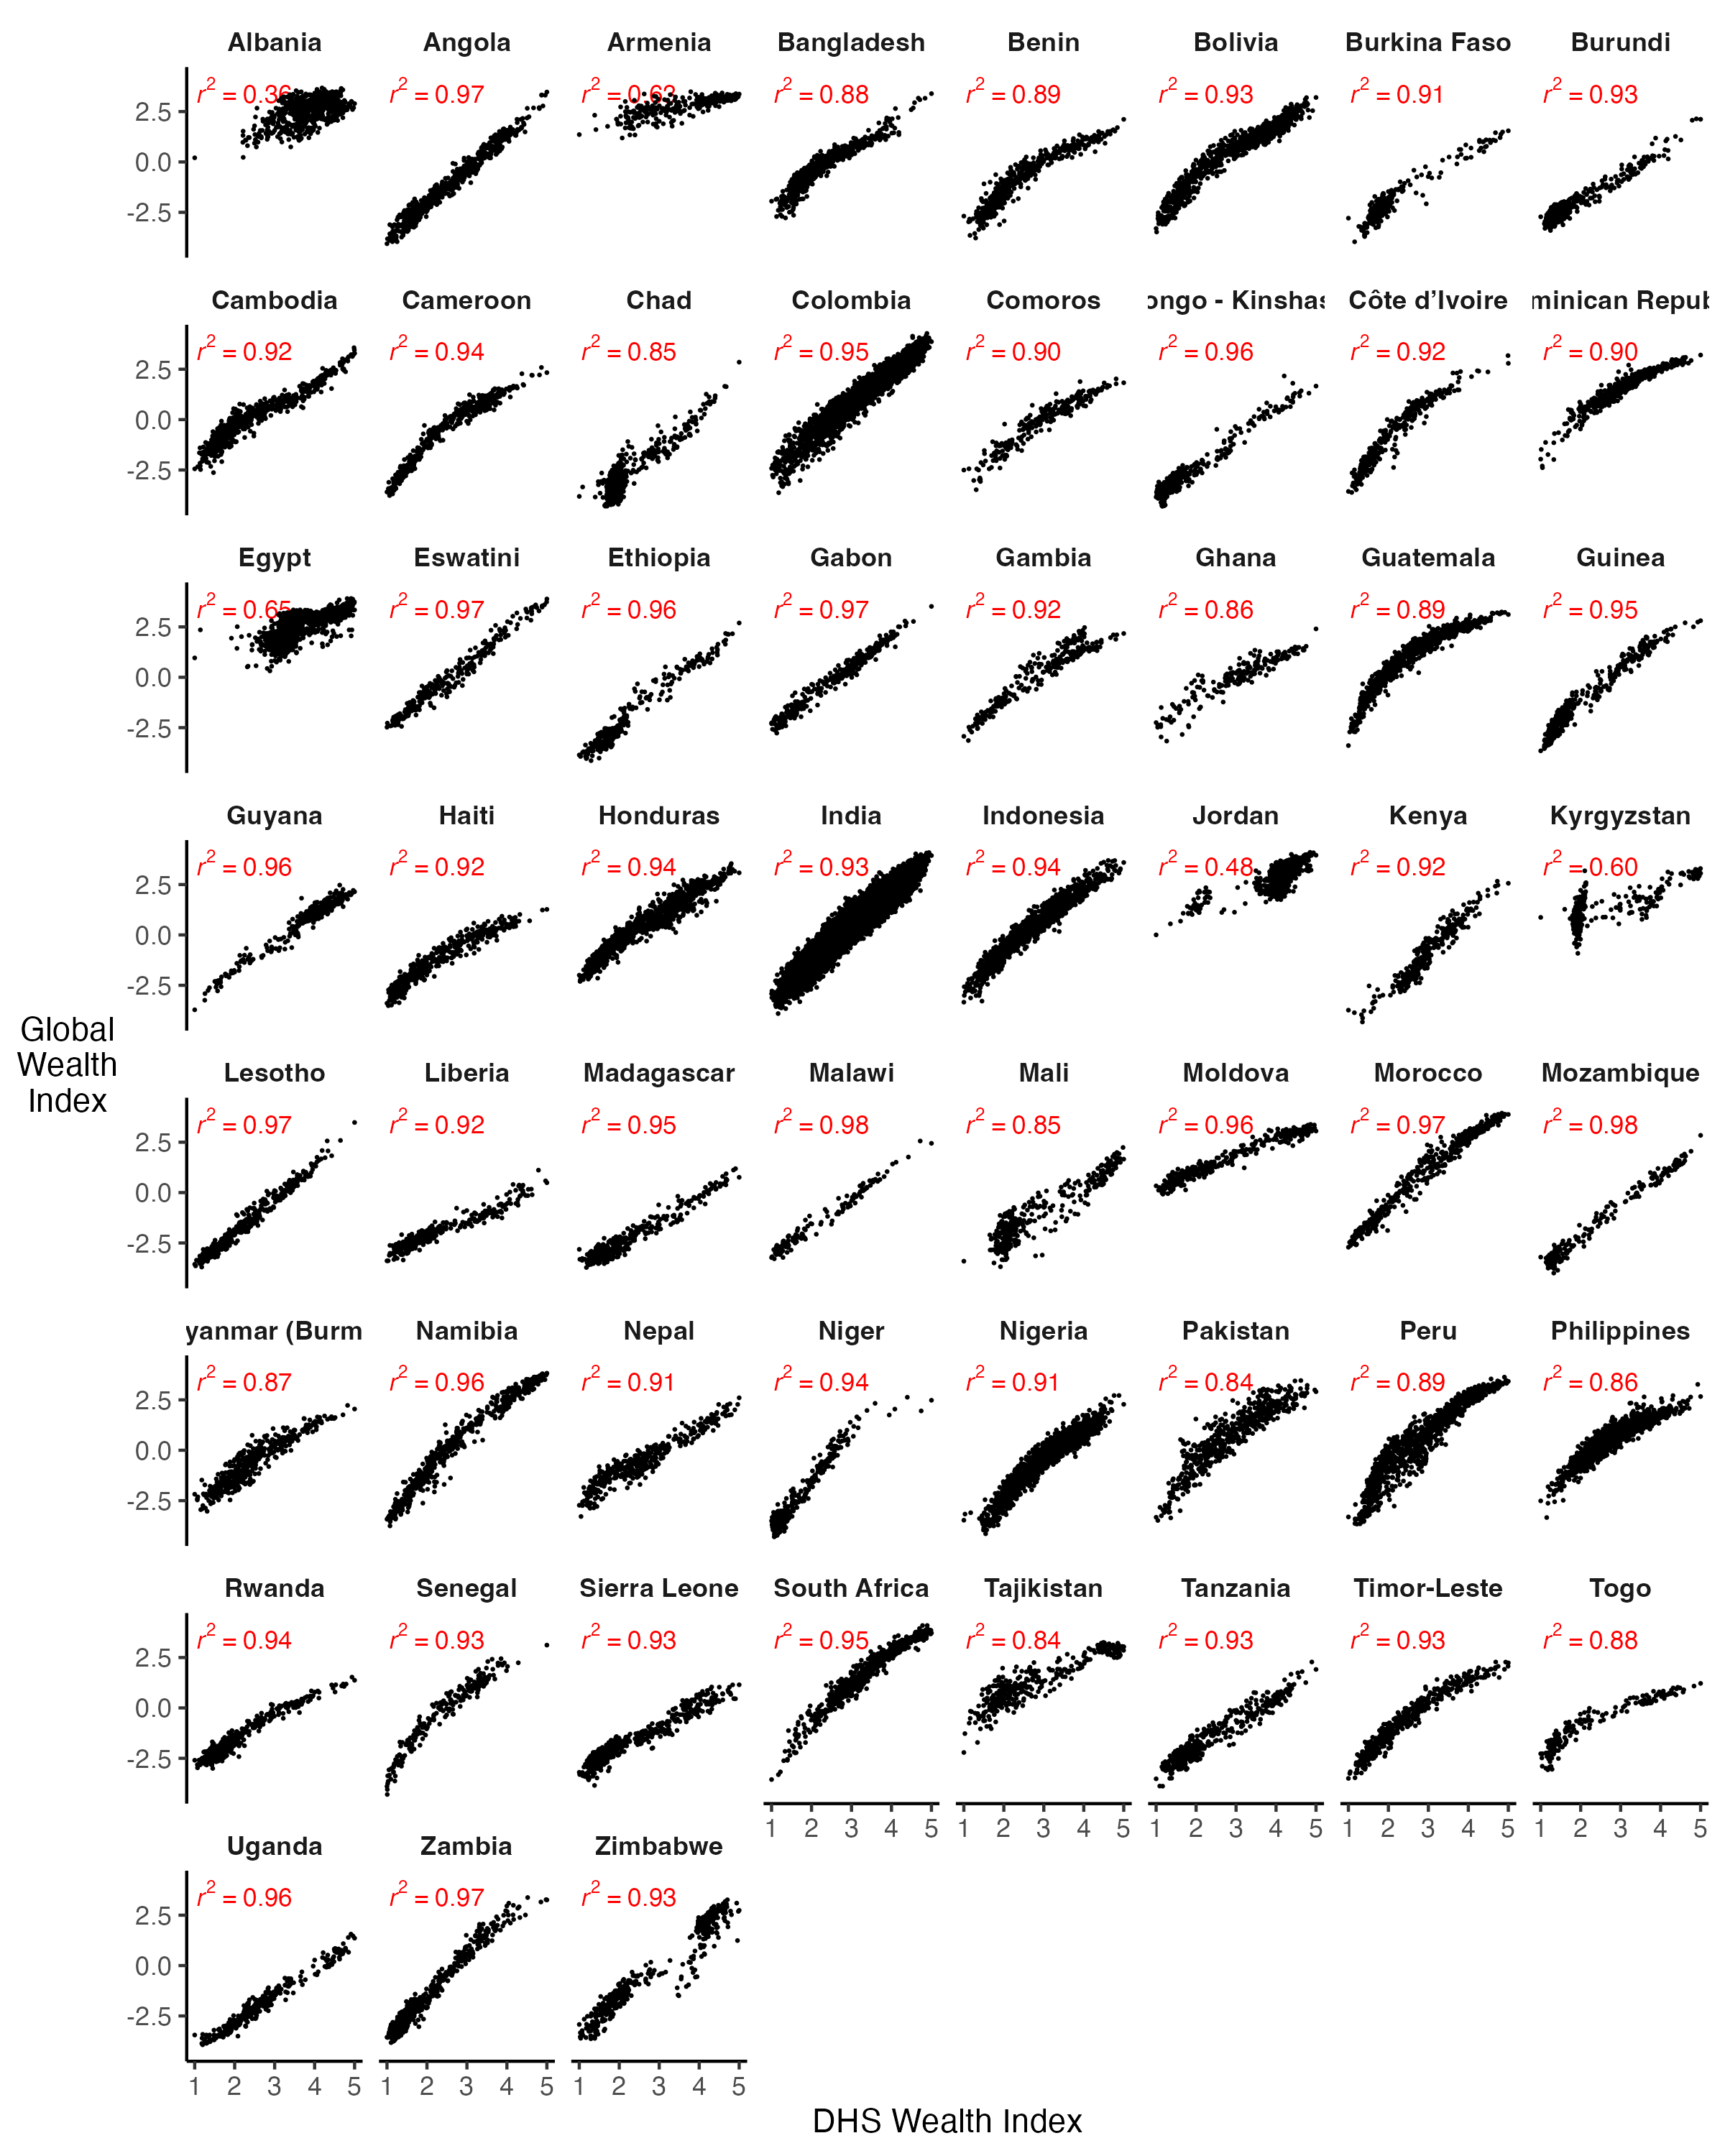
\includegraphics[width=0.8\textwidth]{figures/dhsindex_globalindex_cor.png}
    \caption{Association between DHS wealth index and global wealth index for each country}
     \label{fig:dhsindex_globalindex_cor}
\end{figure}

% --------------------------
\newpage
\section{Correlation of Facebook features with wealth index for each country}
\label{si:cor_fb_wi}

\begin{figure}[H]
    \centering
    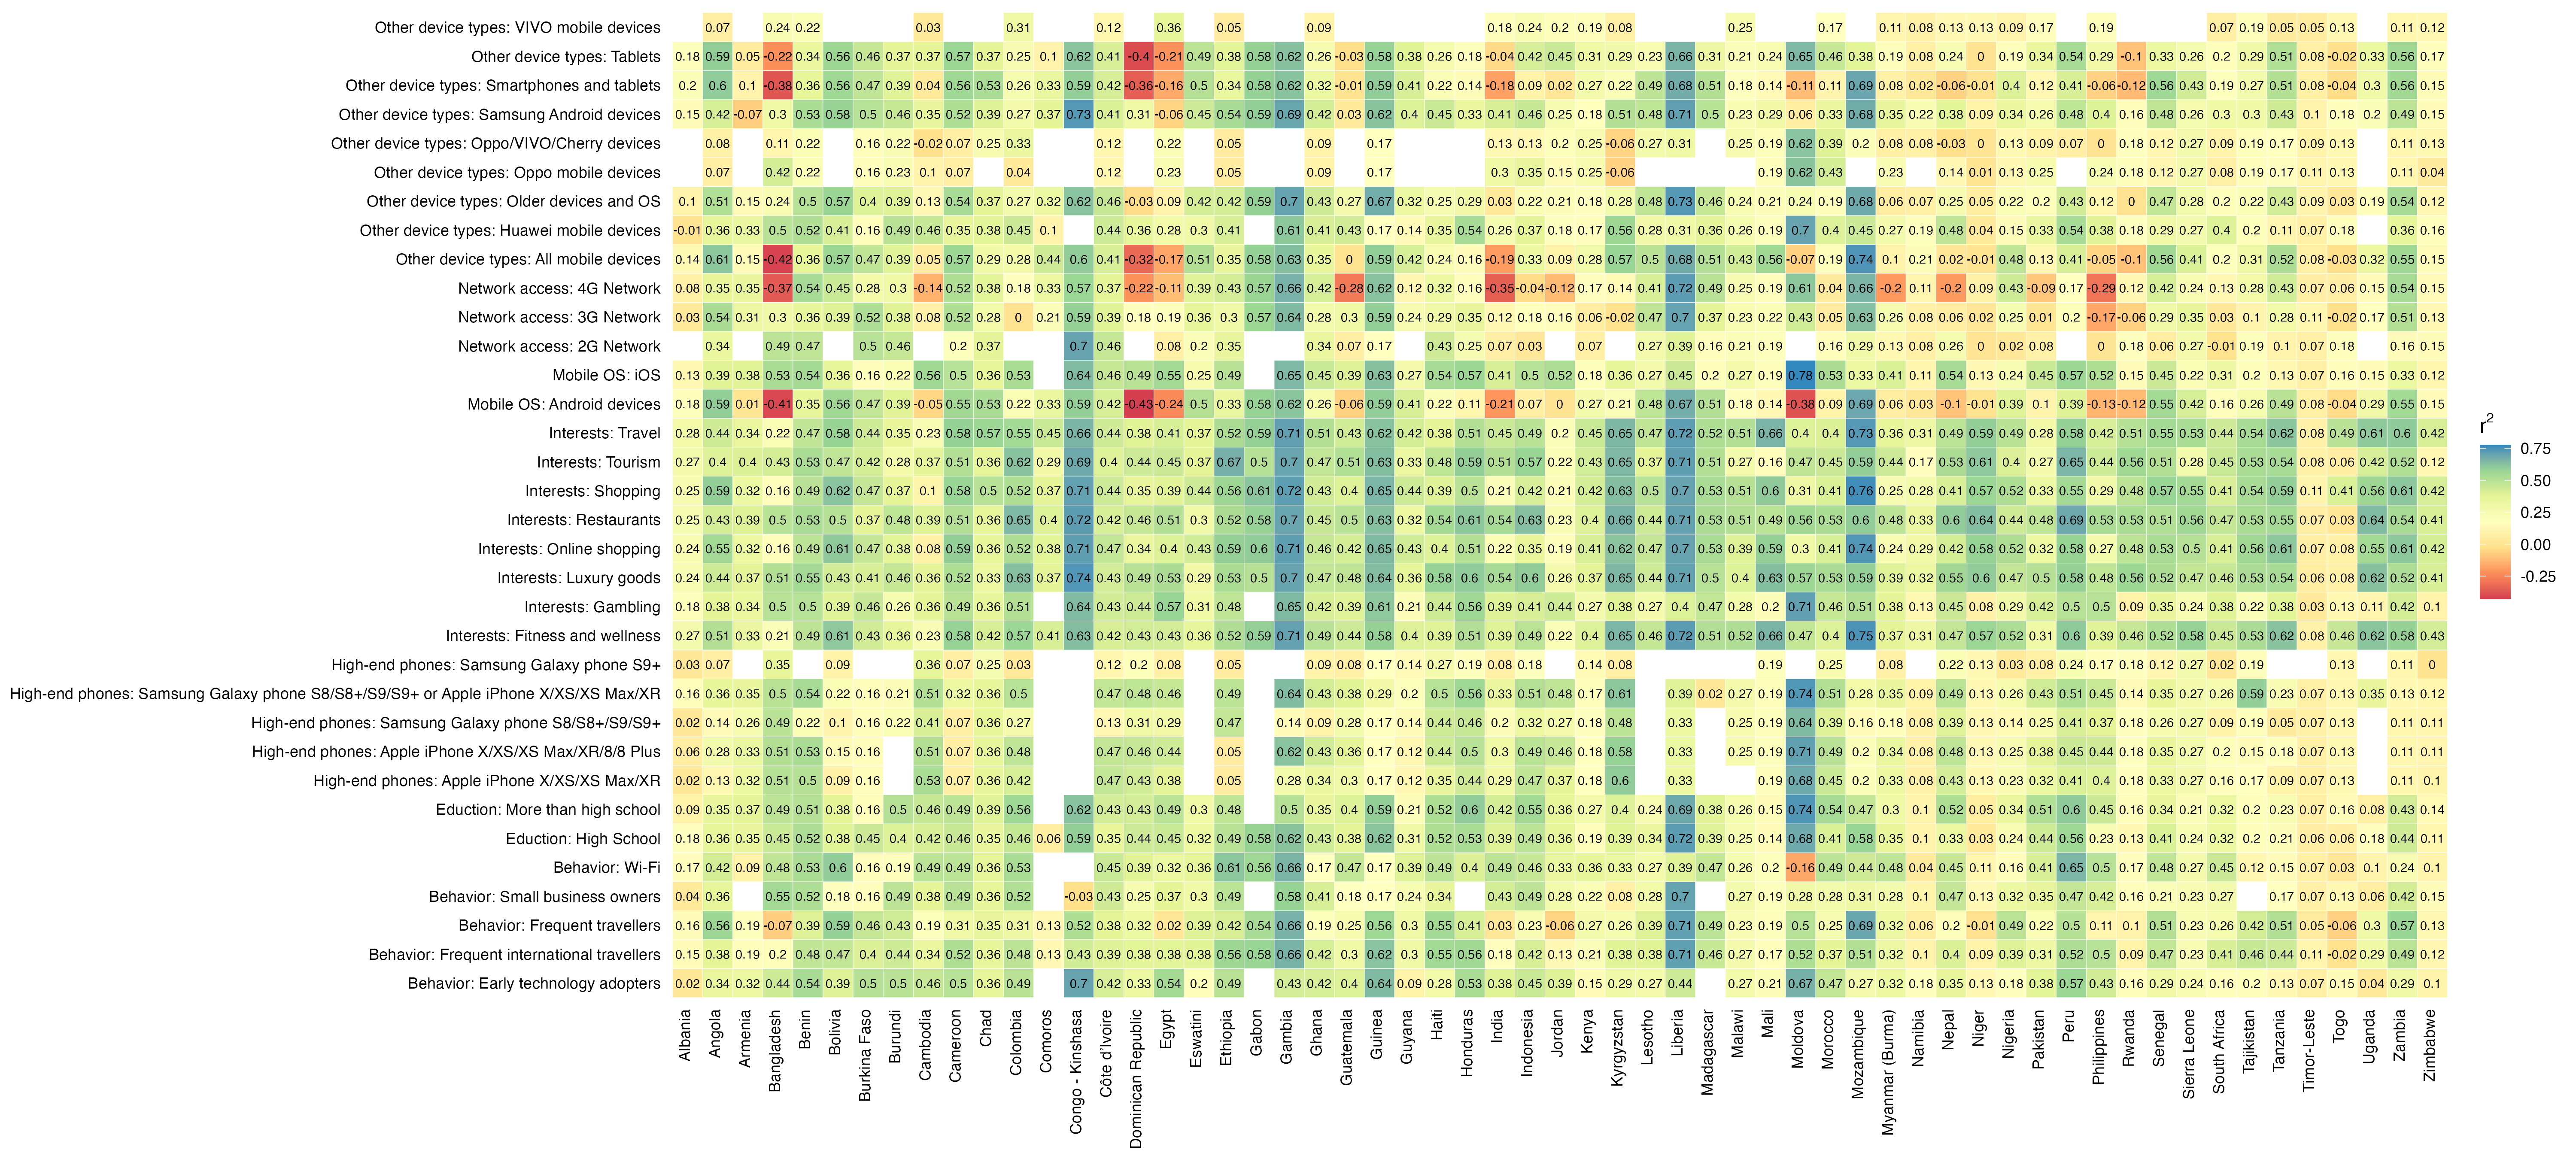
\includegraphics[width=1\textwidth]{figures/fb_features_cor_each_country.png}
    \caption{Correlation of Facebook features with wealth index}
     \label{fig:fb_features_cor_each_country}
\end{figure}

% --------------------------
\newpage
\section{Within country correlation of top features}
\label{si:within_cor_top_features}

\begin{figure}[H]
    \centering
    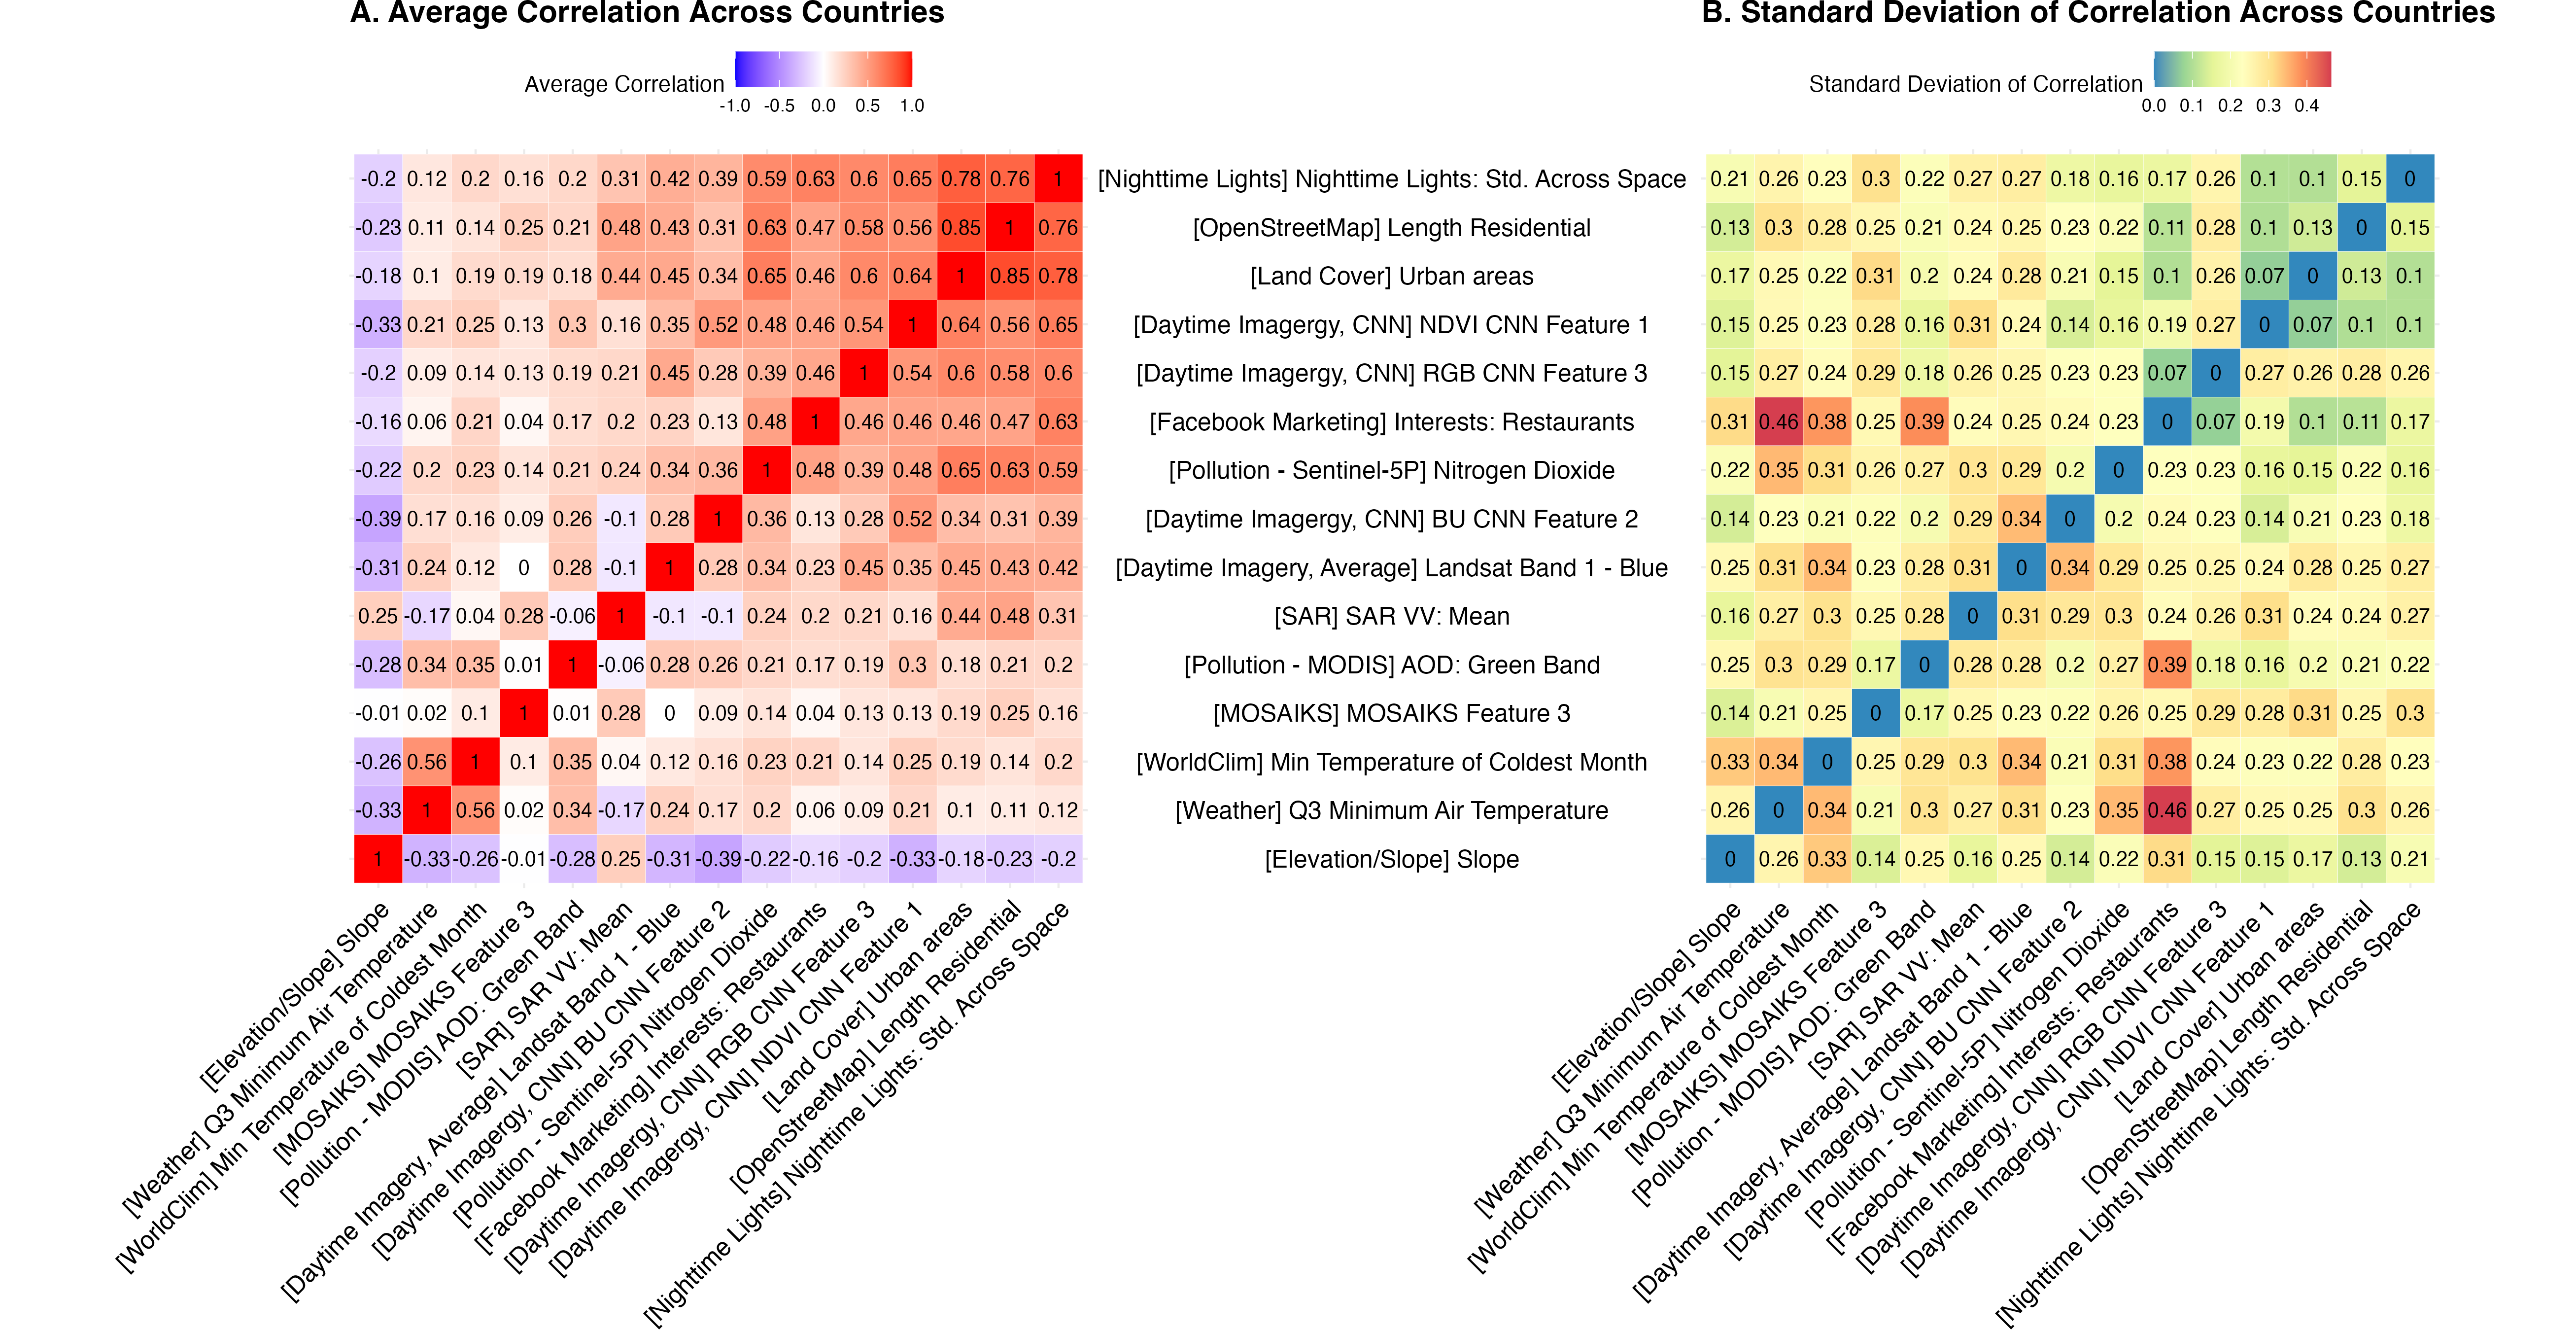
\includegraphics[width=1\textwidth]{figures/cor_between_vars.png}
    \caption{Correlation of variables between each other. We use the variable with the highest correlation to the wealth score in each dataset. {\bf Panel A} shows the average correlation across countries and {\bf panel B} shows the standard deviation in correlations across countries. The variables are ordered top to bottom and right to left according to their correlation with the wealth score.}
     \label{fig:cor_between_vars}
\end{figure}

% --------------------------
\newpage
\section{Scatterplots of true and estimated levels wealth for each country}
\label{si:scatter_levels}

\begin{figure}[H]
    \centering
    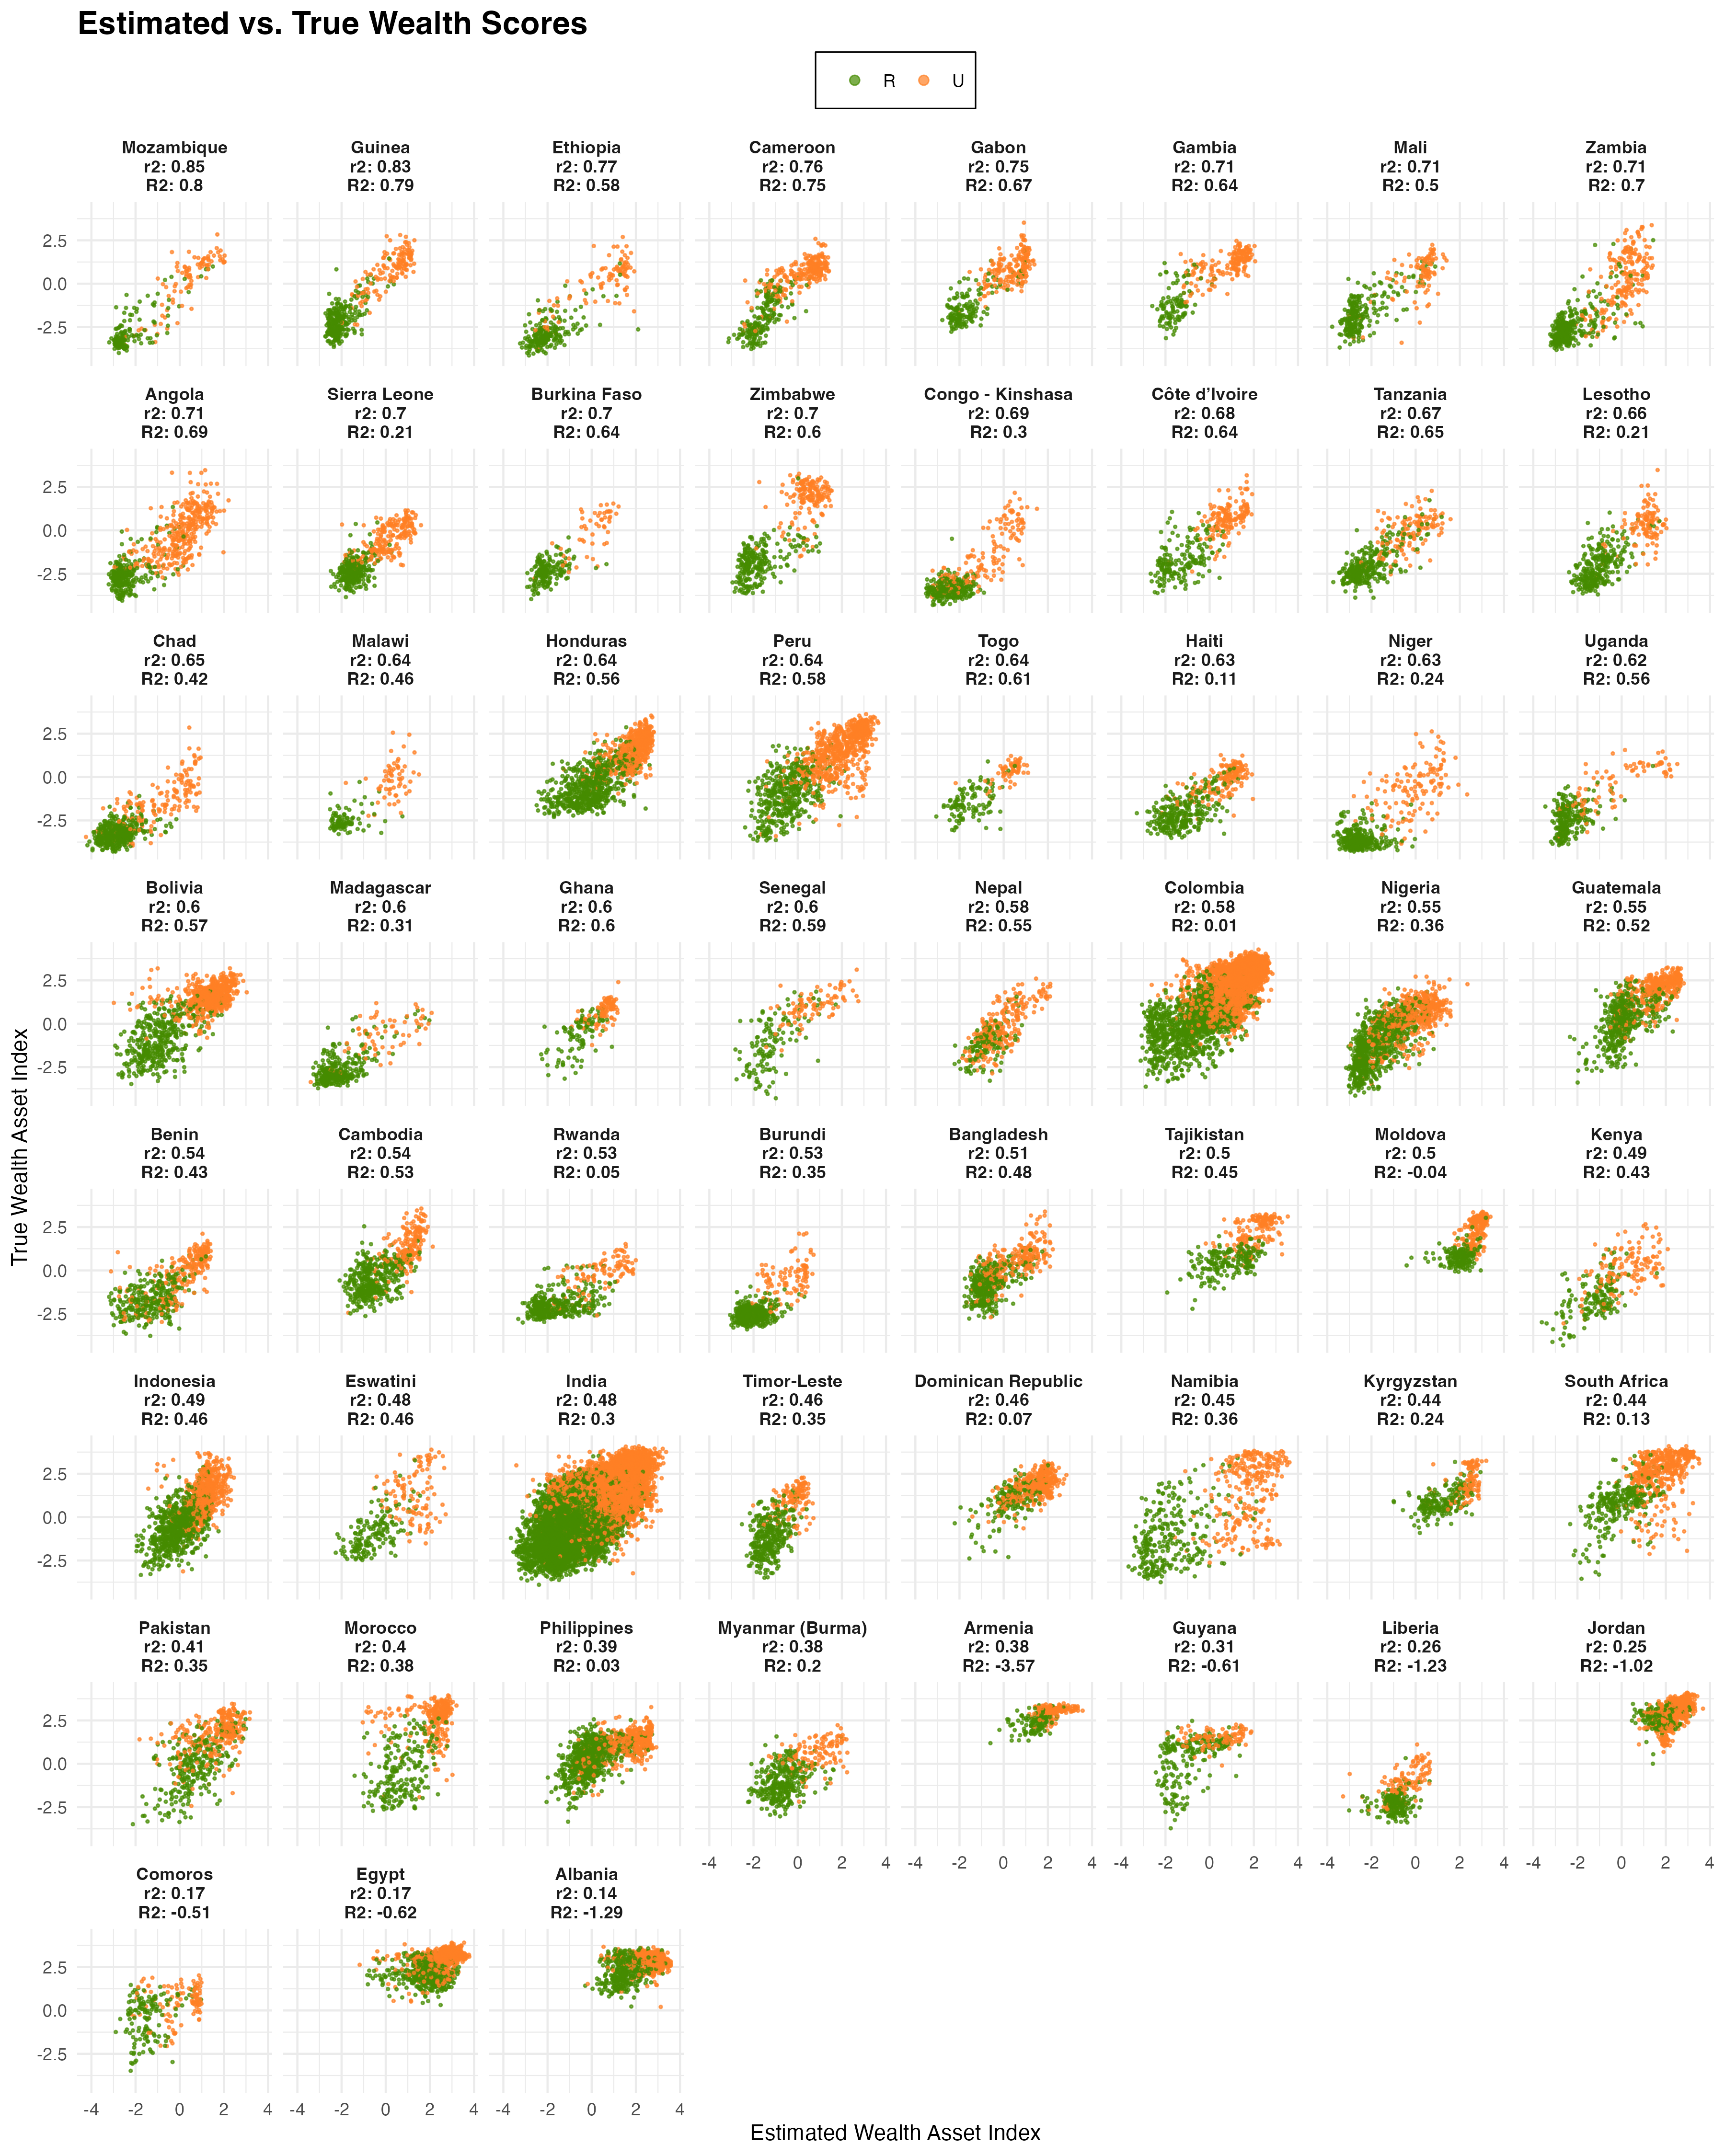
\includegraphics[width=1\textwidth]{figures/r2_scatter_eachcountry.png}
    \caption{Scatterplot between true and estimated levels of wealth for each country using survey clusters as the unit analysis. $r^2$ is the squared Pearson correlation coefficient, and $R^2$ is the coefficient of determination.}
     \label{fig:r2_scatter_eachcountry}
\end{figure}

\begin{figure}[H]
    \centering
    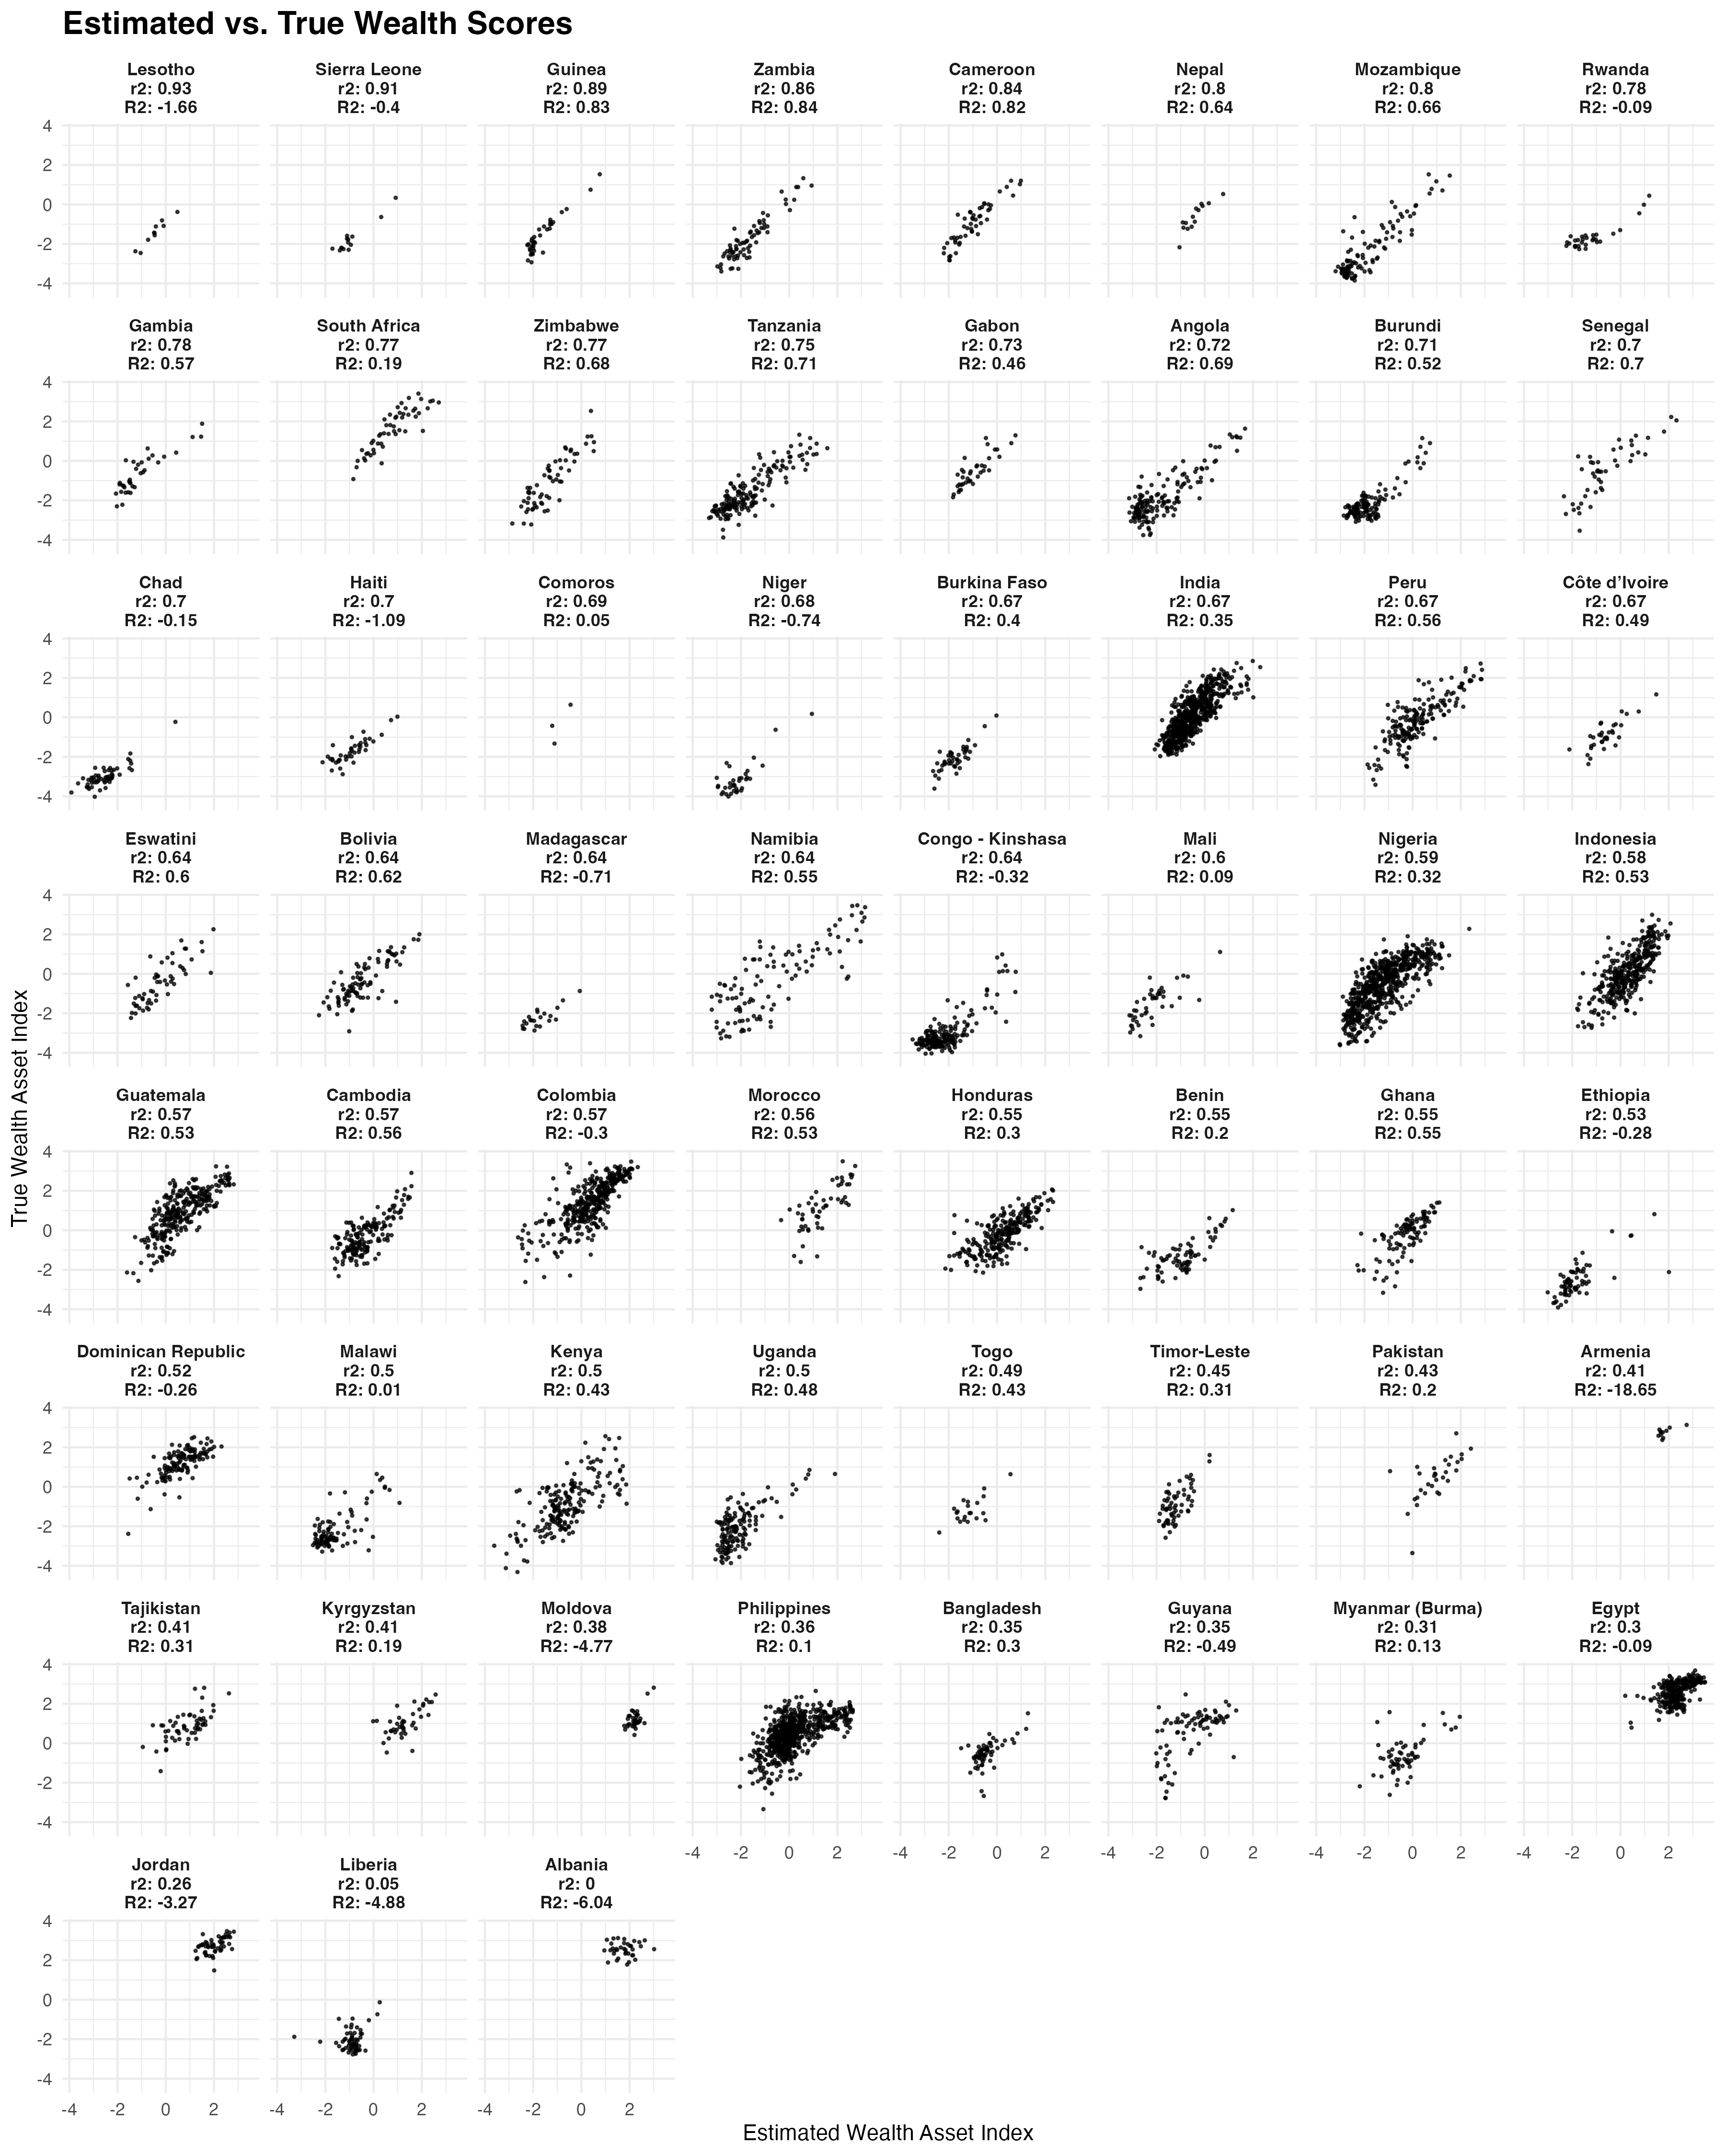
\includegraphics[width=1\textwidth]{figures/r2_scatter_eachcountry_districtagg.png}
    \caption{Scatterplot between true and estimated levels of wealth for each country when aggregating to districts. The $r^2$ is the squared Pearson correlation coefficient, and $R^2$ is the coefficient of determination.}
     \label{fig:r2_scatter_eachcountry_districtagg}
\end{figure}

% --------------------------
\newpage
\section{Estimating levels of wealth: pooled results by continent}
\label{si:r2_scatter_pooled_by_continent}

\begin{figure}[H]
    \centering
    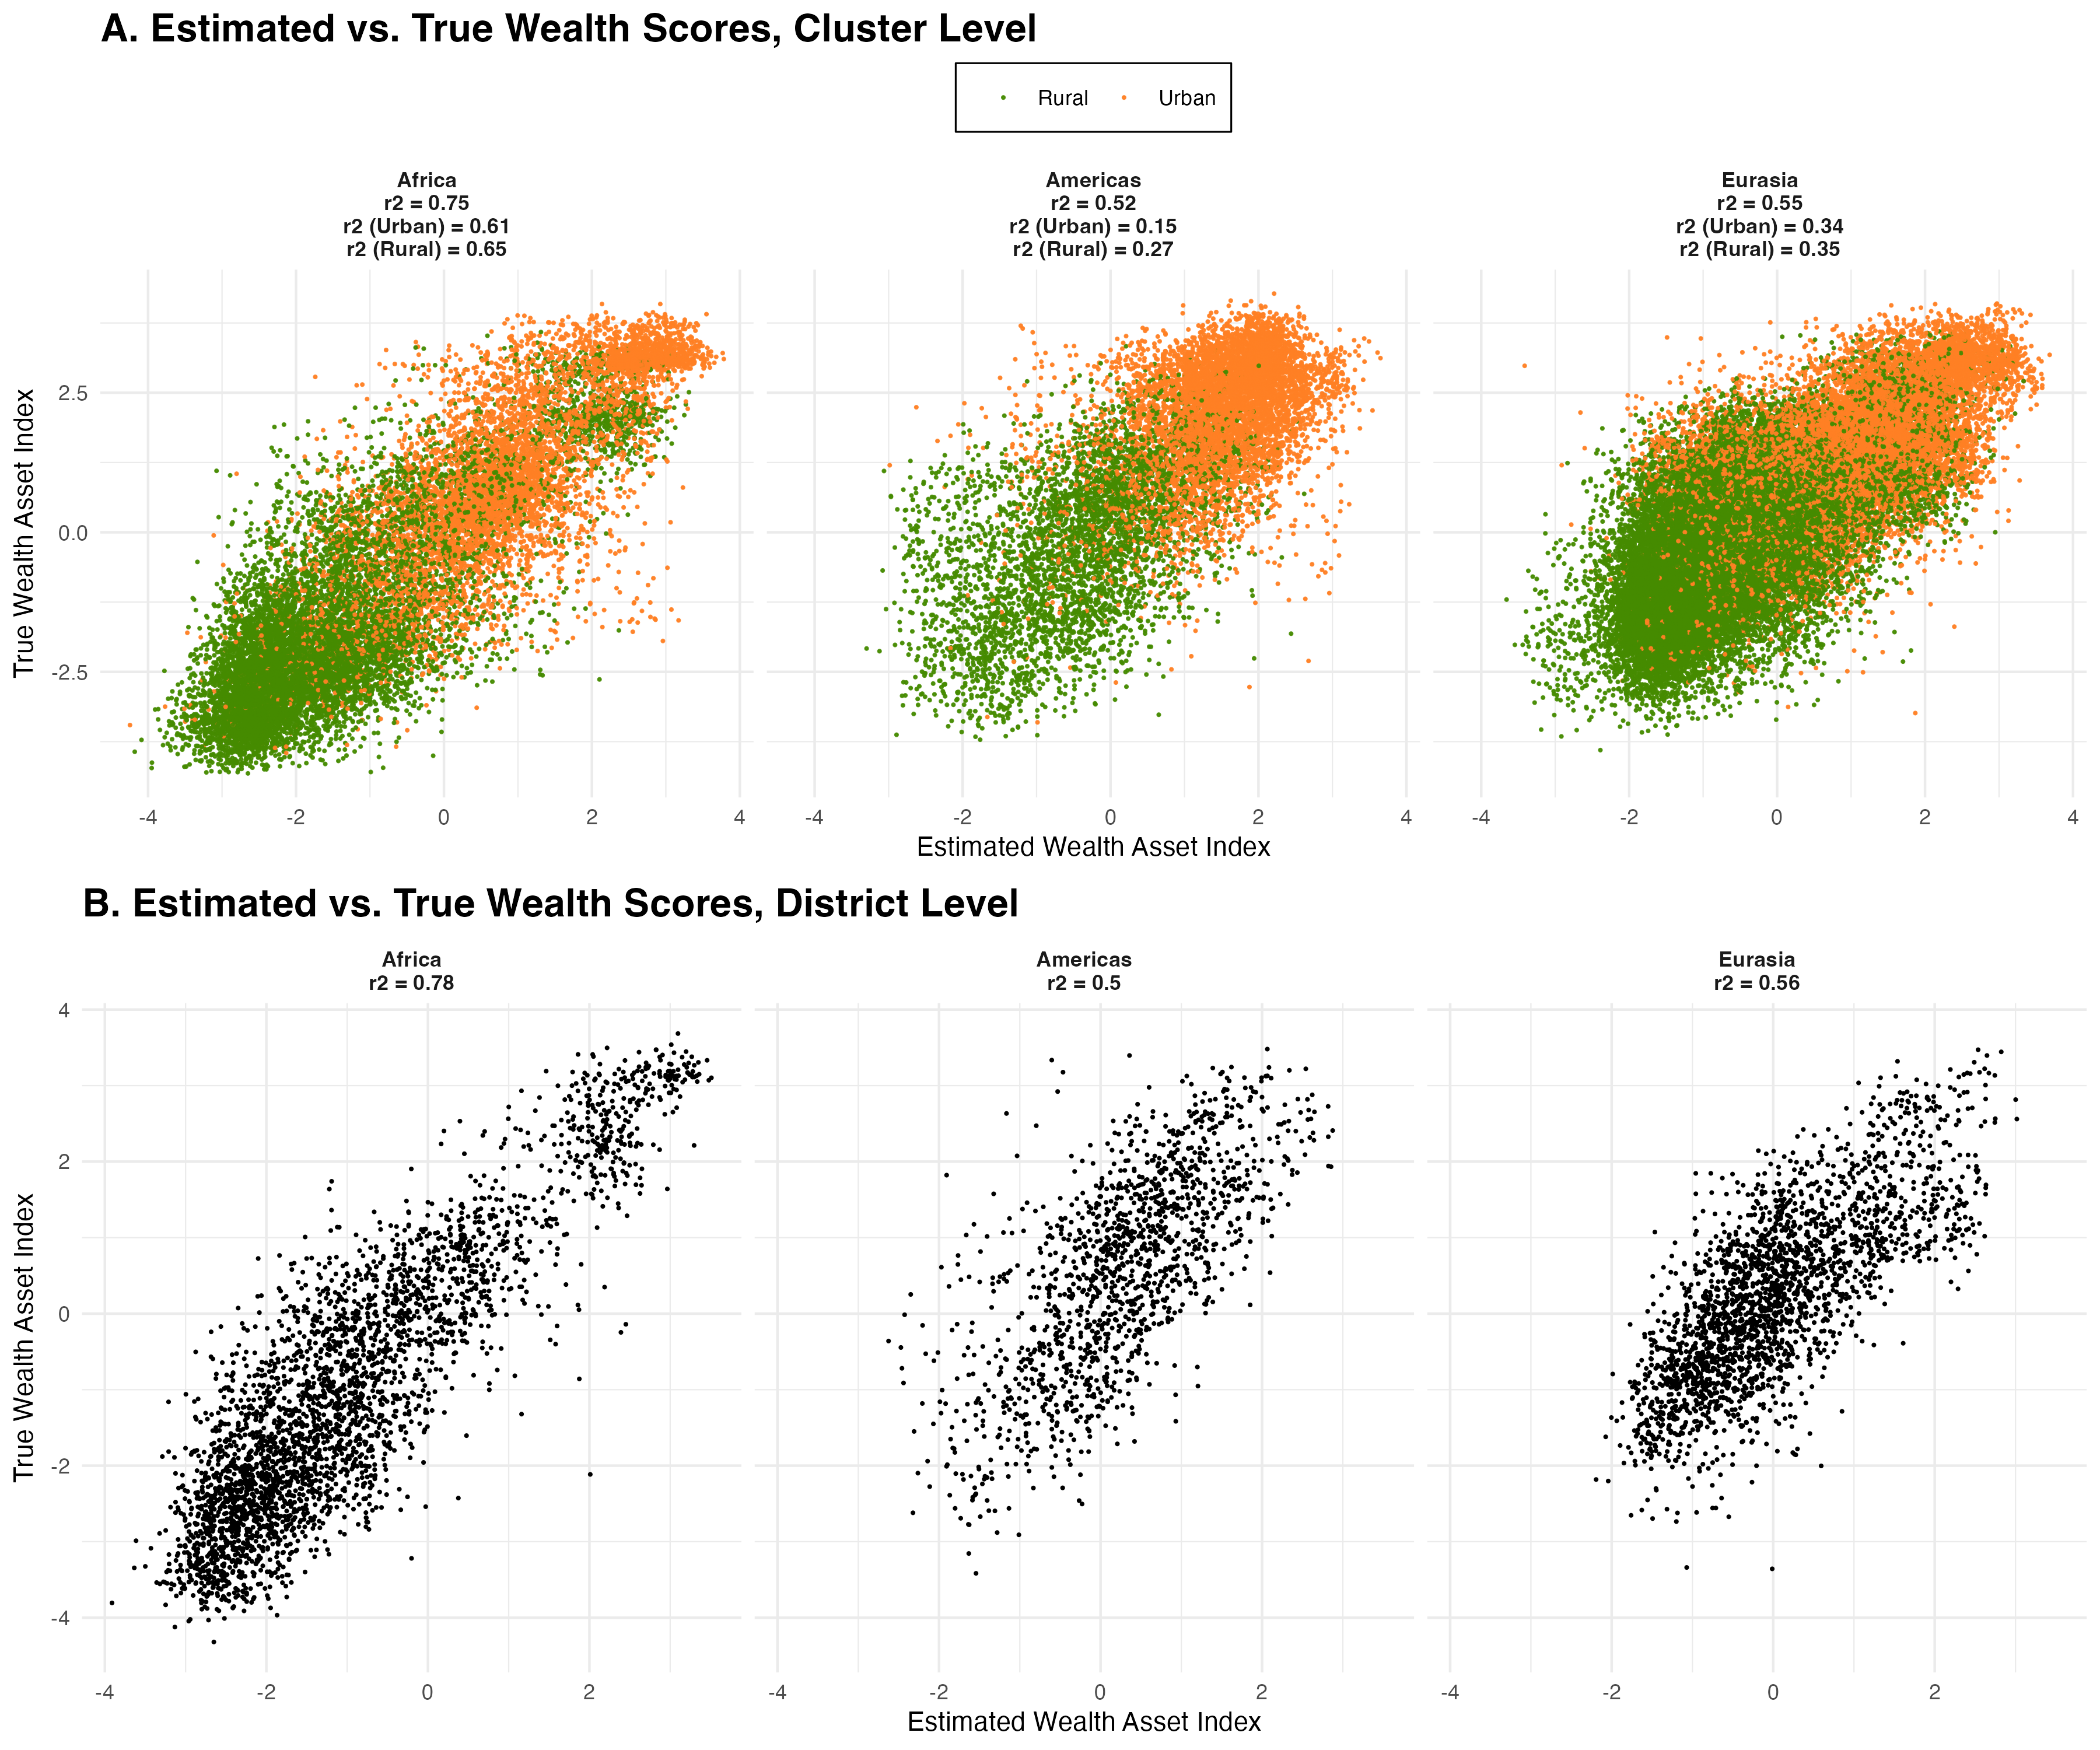
\includegraphics[width=1\textwidth]{figures/r2_scatter_pooled_by_continent.png}
    \caption{Scatterplot between true and estimated levels of wealth for each country when aggregating to districts. The $r^2$ is the squared Pearson correlation coefficient, and $R^2$ is the coefficient of determination.}
     \label{fig:r2_scatter_pooled_by_continent}
\end{figure}

% --------------------------
\newpage
\section{Model performance estimating levels of wealth for each country and feature set}
\label{si:model_perf_fs}

\begin{figure}[H]
    \centering
    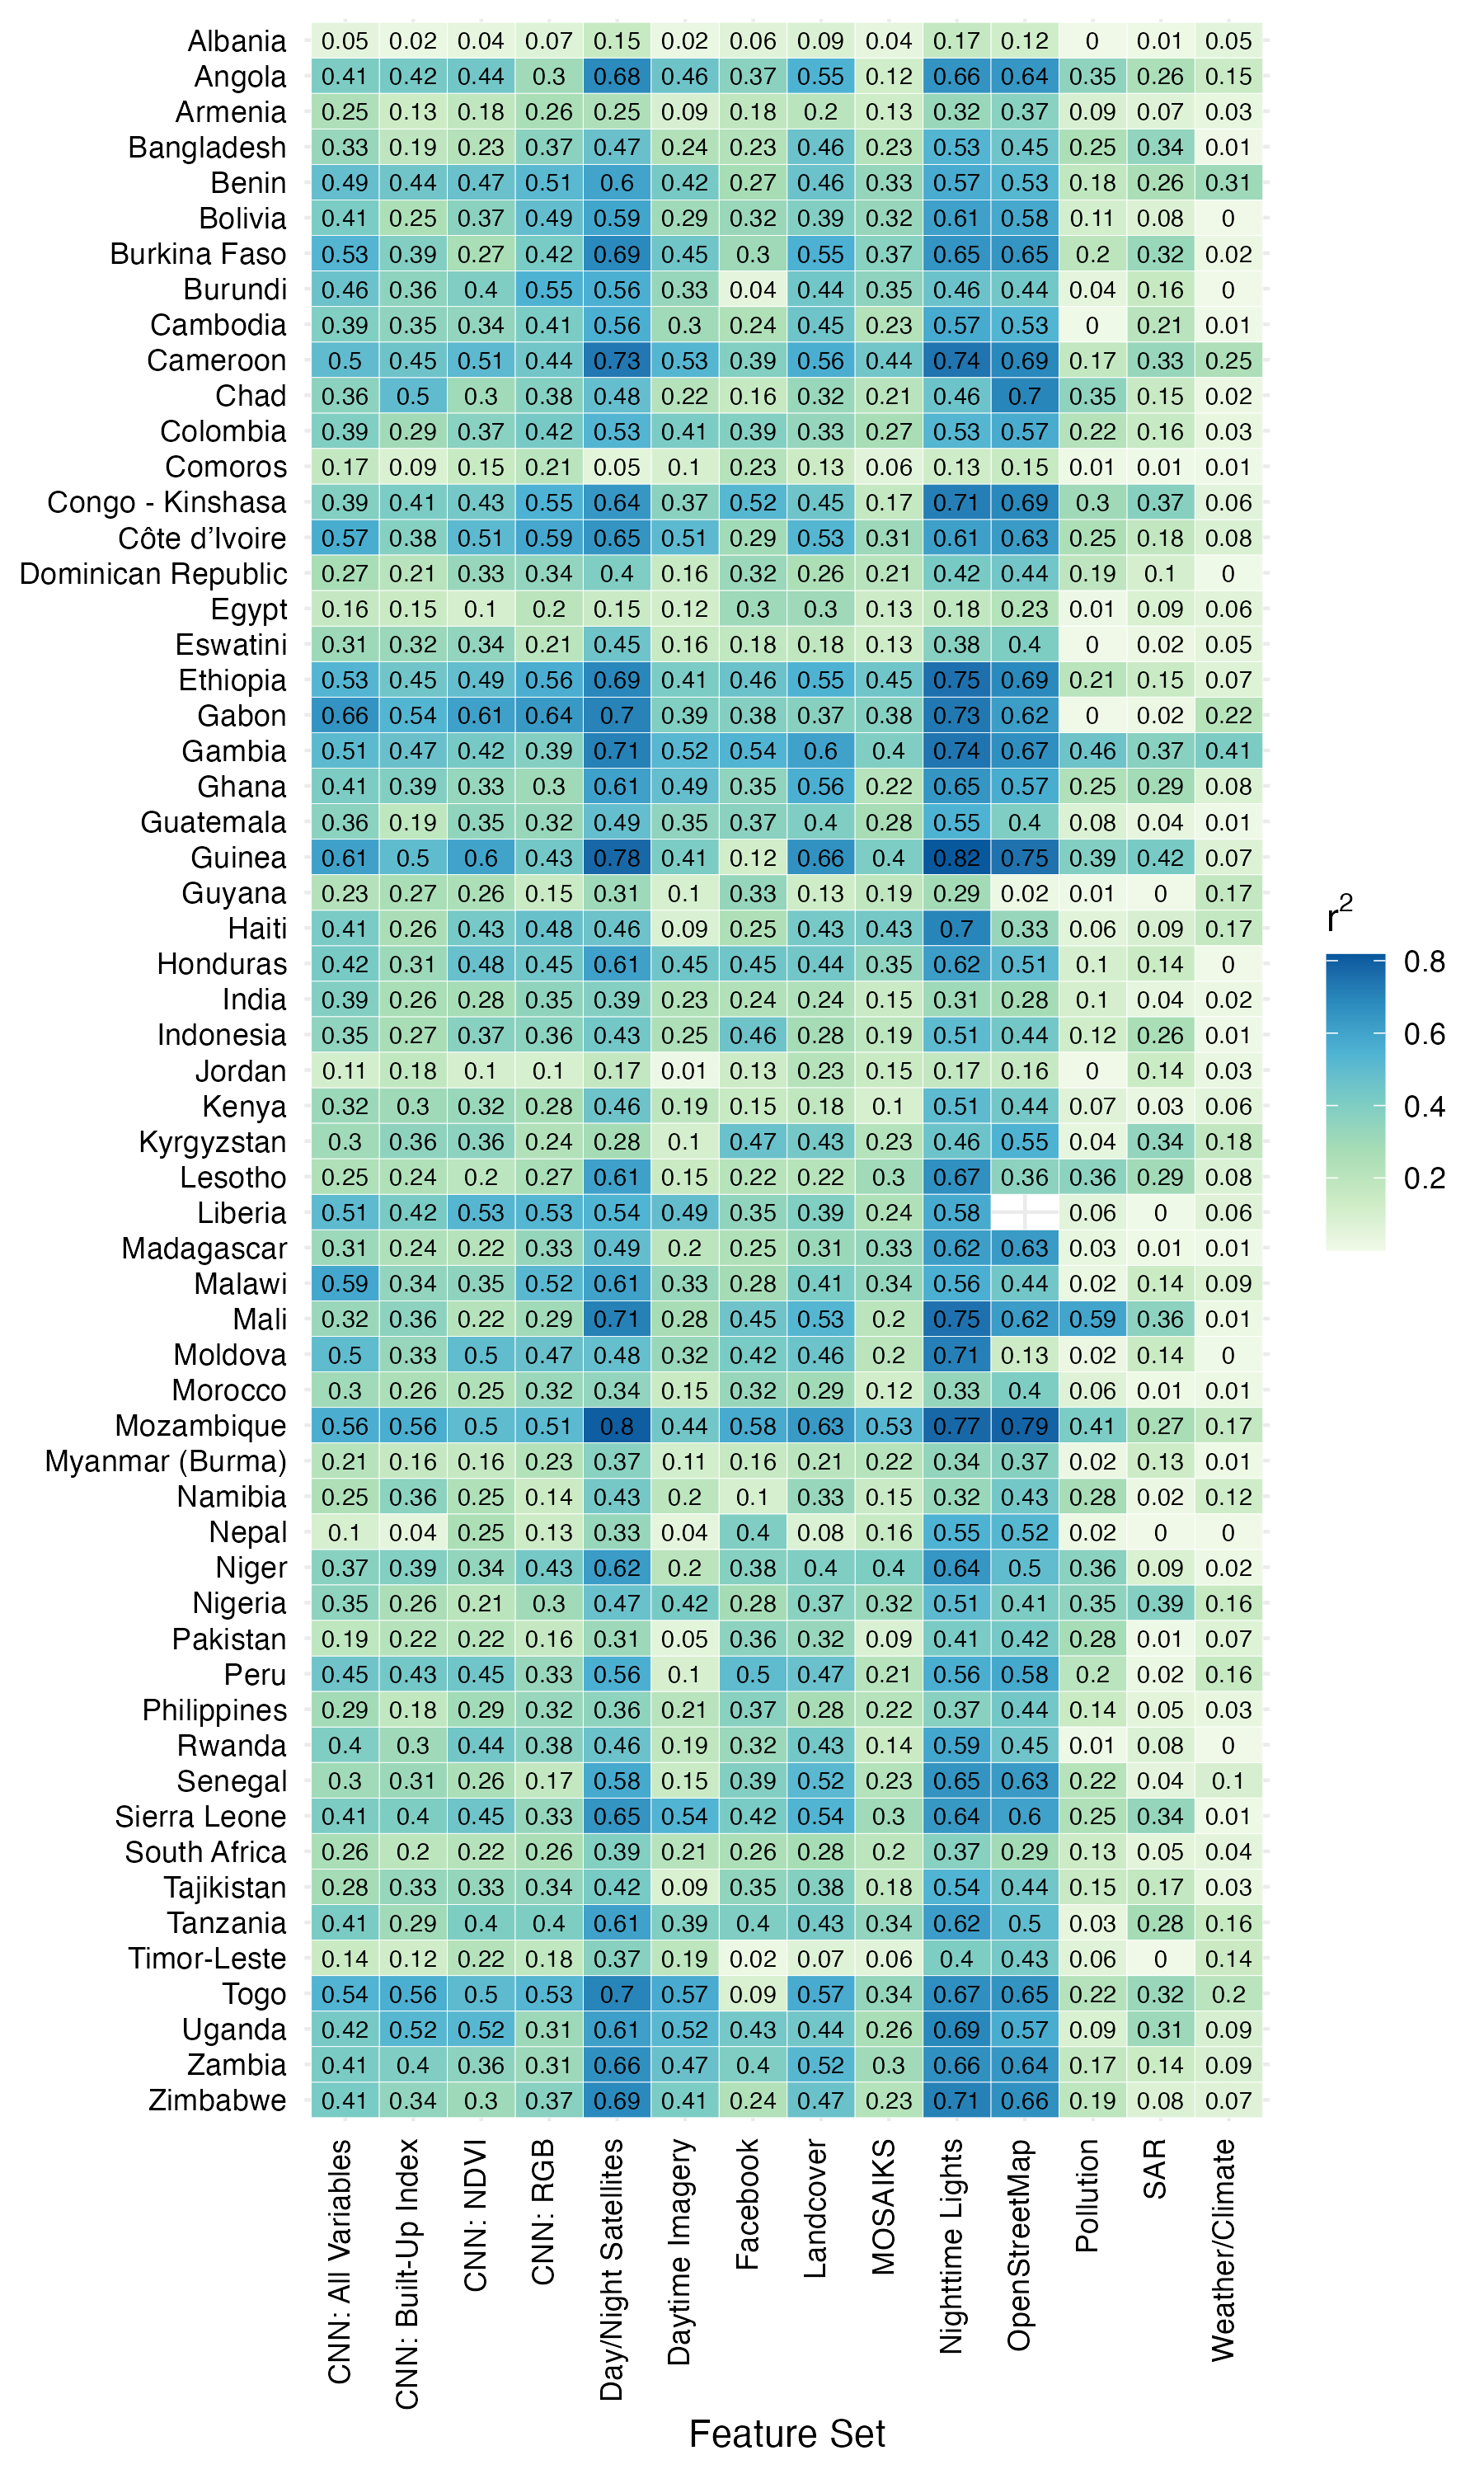
\includegraphics[width=0.8\textwidth]{figures/country_featureset_r2.png}
    \caption{Model performance estimating levels of wealth for each country and feature set}
     \label{fig:country_featureset_r2}
\end{figure}

% --------------------------
\newpage
\section{Scatterplots of true and estimated levels changes in wealth for each country}
\label{si:scatter_changes}

\begin{figure}[H]
    \centering
    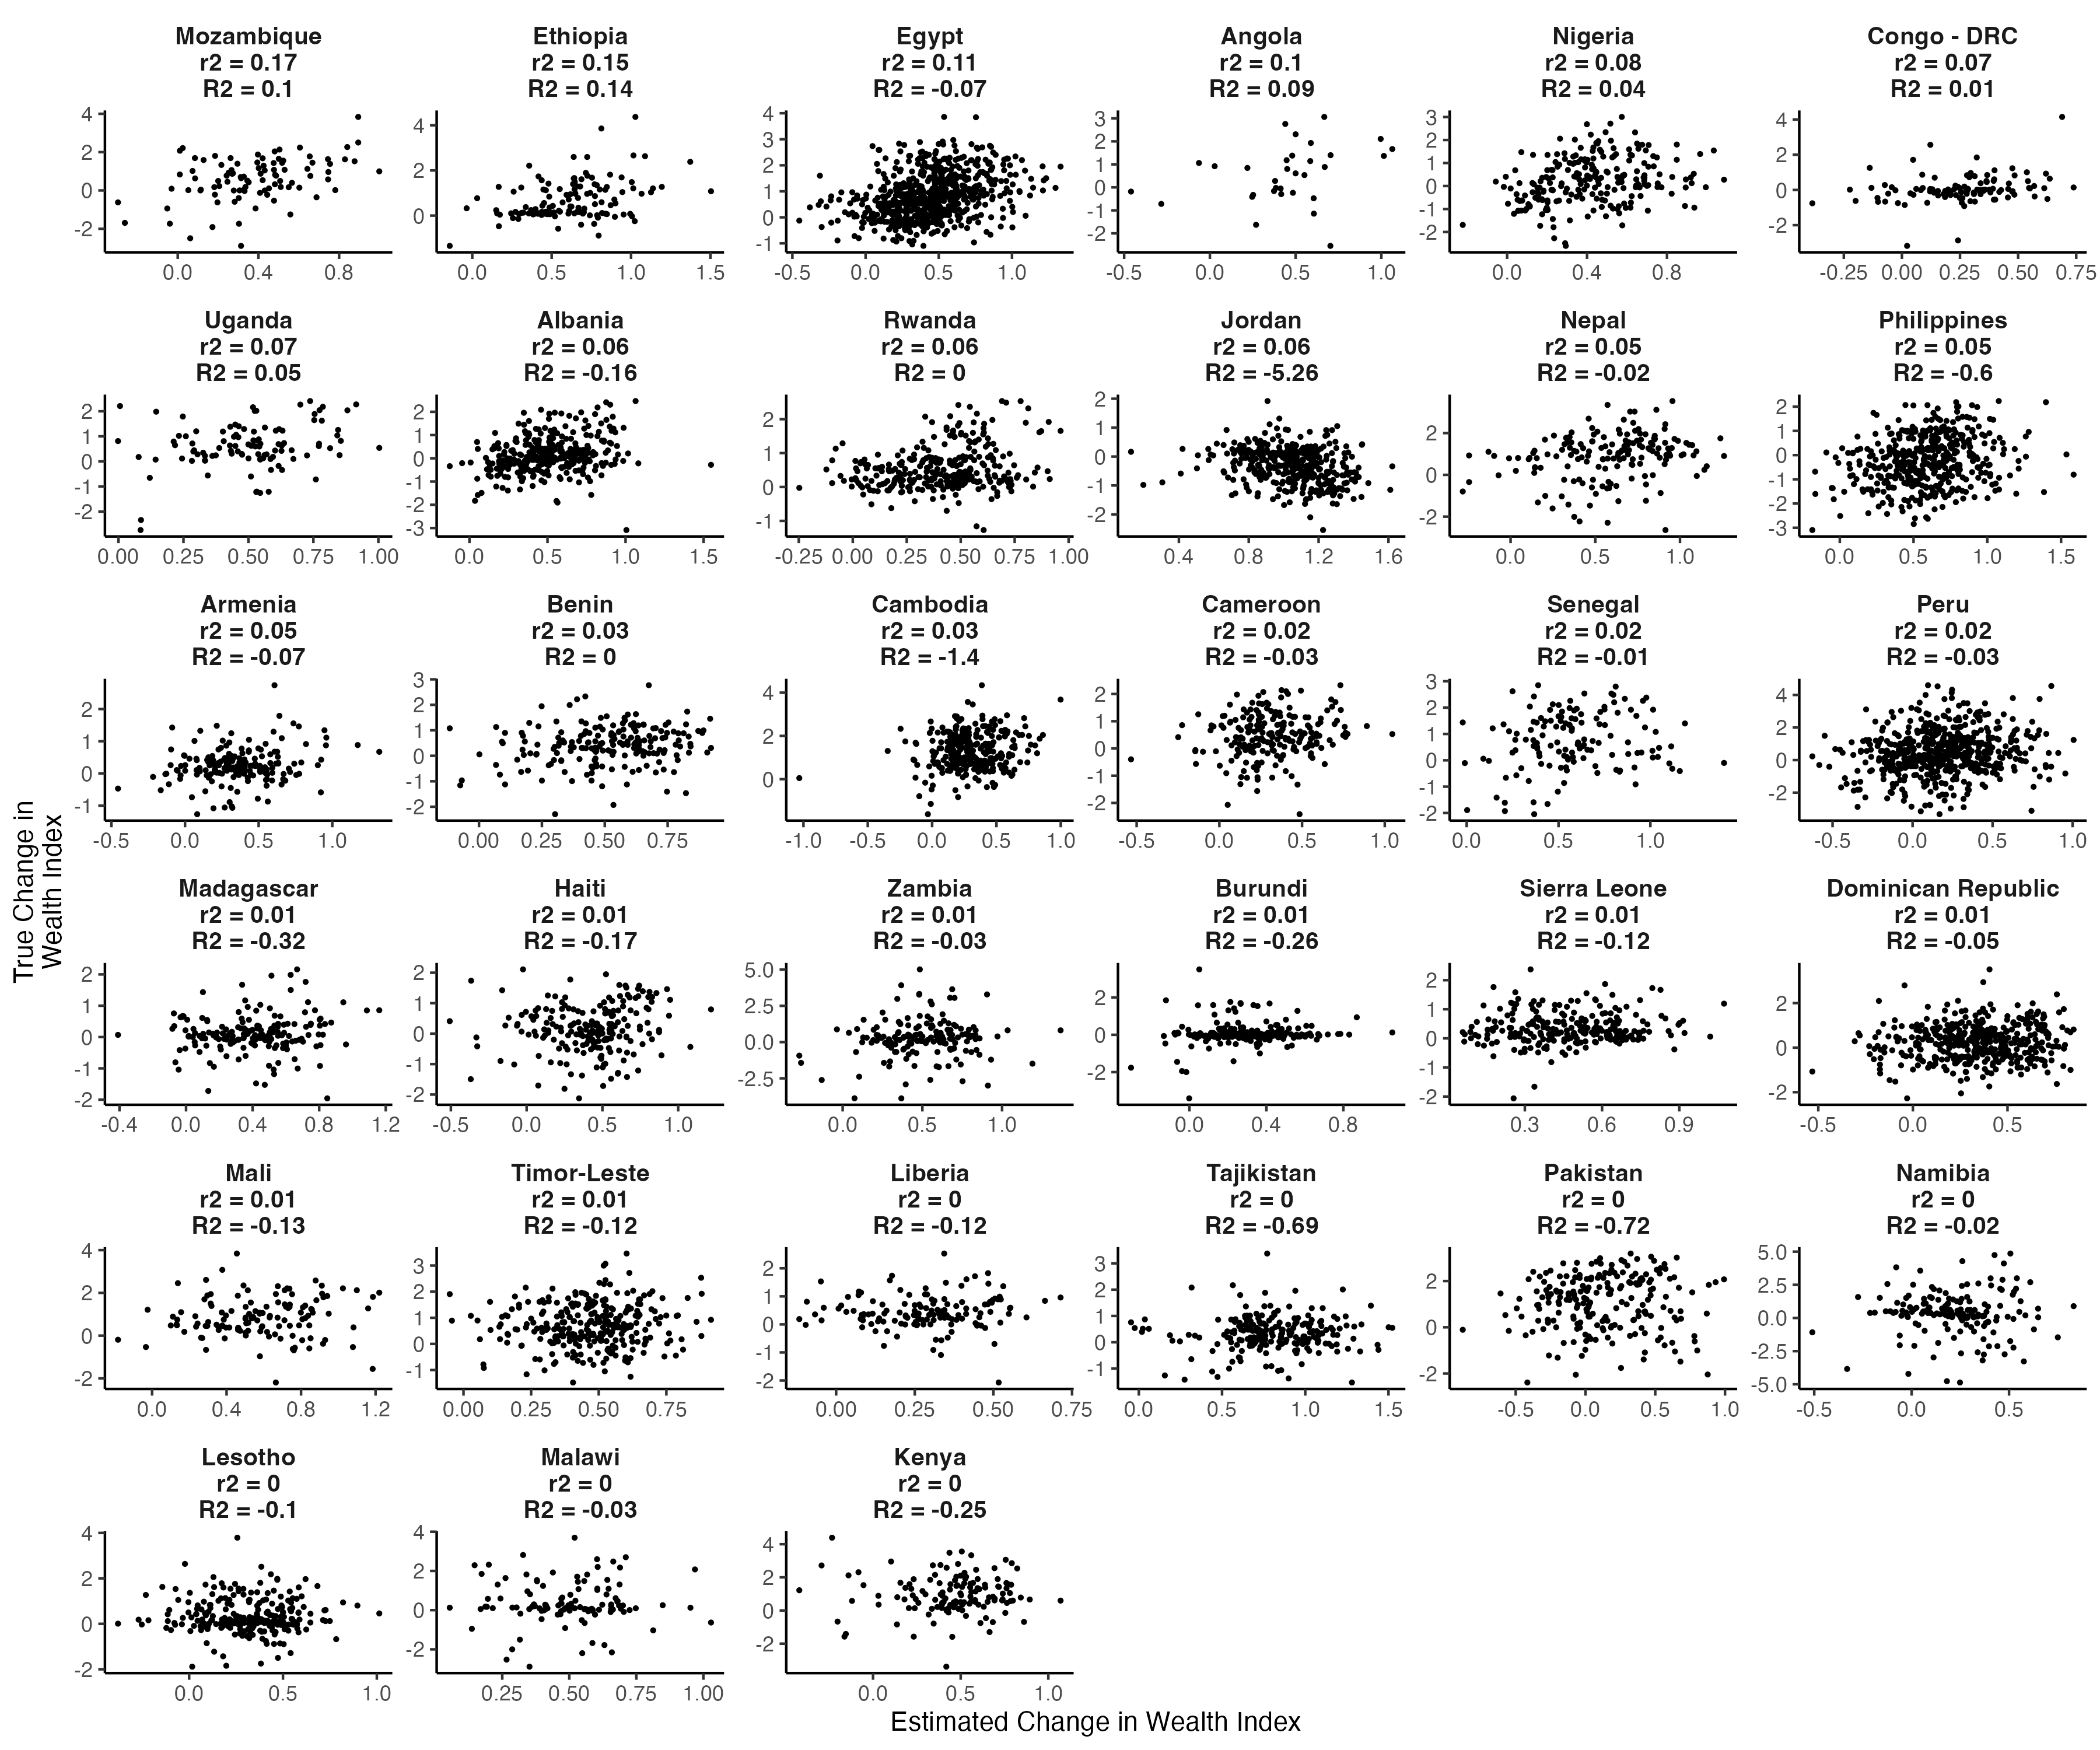
\includegraphics[width=1\textwidth]{figures/changes_scatter_cluster.png}
    \caption{Scatterplots of changes in true and estimated changes in the wealth index at the cluster level.  $r^2$ is the squared Pearson correlation coefficient, and $R^2$ is the coefficient of determination.}
     \label{fig:changes_scatter_cluster}
\end{figure}

\begin{figure}[H]
    \centering
    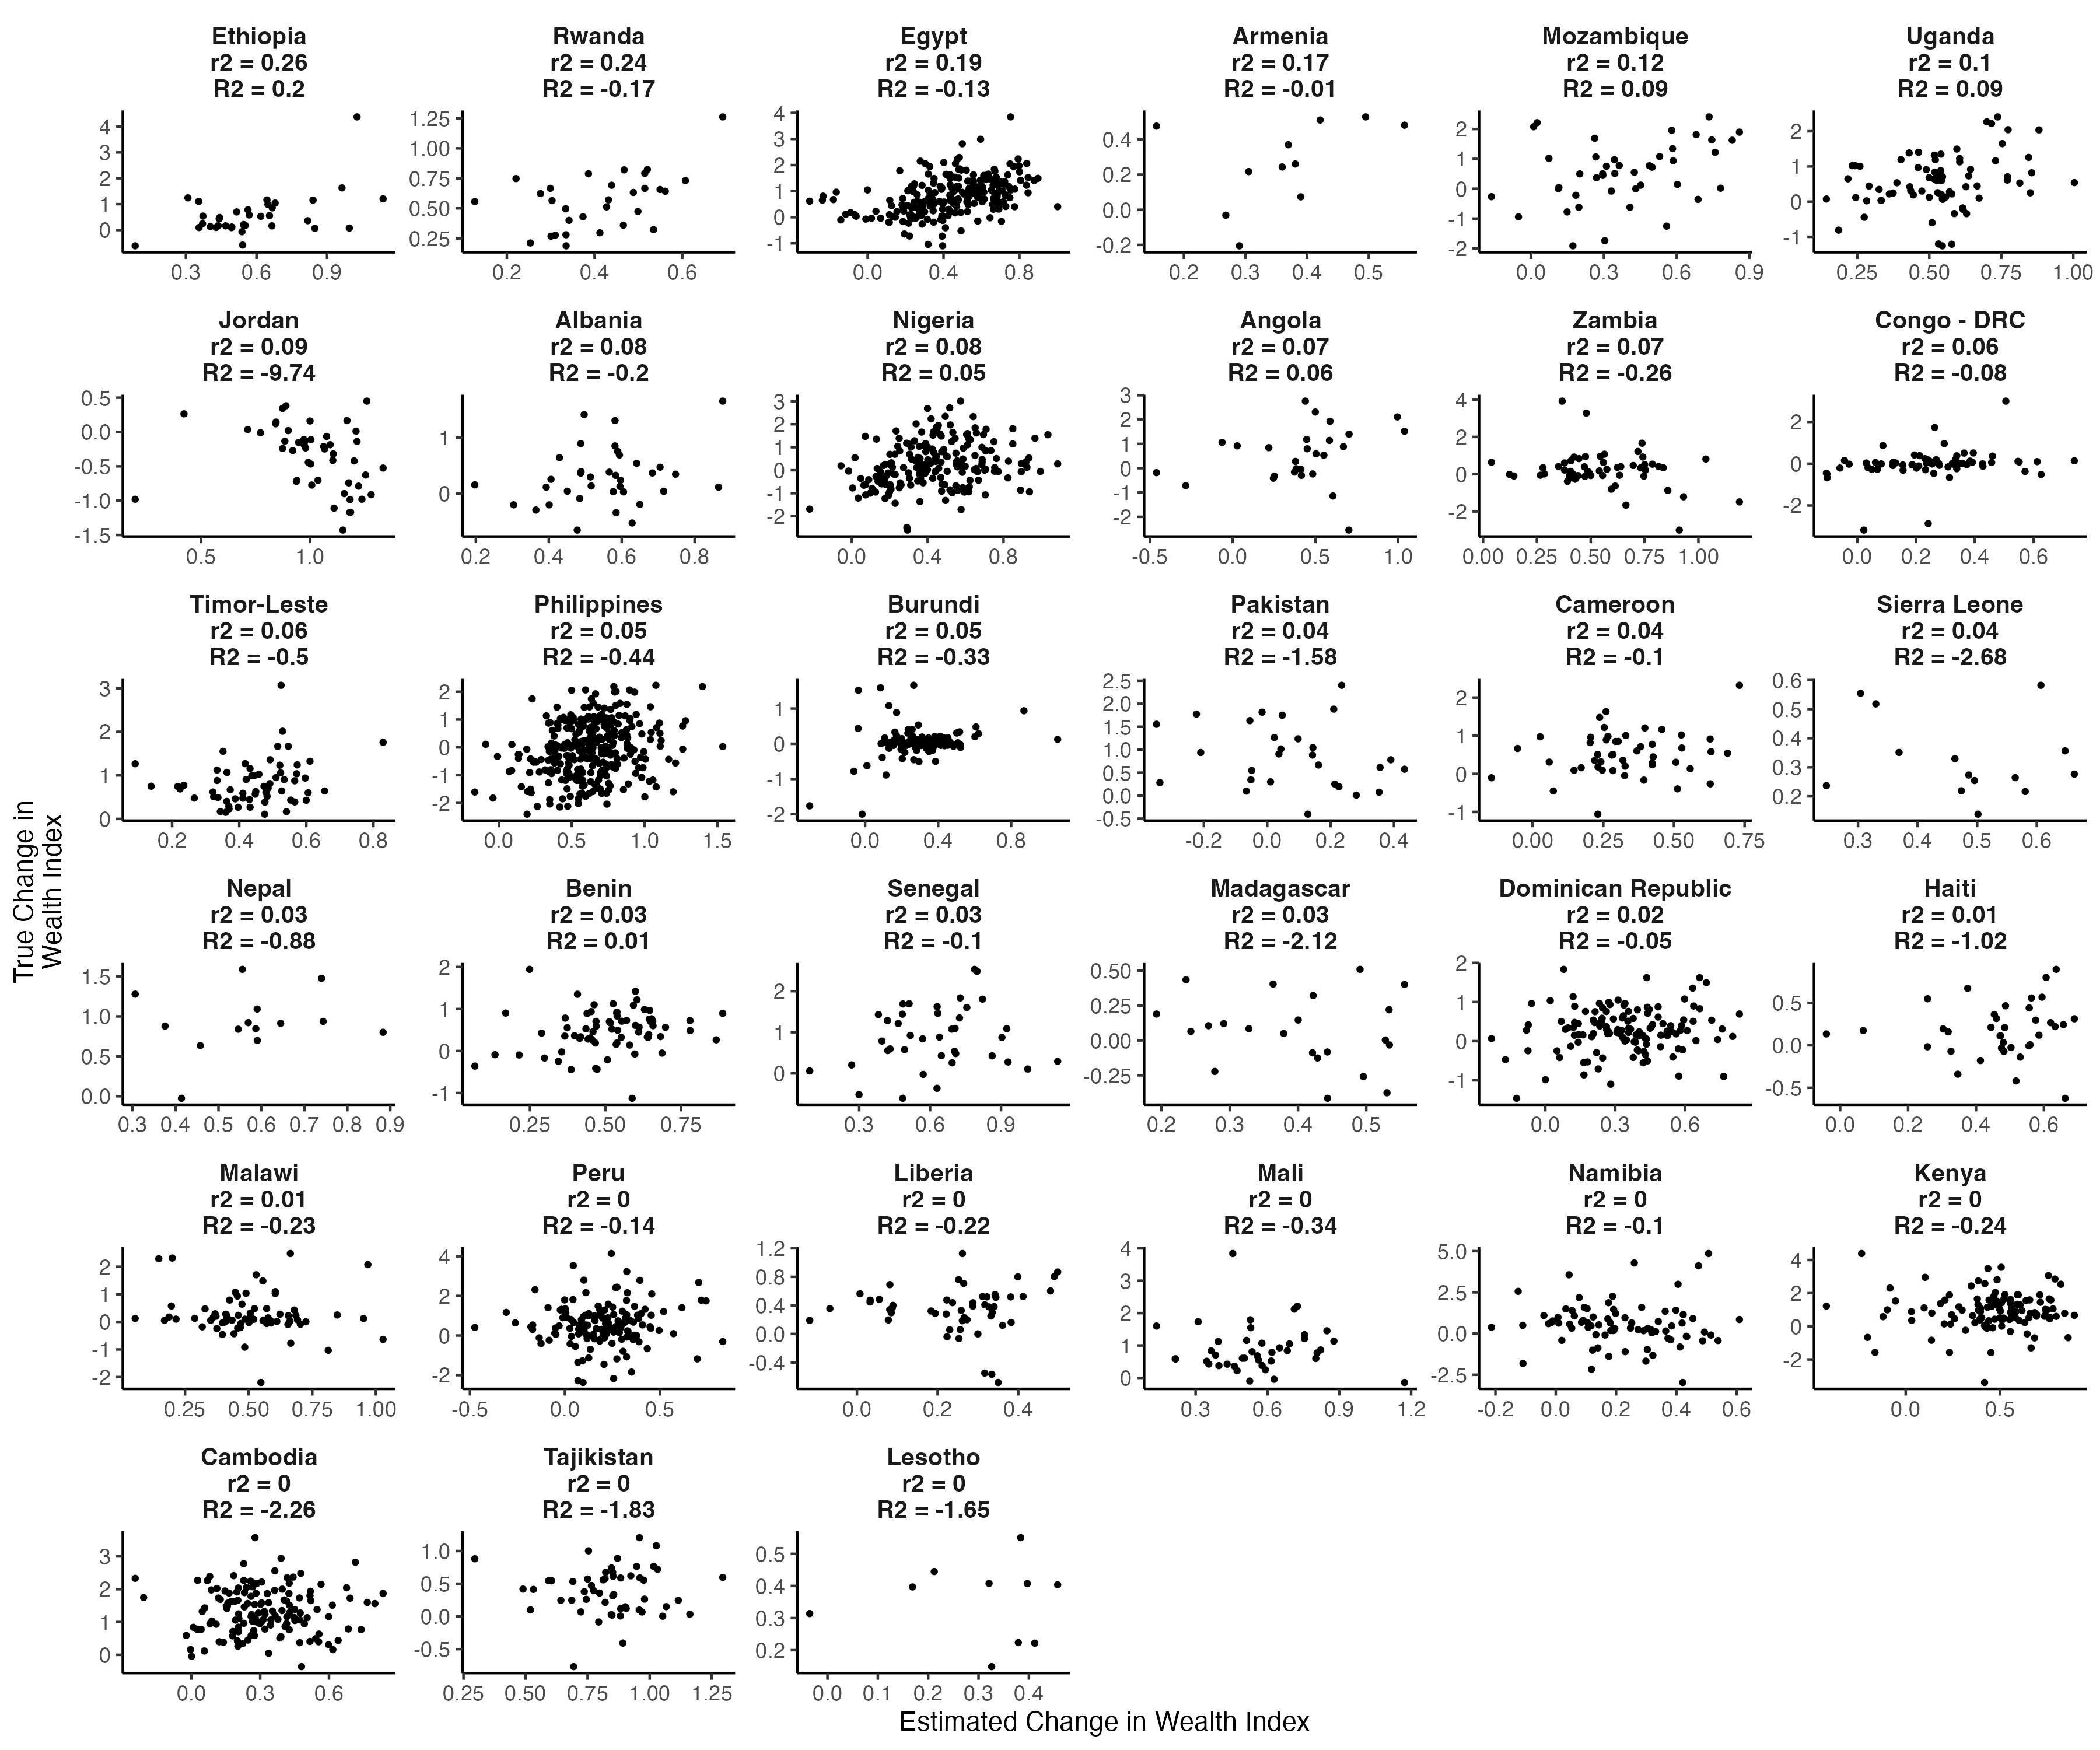
\includegraphics[width=1\textwidth]{figures/changes_scatter_adm2.png}
    \caption{Scatterplots of changes in true and estimated changes in the wealth index at the district level. \color{black} $r^2$ is the squared Pearson correlation coefficient, and $R^2$ is the coefficient of determination.}
     \label{fig:changes_scatter_adm2}
\end{figure}

% --------------------------

\newpage
\section{Explain variation in error}
\label{si:expl_error_var}

\singlespacing
\begin{table}[H]
\small
\caption{Explaining error (absolute value of true minus predicted wealth) based on select factors}
\label{tab:explain_error_levels_lm}
\centering

% Table created by stargazer v.5.2.3 by Marek Hlavac, Social Policy Institute. E-mail: marek.hlavac at gmail.com
% Date and time: Tue, Nov 07, 2023 - 14:31:46
\begin{tabular}{@{\extracolsep{5pt}}lc} 
\\[-1.8ex]\hline 
\hline \\[-1.8ex] 
 & \multicolumn{1}{c}{\textit{Dependent variable:}} \\ 
\cline{2-2} 
\\[-1.8ex] & Absolute value of difference in true and estimated wealth \\ 
\hline \\[-1.8ex] 
 Nighttime lights & $-$0.126$^{***}$ \\ 
  & (0.003) \\ 
  & \\ 
 Urban & 0.187$^{***}$ \\ 
  & (0.007) \\ 
  & \\ 
 Lower middle income & 0.095$^{***}$ \\ 
  & (0.011) \\ 
  & \\ 
 Upper middle income & 0.264$^{***}$ \\ 
  & (0.013) \\ 
  & \\ 
 Americas & 0.062$^{***}$ \\ 
  & (0.011) \\ 
  & \\ 
 Eurasia & 0.036$^{***}$ \\ 
  & (0.008) \\ 
  & \\ 
 Constant & 0.785$^{***}$ \\ 
  & (0.009) \\ 
  & \\ 
\hline \\[-1.8ex] 
Observations & 63,854 \\ 
R$^{2}$ & 0.035 \\ 
Adjusted R$^{2}$ & 0.035 \\ 
\hline 
\hline \\[-1.8ex] 
\textit{Note:}  & \multicolumn{1}{r}{$^{*}$p$<$0.1; $^{**}$p$<$0.05; $^{***}$p$<$0.01} \\ 
\end{tabular} 

\end{table}
\normalsize
\doublespacing

\singlespacing
\begin{table}[H]
\small
\caption{Explaining error (absolute value of true minus predicted wealth) based on select factors}
\label{tab:explain_error_changes_lm}
\centering

% Table created by stargazer v.5.2.3 by Marek Hlavac, Social Policy Institute. E-mail: marek.hlavac at gmail.com
% Date and time: Tue, Nov 07, 2023 - 14:32:22
\begin{tabular}{@{\extracolsep{5pt}}lc} 
\\[-1.8ex]\hline 
\hline \\[-1.8ex] 
 & \multicolumn{1}{c}{\textit{Dependent variable:}} \\ 
\cline{2-2} 
\\[-1.8ex] & Absolute value of difference in change in true and estimated wealth \\ 
\hline \\[-1.8ex] 
 Change in nighttime lights, absolute value & 0.016$^{***}$ \\ 
  & (0.001) \\ 
  & \\ 
 Urban (baseline) & 0.169$^{***}$ \\ 
  & (0.015) \\ 
  & \\ 
 Lower middle income & 0.142$^{***}$ \\ 
  & (0.021) \\ 
  & \\ 
 Upper middle income & 0.158$^{***}$ \\ 
  & (0.030) \\ 
  & \\ 
 Americas & 0.094$^{***}$ \\ 
  & (0.029) \\ 
  & \\ 
 Eurasia & 0.191$^{***}$ \\ 
  & (0.020) \\ 
  & \\ 
 Constant & 0.409$^{***}$ \\ 
  & (0.017) \\ 
  & \\ 
\hline \\[-1.8ex] 
Observations & 7,714 \\ 
R$^{2}$ & 0.094 \\ 
Adjusted R$^{2}$ & 0.094 \\ 
\hline 
\hline \\[-1.8ex] 
\textit{Note:}  & \multicolumn{1}{r}{$^{*}$p$<$0.1; $^{**}$p$<$0.05; $^{***}$p$<$0.01} \\ 
\end{tabular} 

\end{table}
\normalsize
\doublespacing

\begin{figure}[H]
    \centering
    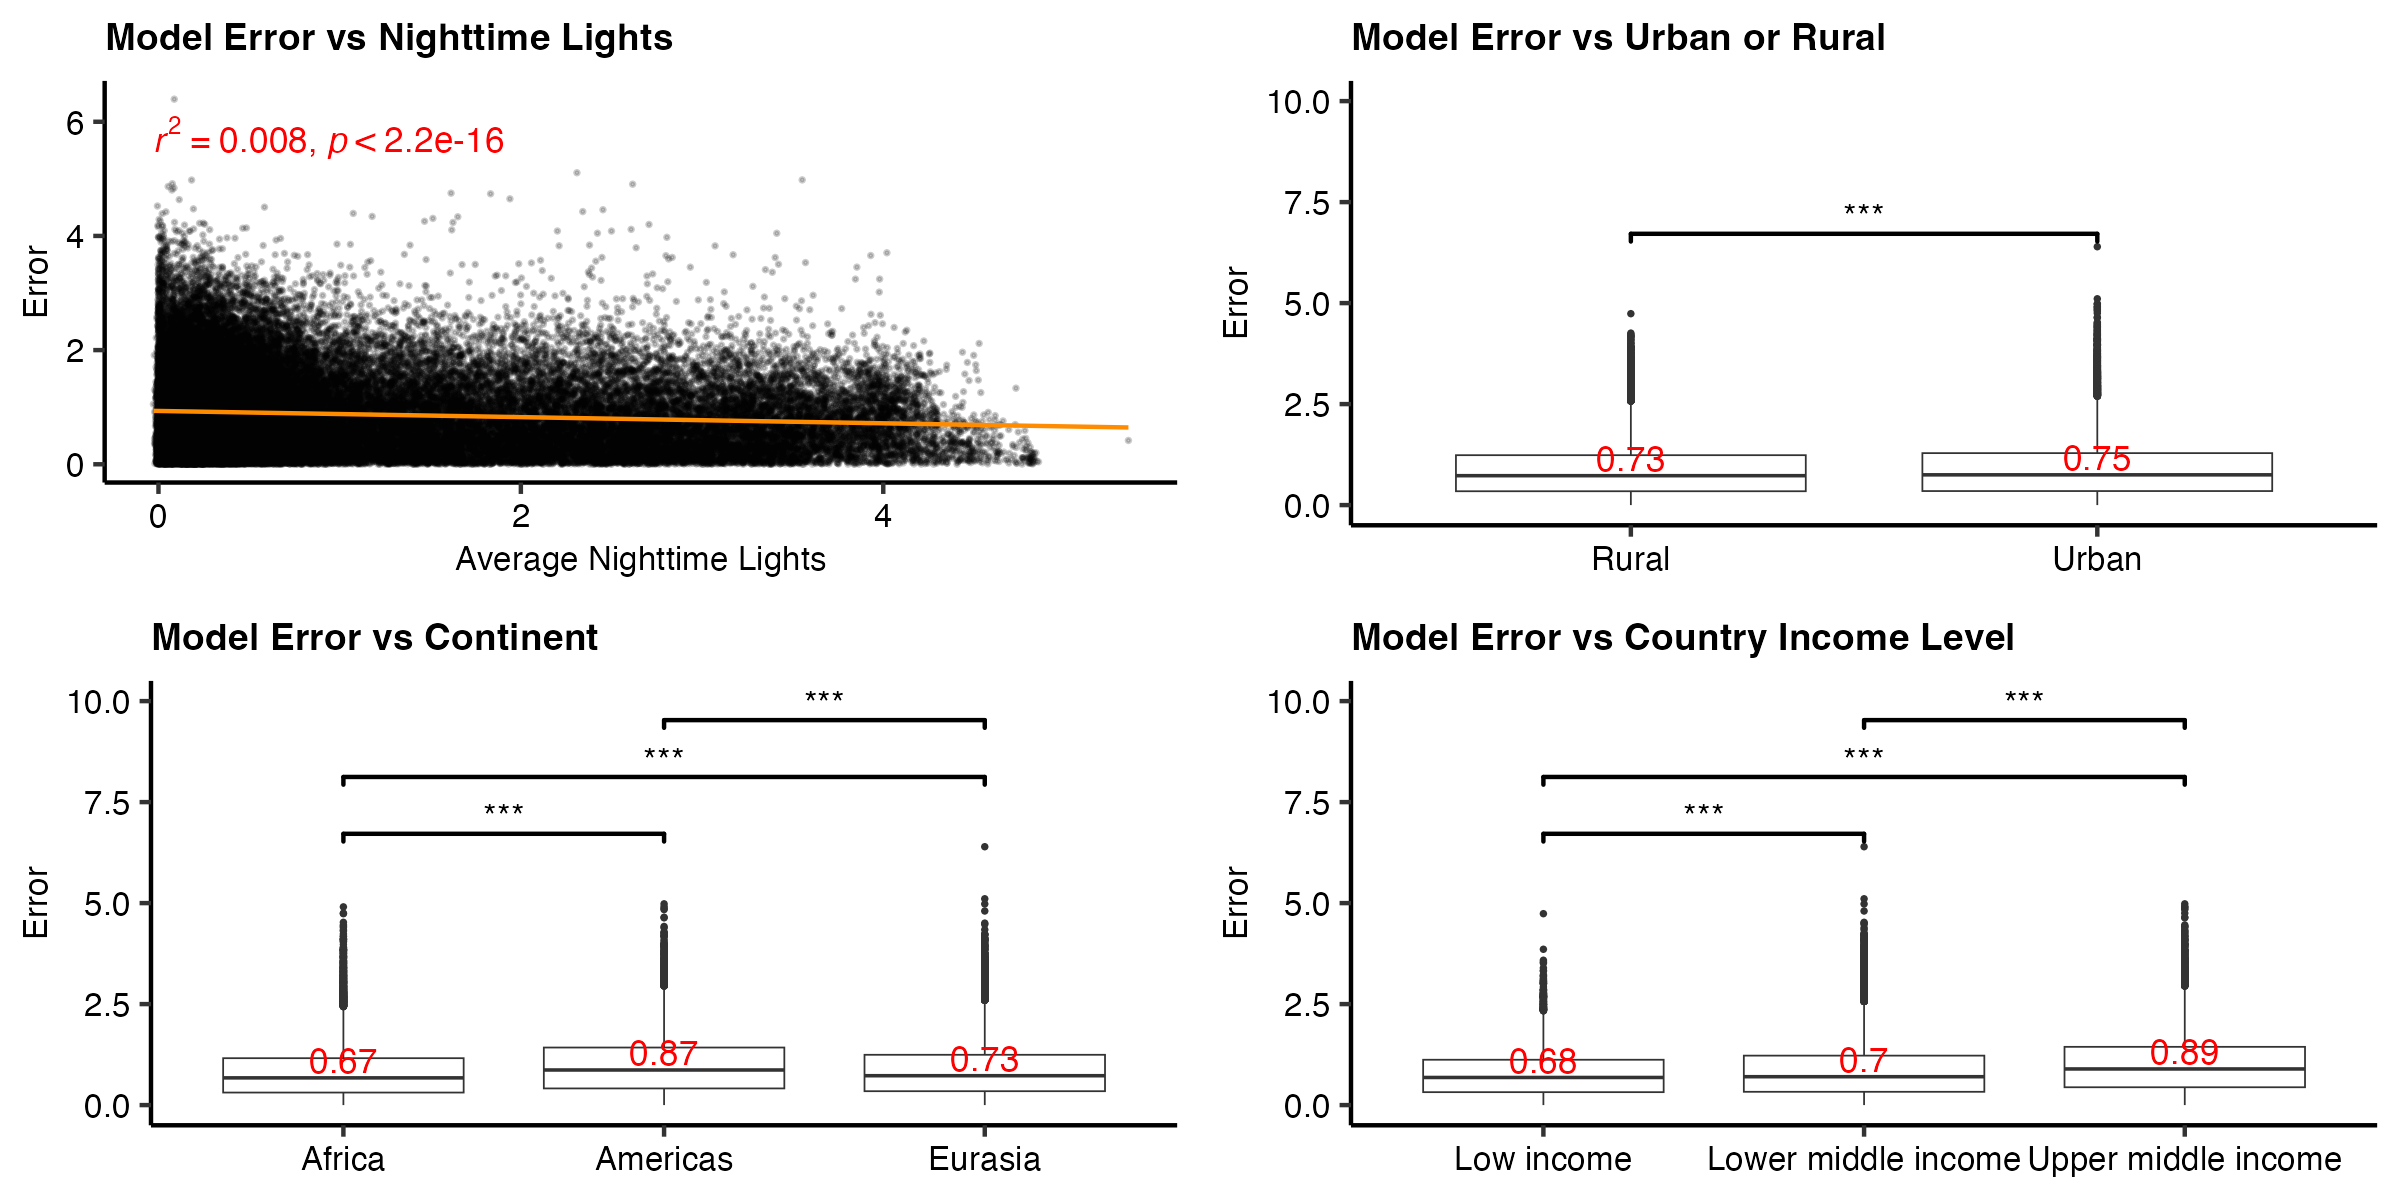
\includegraphics[width=0.8\textwidth]{figures/explain_error_levels.png}
    \caption{Explain error: levels. The boxplots include: center line, median; box limits, upper and lower quartiles; whiskers, 1.5x interquartile range; points beyond whiskers, outliers. {$^{*}$p$<$0.1; $^{**}$p$<$0.05; $^{***}$p$<$0.01}}
     \label{fig:explain_error_levels}
\end{figure}

\begin{figure}[H]
    \centering
    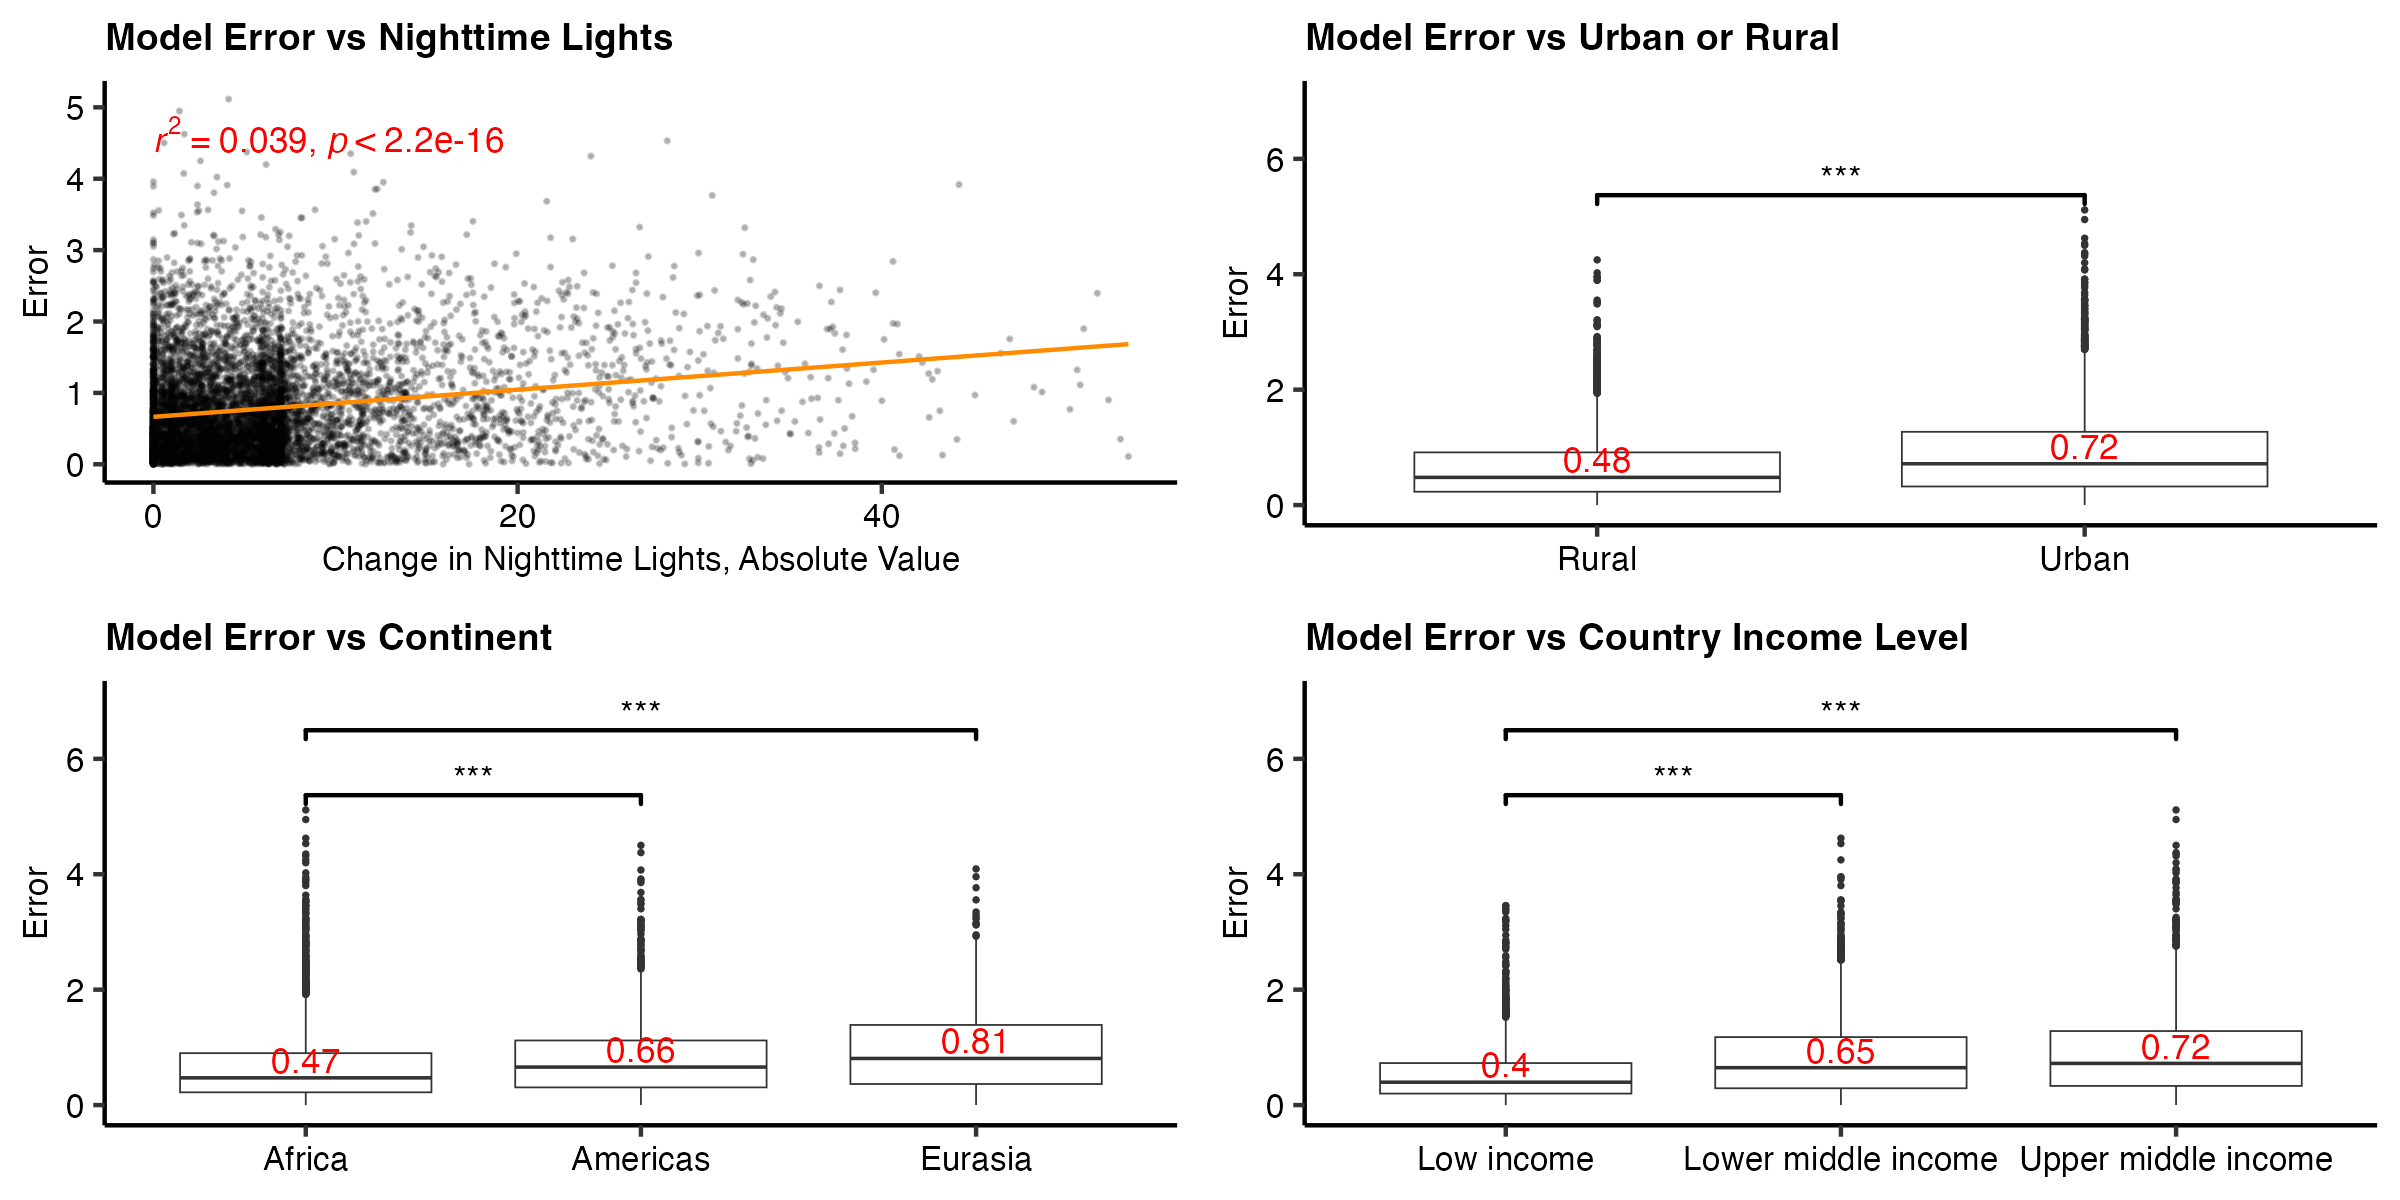
\includegraphics[width=0.8\textwidth]{figures/explain_error_changes.png}
    \caption{Explain error: changes. The boxplots include: center line, median; box limits, upper and lower quartiles; whiskers, 1.5x interquartile range; points beyond whiskers, outliers. {$^{*}$p$<$0.1; $^{**}$p$<$0.05; $^{***}$p$<$0.01}}
     \label{fig:explain_error_changes}
\end{figure}

% --------------------------
\newpage
\section{Application: Estimating Wealth in Different Years using First Administrative Division}
\label{si:policy_exp_nigeria_gadm_1}

\begin{figure}[H]
    \centering
    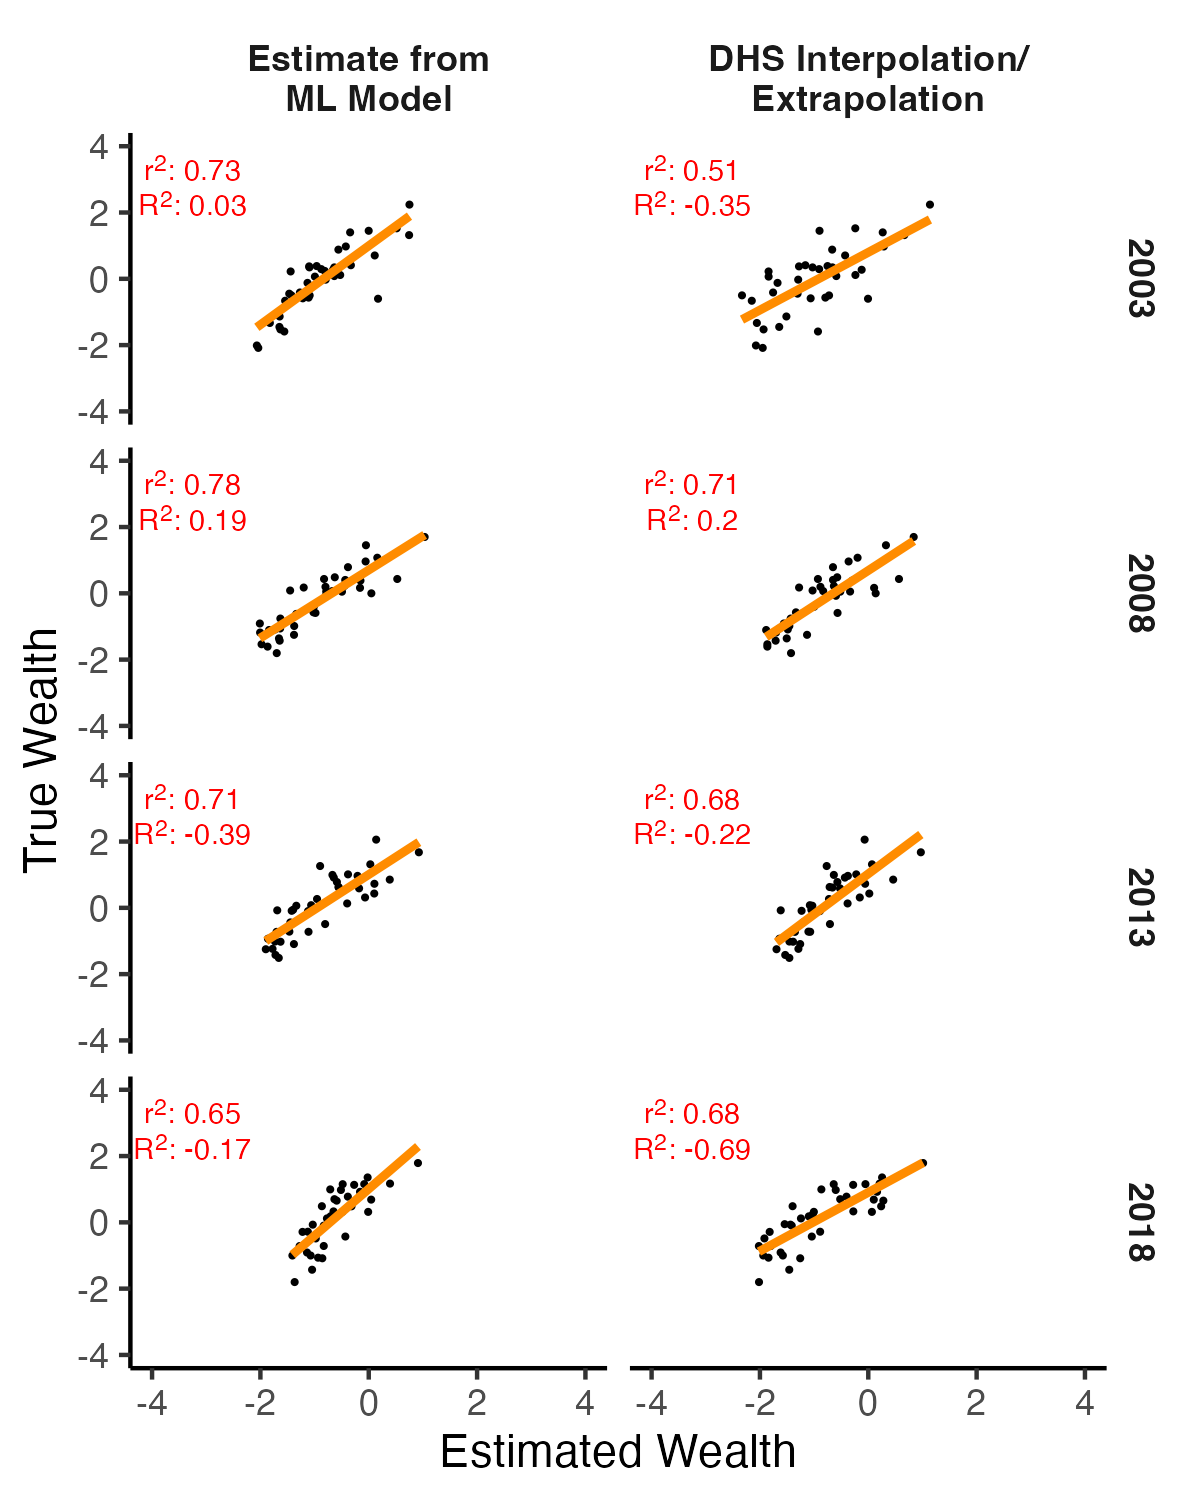
\includegraphics[width=0.9\textwidth]{figures/policy_exp_nigeria_gadm_1.png}
    \caption{Comparison of true wealth estimates versus estimates from machine learning model and using DHS data to interpolate and extrapolate wealth estimates; data is extrapolated for 2003 and 2018 data, and interpolated for 2008 and 2013. For each year, the two closest DHS rounds are used to estimate wealth; for example, the data in 2003 and 2013 is used to interpolate wealth for 2008. Wealth estimates are at the first administrative division level.}
     \label{fig:policy_exp_nigeria_gadm_1}
\end{figure}

% --------------------------
\newpage
\section{Comparing results across machine learning algorithms}
\label{si:ml_results_type}

\begin{figure}[H]
    \centering
    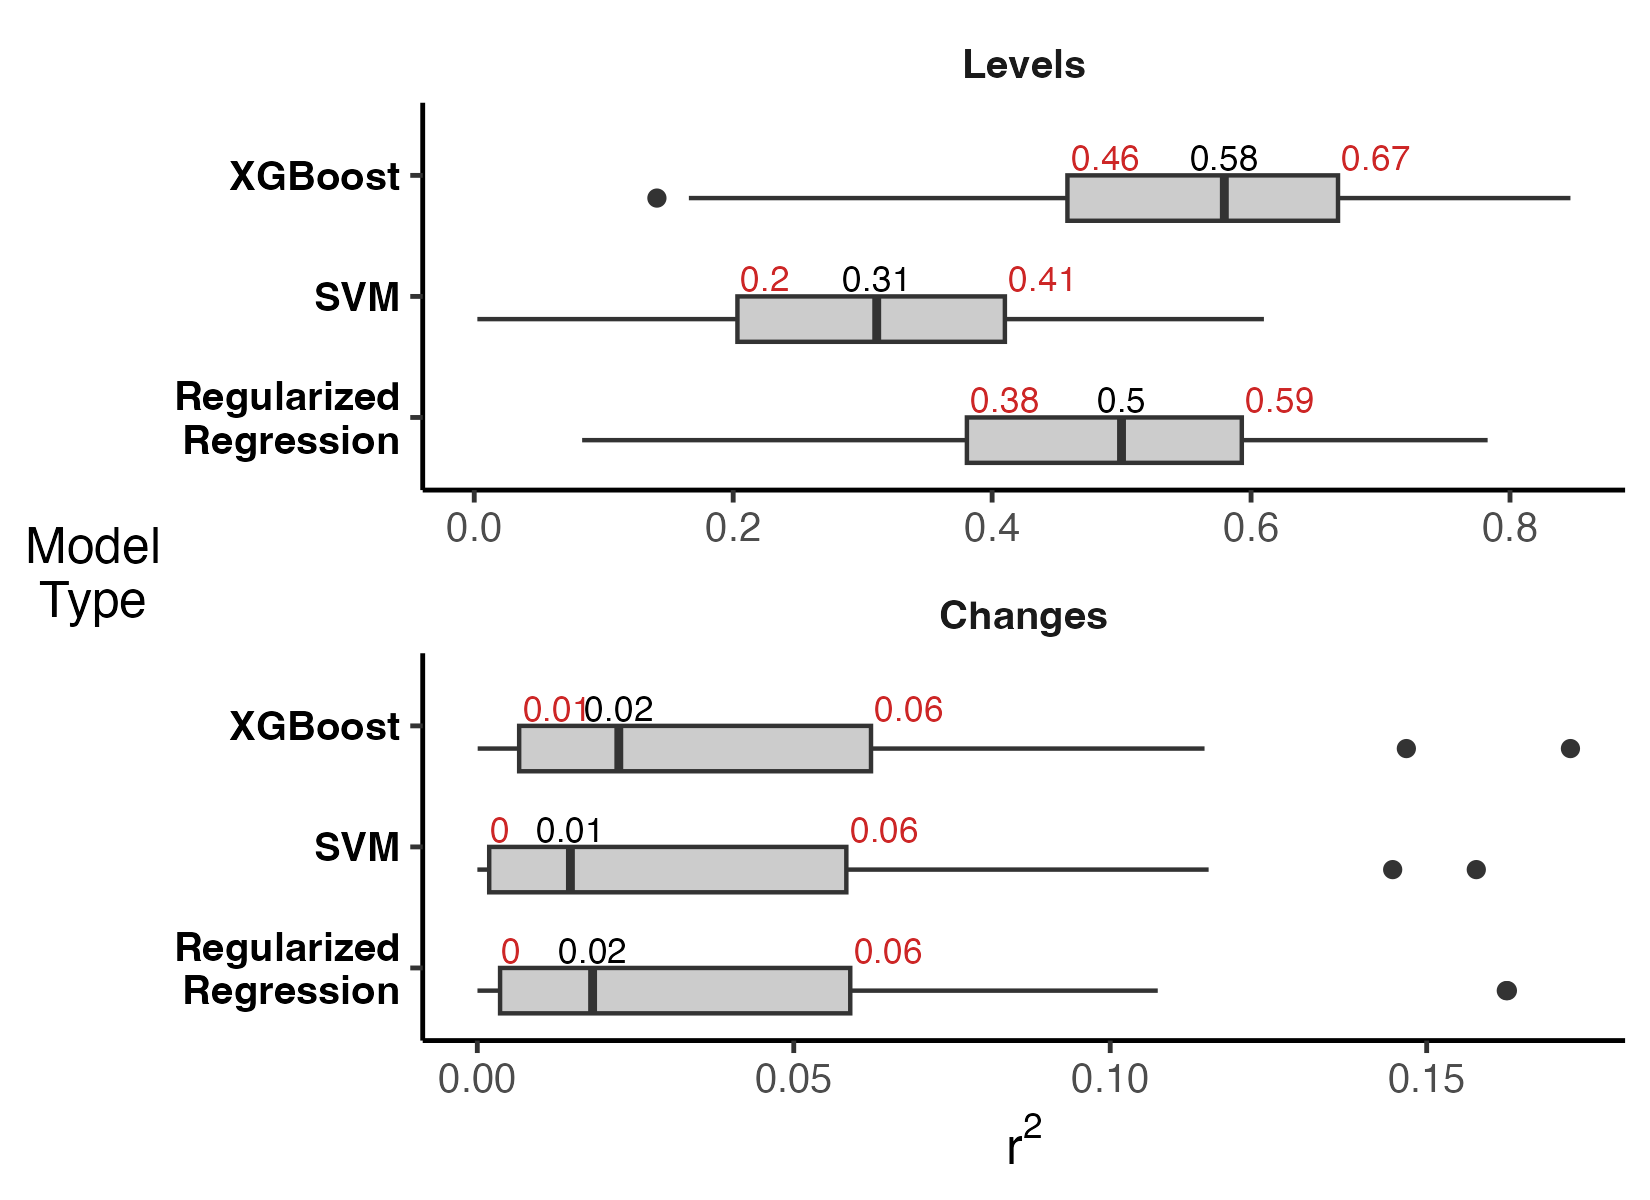
\includegraphics[width=0.9\textwidth]{figures/ml_results_type.png}
    \caption{Comparison of model performance by machine learning algorithm. The boxplots include: center line, median; box limits, upper and lower quartiles; whiskers, 1.5x interquartile range; points beyond whiskers, outliers.}
     \label{fig:ml_results_type}
\end{figure}

% --------------------------
\newpage
\section{Variation in wealth: within and across districts}\label{si:within_across_pca_sd}

\singlespacing
\begin{table}[H]
\small
\caption{Comparing standard deviation in wealth within and across districts}
\label{tab:within_across_pca_sd}
\centering
\begin{tabular}{lcc} 
\hline 
Country & Std. Dev. Wealth & Average Within District \\ 
         & Across Districts & Wealth Std. Dev. \\ 
 \hline 
Albania & 0.36 & 0.57 \\ 
 Angola & 1.19 & 0.86 \\ 
 Armenia & 0.22 & 0.42 \\ 
 Bangladesh & 0.64 & 0.74 \\ 
 Benin & 0.8 & 0.78 \\ 
 Bolivia & 0.99 & 1.14 \\ 
 Burkina Faso & 0.64 & 0.79 \\ 
 Burundi & 0.79 & 0.47 \\ 
 Cambodia & 0.93 & 0.62 \\ 
 Cameroon & 1.05 & 1 \\ 
 Chad & 0.55 & 0.65 \\ 
 Colombia & 1.12 & 0.91 \\ 
 Comoros & 0.99 & 0.98 \\ 
 Congo - Kinshasa & 0.88 & 0.35 \\ 
 Côte d’Ivoire & 0.73 & 1.31 \\ 
 Dominican Republic & 0.57 & 0.64 \\ 
 Egypt & 0.53 & 0.34 \\ 
 Eswatini & 1.09 & 0.88 \\ 
 Ethiopia & 0.92 & 0.79 \\ 
 Gabon & 0.78 & 1.04 \\ 
 Gambia & 1 & 0.75 \\ 
 Ghana & 0.94 & 0.63 \\ 
 Guatemala & 1.08 & 0.76 \\ 
 Guinea & 0.97 & 0.97 \\ 
 Guyana & 1.29 & 0.54 \\ 
 Haiti & 0.62 & 0.84 \\ 
 Honduras & 0.88 & 0.82 \\ 
 India & 1.04 & 0.84 \\ 
 Indonesia & 1.06 & 0.81 \\ 
 Jordan & 0.41 & 0.36 \\ 
 Kenya & 1 & 0.96 \\ 
 Kyrgyzstan & 0.61 & 0.47 \\ 
 Lesotho & 0.65 & 1.33 \\ 
 Liberia & 0.56 & 0.47 \\ 
 Madagascar & 0.49 & 1.05 \\ 
 Malawi & 0.99 & 0.76 \\ 
 Mali & 0.89 & 0.8 \\ 
 Moldova & 0.44 & 0.71 \\ 
 Morocco & 1.16 & 1.5 \\ 
 Mozambique & 1.41 & 1.01 \\ 
 Myanmar (Burma) & 0.83 & 0.84 \\ 
 Namibia & 1.77 & 1.15 \\ 
 Nepal & 0.7 & 0.98 \\ 
 Niger & 0.88 & 0.82 \\ 
 Nigeria & 1.16 & 0.71 \\ 
 Pakistan & 0.9 & 1.19 \\ 
 Peru & 1.16 & 1.21 \\ 
 Philippines & 0.77 & 0.52 \\ 
 Rwanda & 0.62 & 0.75 \\ 
 Senegal & 1.23 & 1.13 \\ 
 Sierra Leone & 0.75 & 0.8 \\ 
 South Africa & 1.05 & 1.13 \\ 
 Tajikistan & 0.7 & 0.61 \\ 
 Tanzania & 1 & 0.72 \\ 
 Timor-Leste & 0.87 & 0.91 \\ 
 Togo & 0.66 & 0.82 \\ 
 Uganda & 1 & 0.56 \\ 
 Zambia & 1.13 & 1.23 \\ 
 Zimbabwe & 1.29 & 1.24 \\ 
 \hline 
\end{tabular}
\end{table}
\normalsize
\doublespacing

% --------------------------
\newpage

\section{Comparison of results to other papers}
\label{si:compare_other_papers}


\singlespacing
\begin{table}[H]
\caption{Comparison of results to other papers. Yeh et al. (2020) and Chi et al. (2022) use models trained on other countries to estimate wealth in each country of interest; consequently, when comparing our results to these paper, we show results from models using a similar approach---where models are trained on all other countries. For each country, Jean et al. (2016) trains models using only data for each country; consequently, when comparing our results to this paper, we show results from models using a similar approach---where models are trained on data within each country.}
\label{fig:compare_other_papers}
\centering 
\begin{tabular}{lllllll}
\hline
Unit & Level/Change & Aggregation & Location & Paper & Other       & This \\
     &              &             &          &       & Paper $r^2$ & Paper $r^2$ \\

\hline
Village  & Levels  & Pooled                   & Africa         & Yeh et al. (2020) & 0.67 & 0.75 \\
Village  & Levels  & Average across countries & Africa         & Yeh et al. (2020) & 0.7 & 0.60 \\
Village  & Levels  & Pooled                   & Africa - Urban & Yeh et al. (2020) & 0.4 & 0.61 \\
Village  & Levels  & Pooled                   & Africa - Rural & Yeh et al. (2020) & 0.32 & 0.65 \\
District & Levels  & Pooled                   & Africa         & Yeh et al. (2020) & 0.75 & 0.78 \\
District & Levels  & Average across countries & Africa         & Yeh et al. (2020) & 0.83 & 0.66 \\
Village  & Changes & Pooled                   & Africa         & Yeh et al. (2020) & 0.35 & 0.04  \\
District & Changes & Pooled                   & Africa         & Yeh et al. (2020) & 0.43 & 0.05  \\
\hline
Village & Levels   & Average across countries & All DHS countries & Chi et al. (2022) & 0.59 & 0.55 \\
\hline 
Village & Levels   & Not applicable           & Malawi            & Jean et al. (2016) & 0.55 & 0.48 \\
Village & Levels   & Not applicable           & Nigeria           & Jean et al. (2016) & 0.68 & 0.70 \\
Village & Levels   & Not applicable           & Rwanda            & Jean et al. (2016) & 0.75 & 0.58 \\
Village & Levels   & Not applicable           & Tanzania          & Jean et al. (2016) & 0.57 & 0.69 \\
Village & Levels   & Not applicable           & Uganda            & Jean et al. (2016) & 0.69 & 0.76 \\
\hline 
\end{tabular}
\end{table}
\doublespacing

% --------------------------
\newpage
\section{Wealth asset index and consumption comparison}
\label{si:asset_vs_consumption}

\begin{figure}[H]
    \centering
    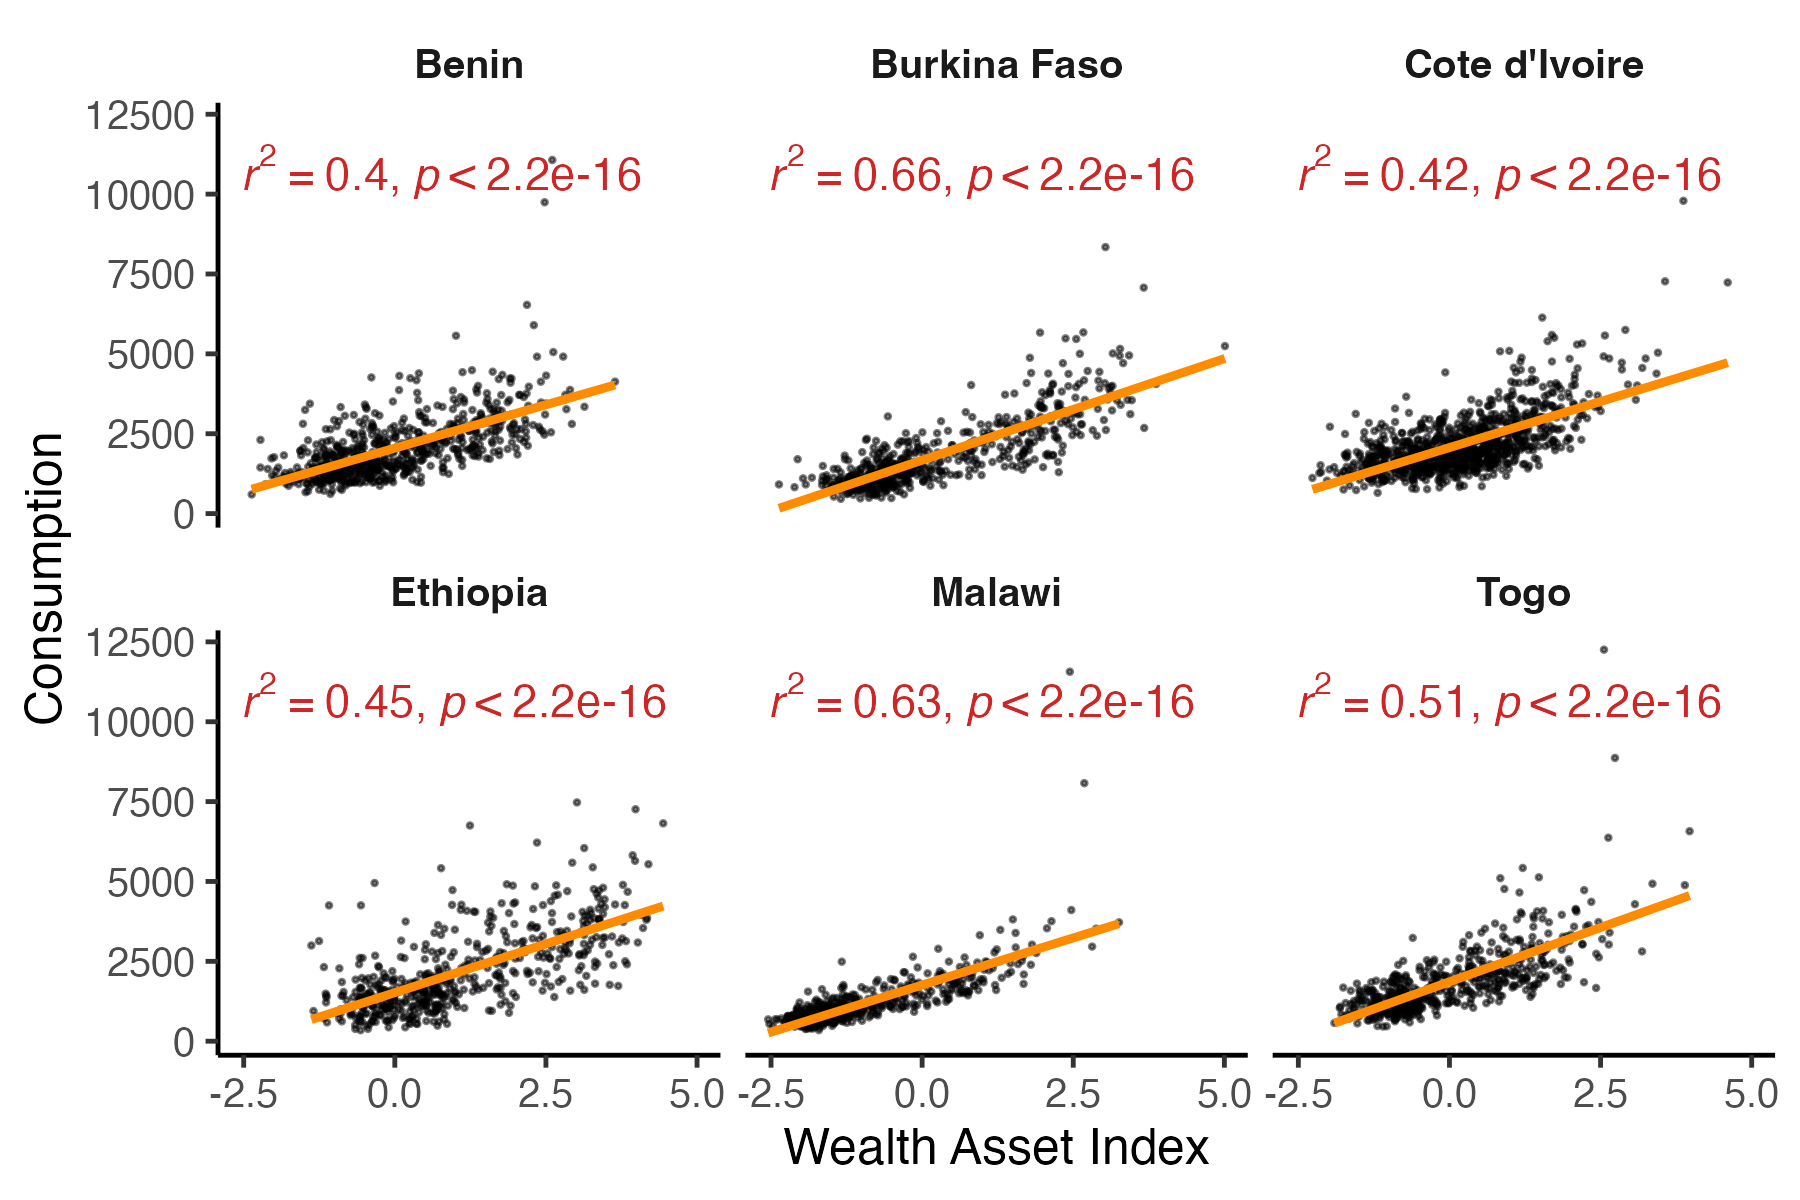
\includegraphics[width=0.9\textwidth]{figures/lsms_pov_measure_cor.png}
    \caption{Comparison of wealth asset index and consumption}
     \label{fig:lsms_pov_measure_cor}
\end{figure}

\begin{figure}[H]
    \centering
    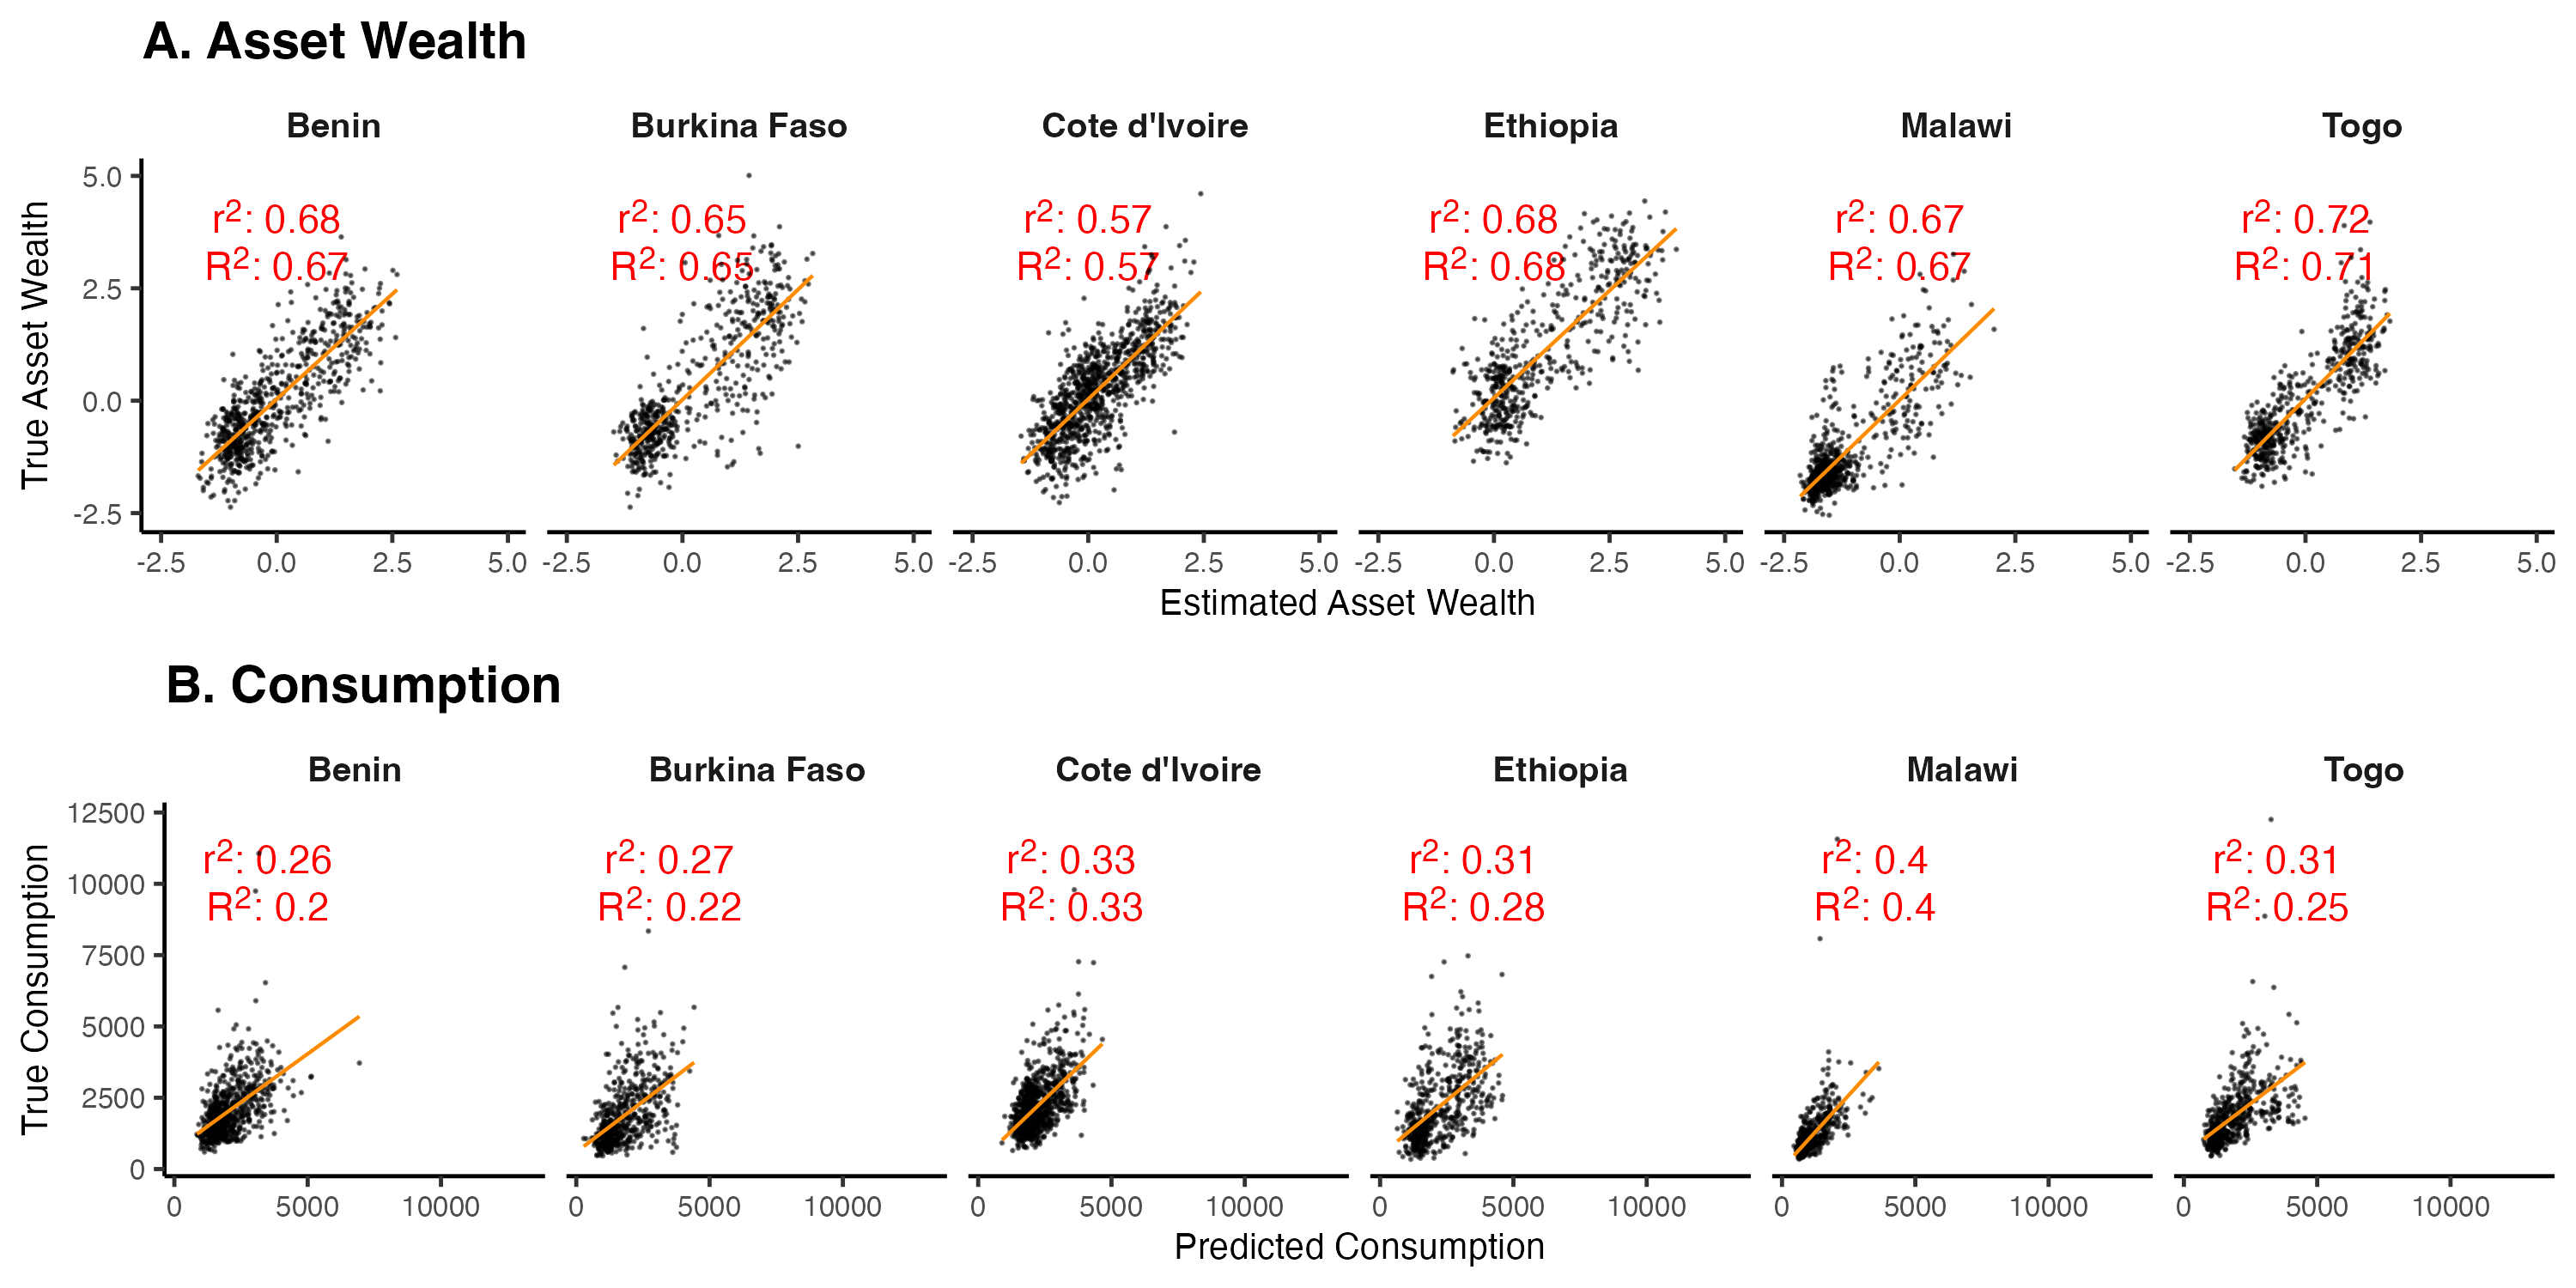
\includegraphics[width=0.9\textwidth]{figures/lsms_r2.png}
    \caption{Comparison of model performance estimating wealth asset index and consumption}
     \label{fig:lsms_r2}
\end{figure}

\begin{figure}[H]
    \centering
    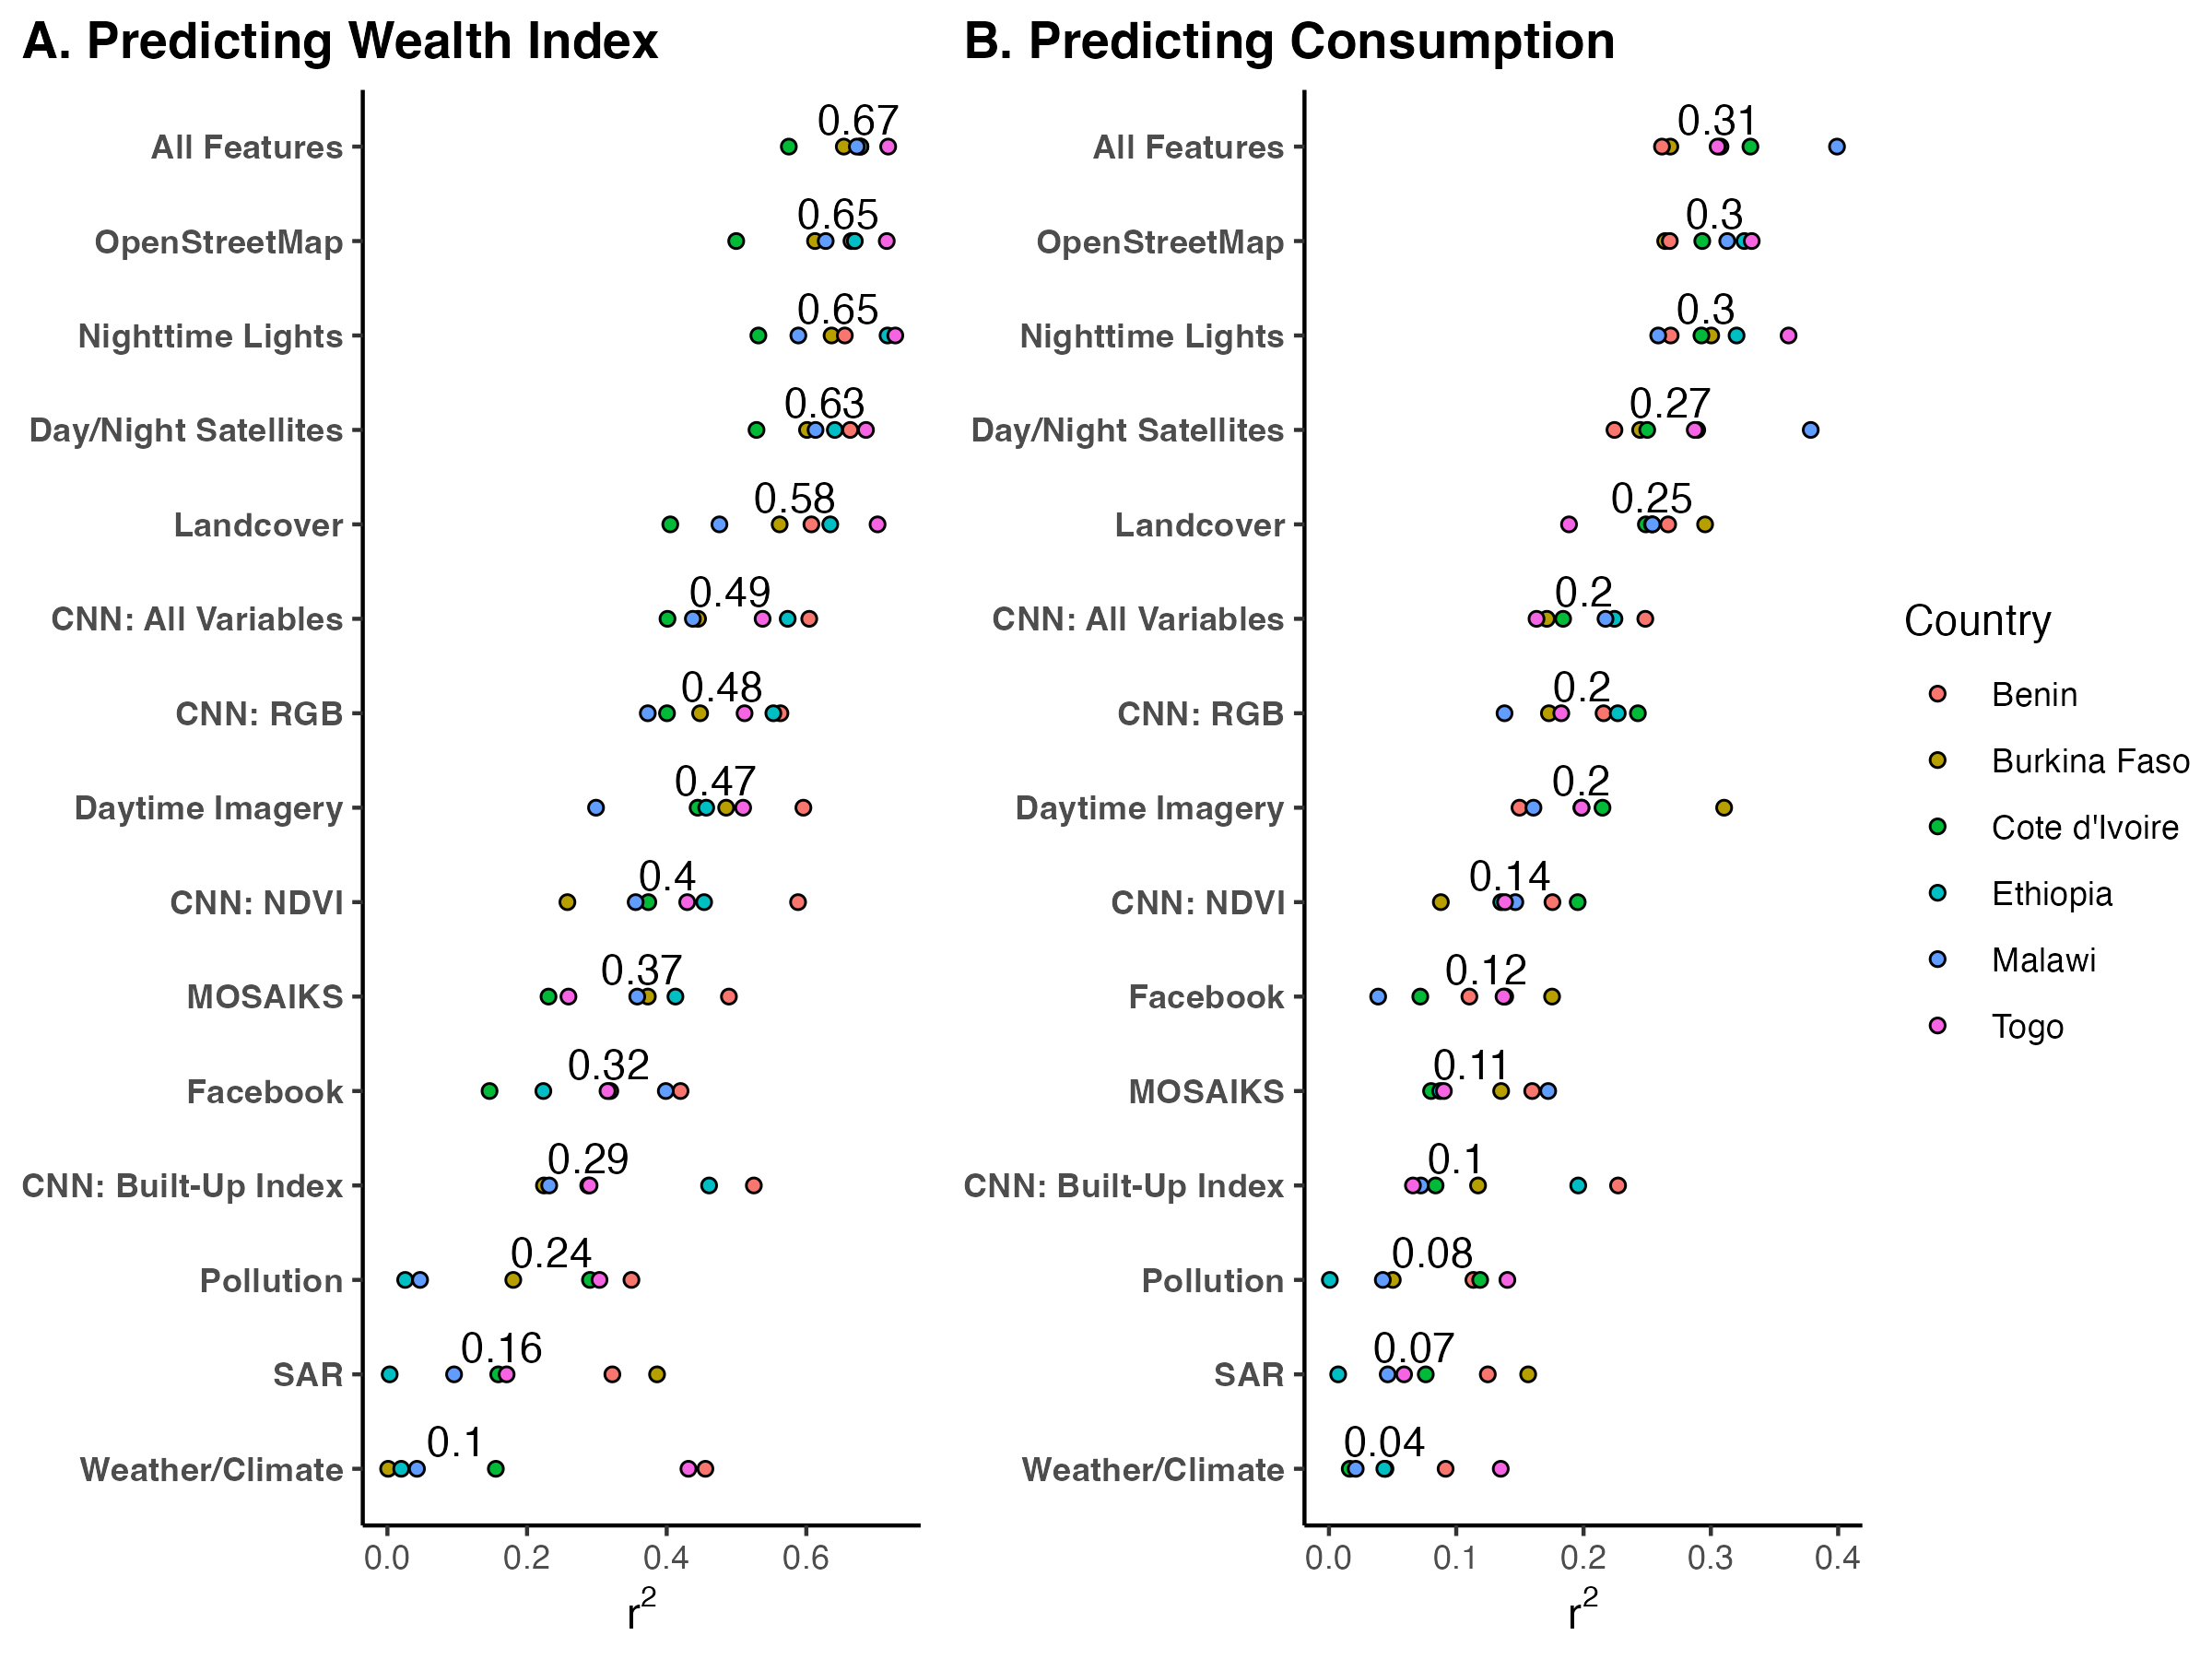
\includegraphics[width=0.9\textwidth]{figures/lsms_feature_type.png}
    \caption{Comparison of model performance estimating wealth asset index and consumption by set of features used to train the model. The median $r^2$ is reported.}
     \label{fig:lsms_feature_type}
\end{figure}

\color{black}

% --------------------------
\newpage
\section{Comparing DHS and Facebook education variables}
\label{si:wi_and_fb_edu}

\begin{figure}[H]
    \centering
    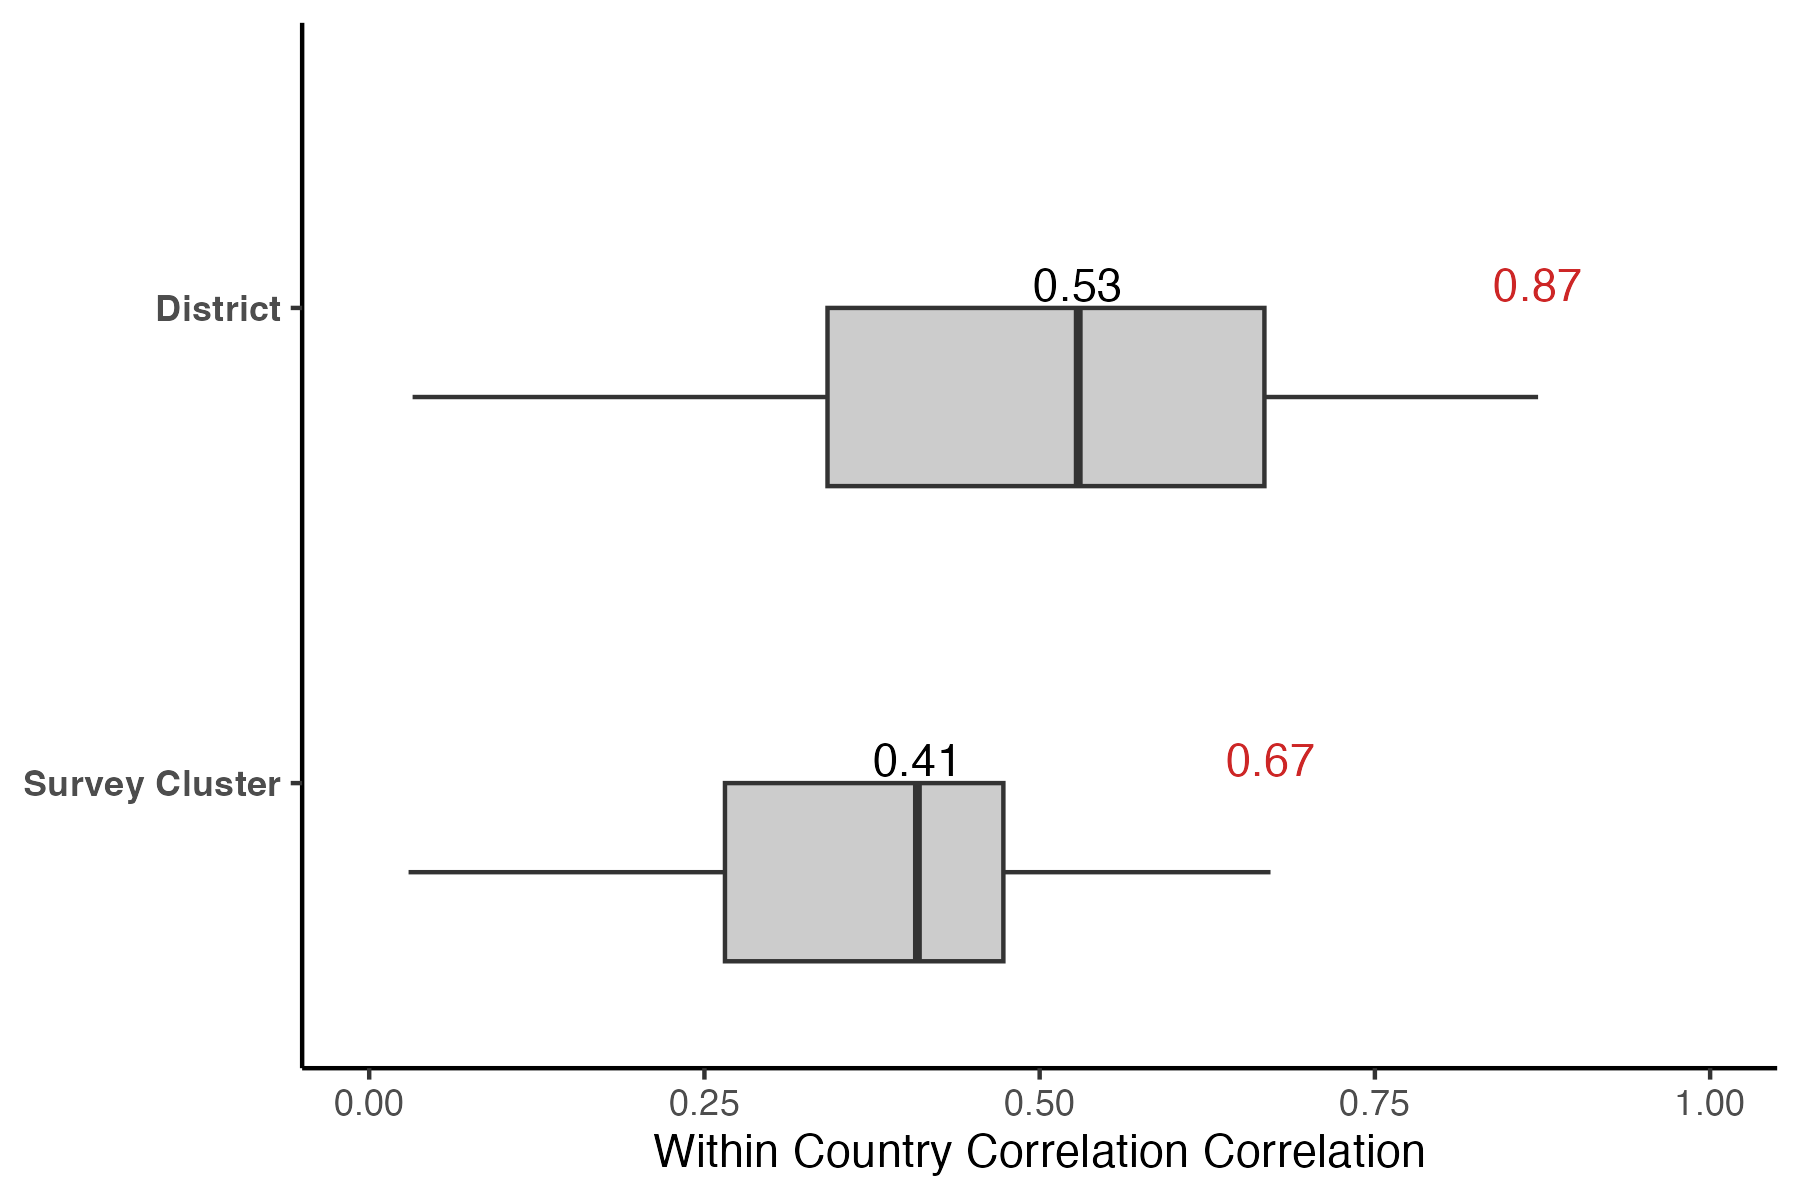
\includegraphics[width=0.5\textwidth]{figures/educ_fb_dhs_boxplot.png}
    \caption{Distribution of within-country correlation between the proportion of the population with above high school education as measured by DHS and Facebook. The boxplots include: center line, median; box limits, upper and lower quartiles; whiskers, 1.5x interquartile range; points beyond whiskers, outliers.}
     \label{fig:educ_fb_dhs_boxplot}
\end{figure}

\begin{figure}[H]
    \centering
    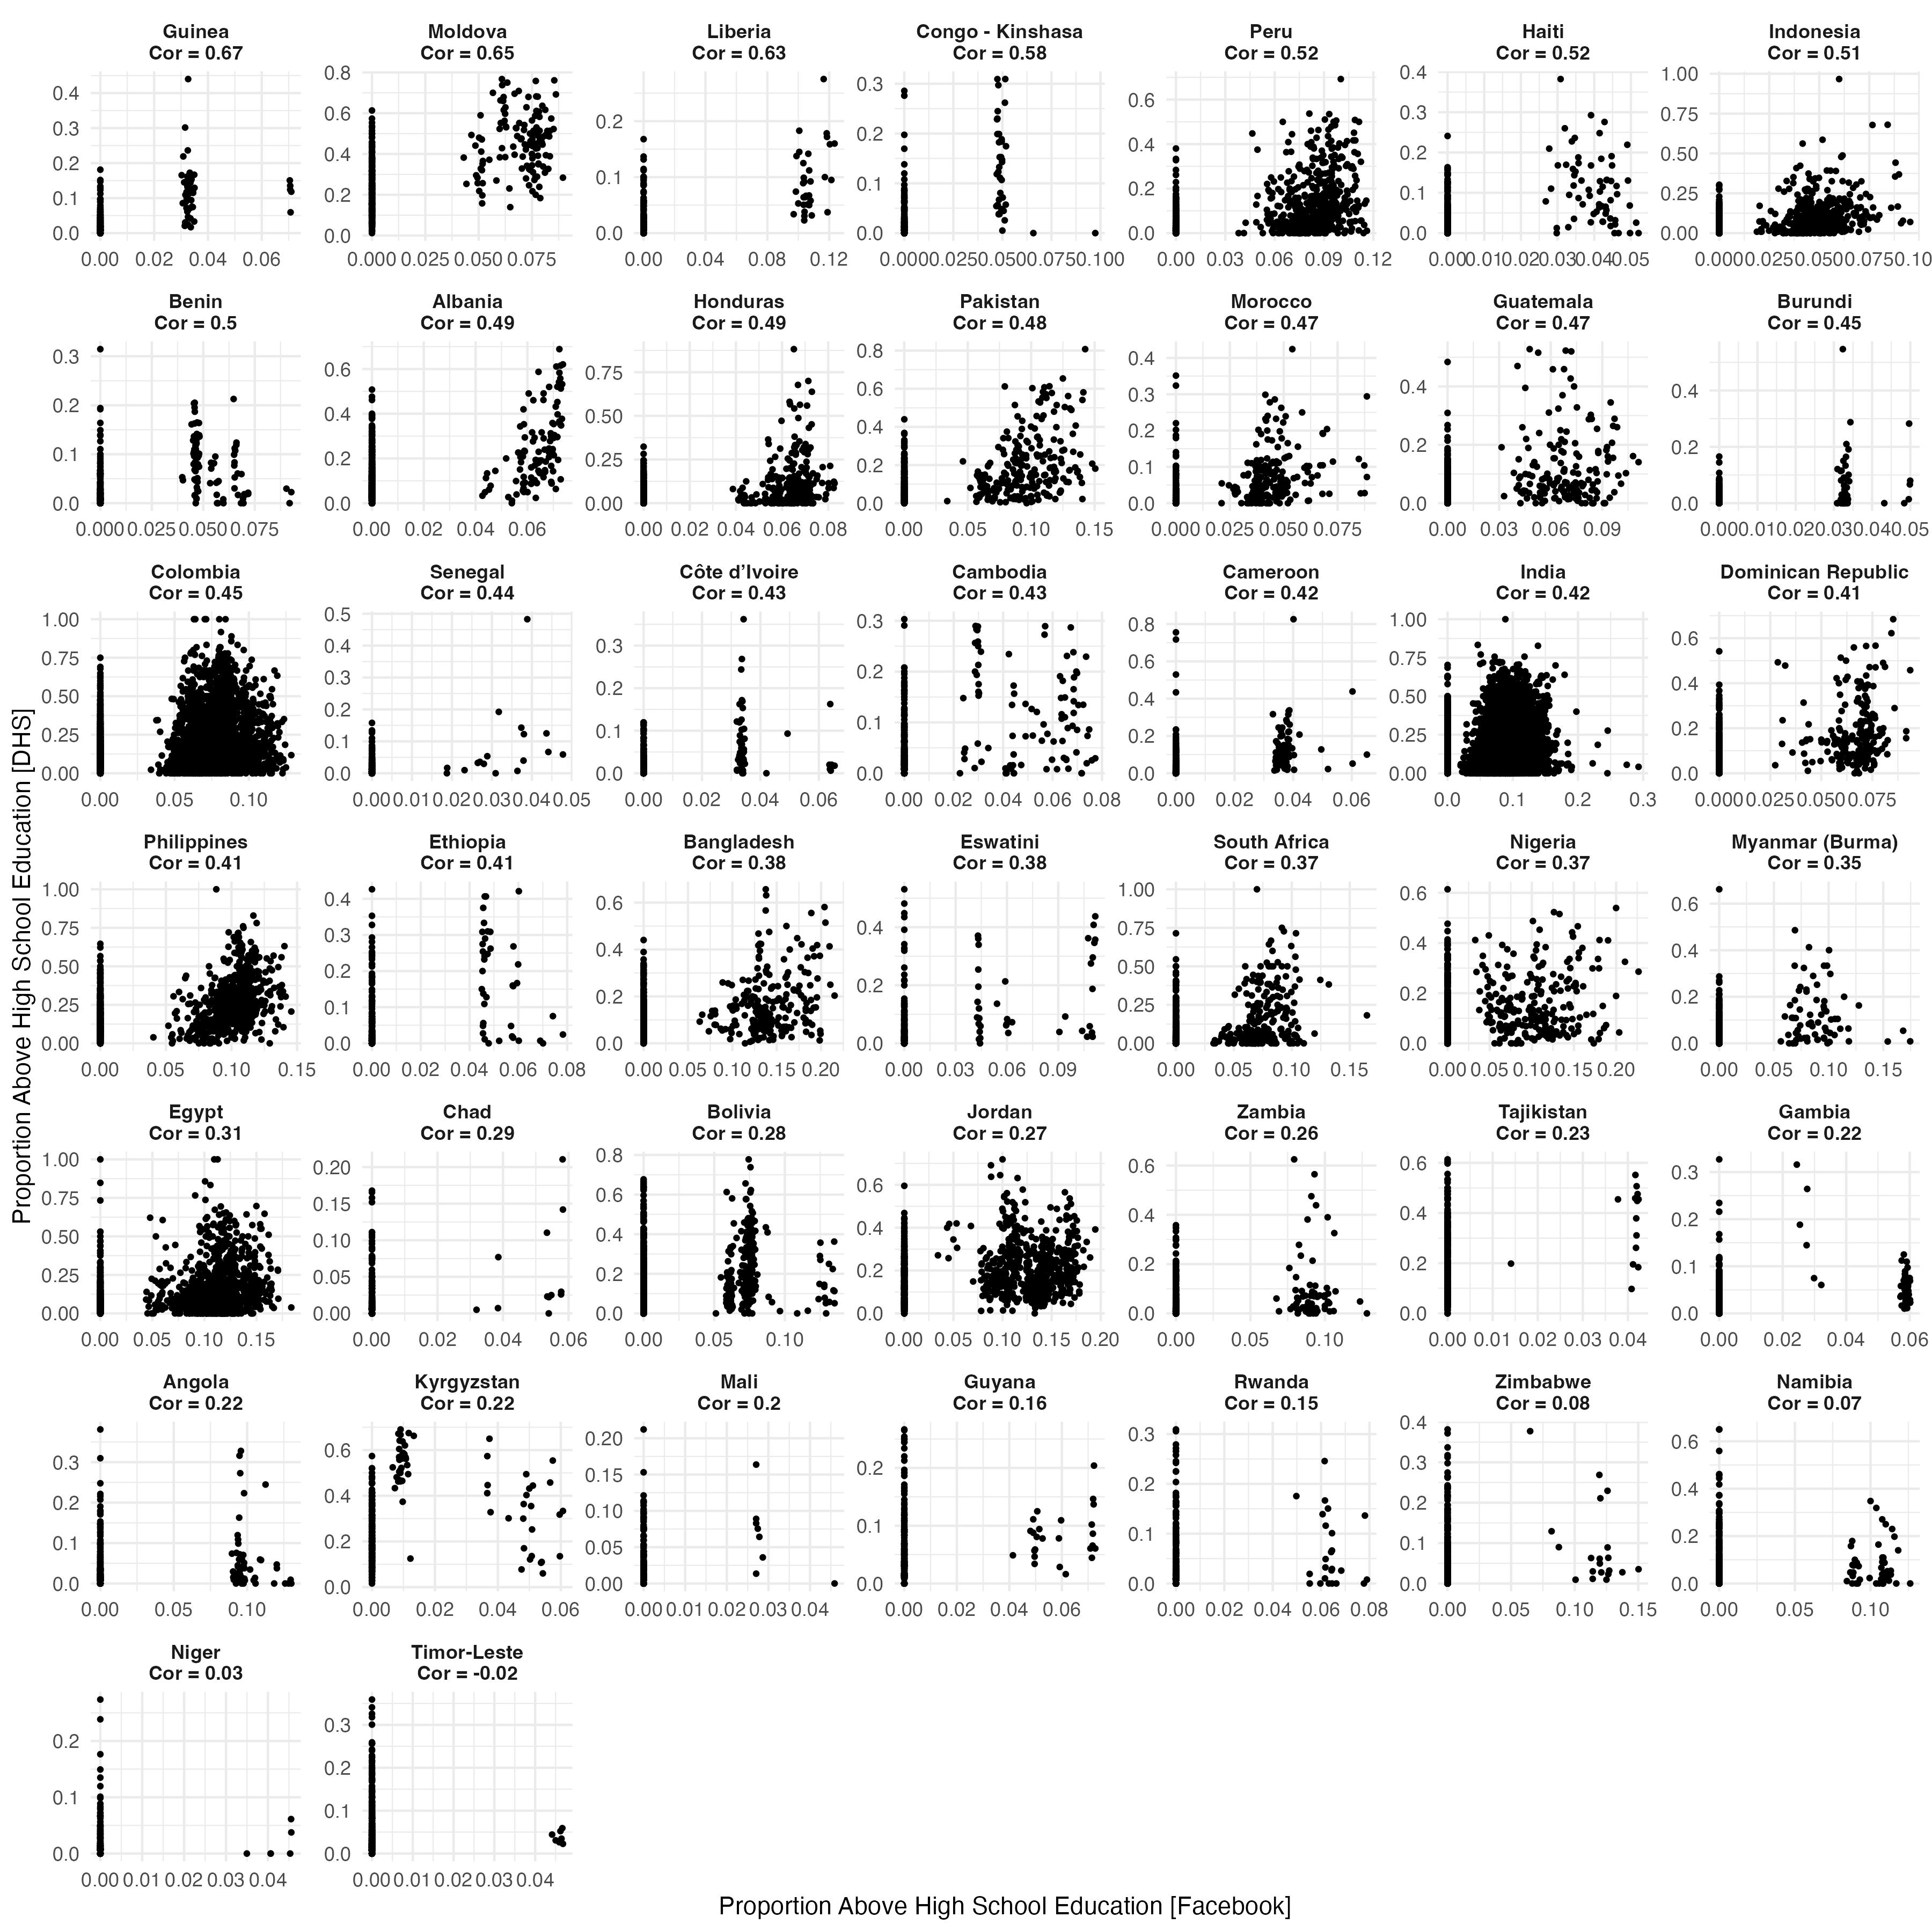
\includegraphics[width=1\textwidth]{figures/educ_fb_dhs_scatter_cluster.png}
    \caption{Cluster-level scatterplot between proportion with above high school education as measured by Facebook and DHS}
     \label{fig:educ_fb_dhs_scatter_cluster}
\end{figure}

\begin{figure}[H]
    \centering
    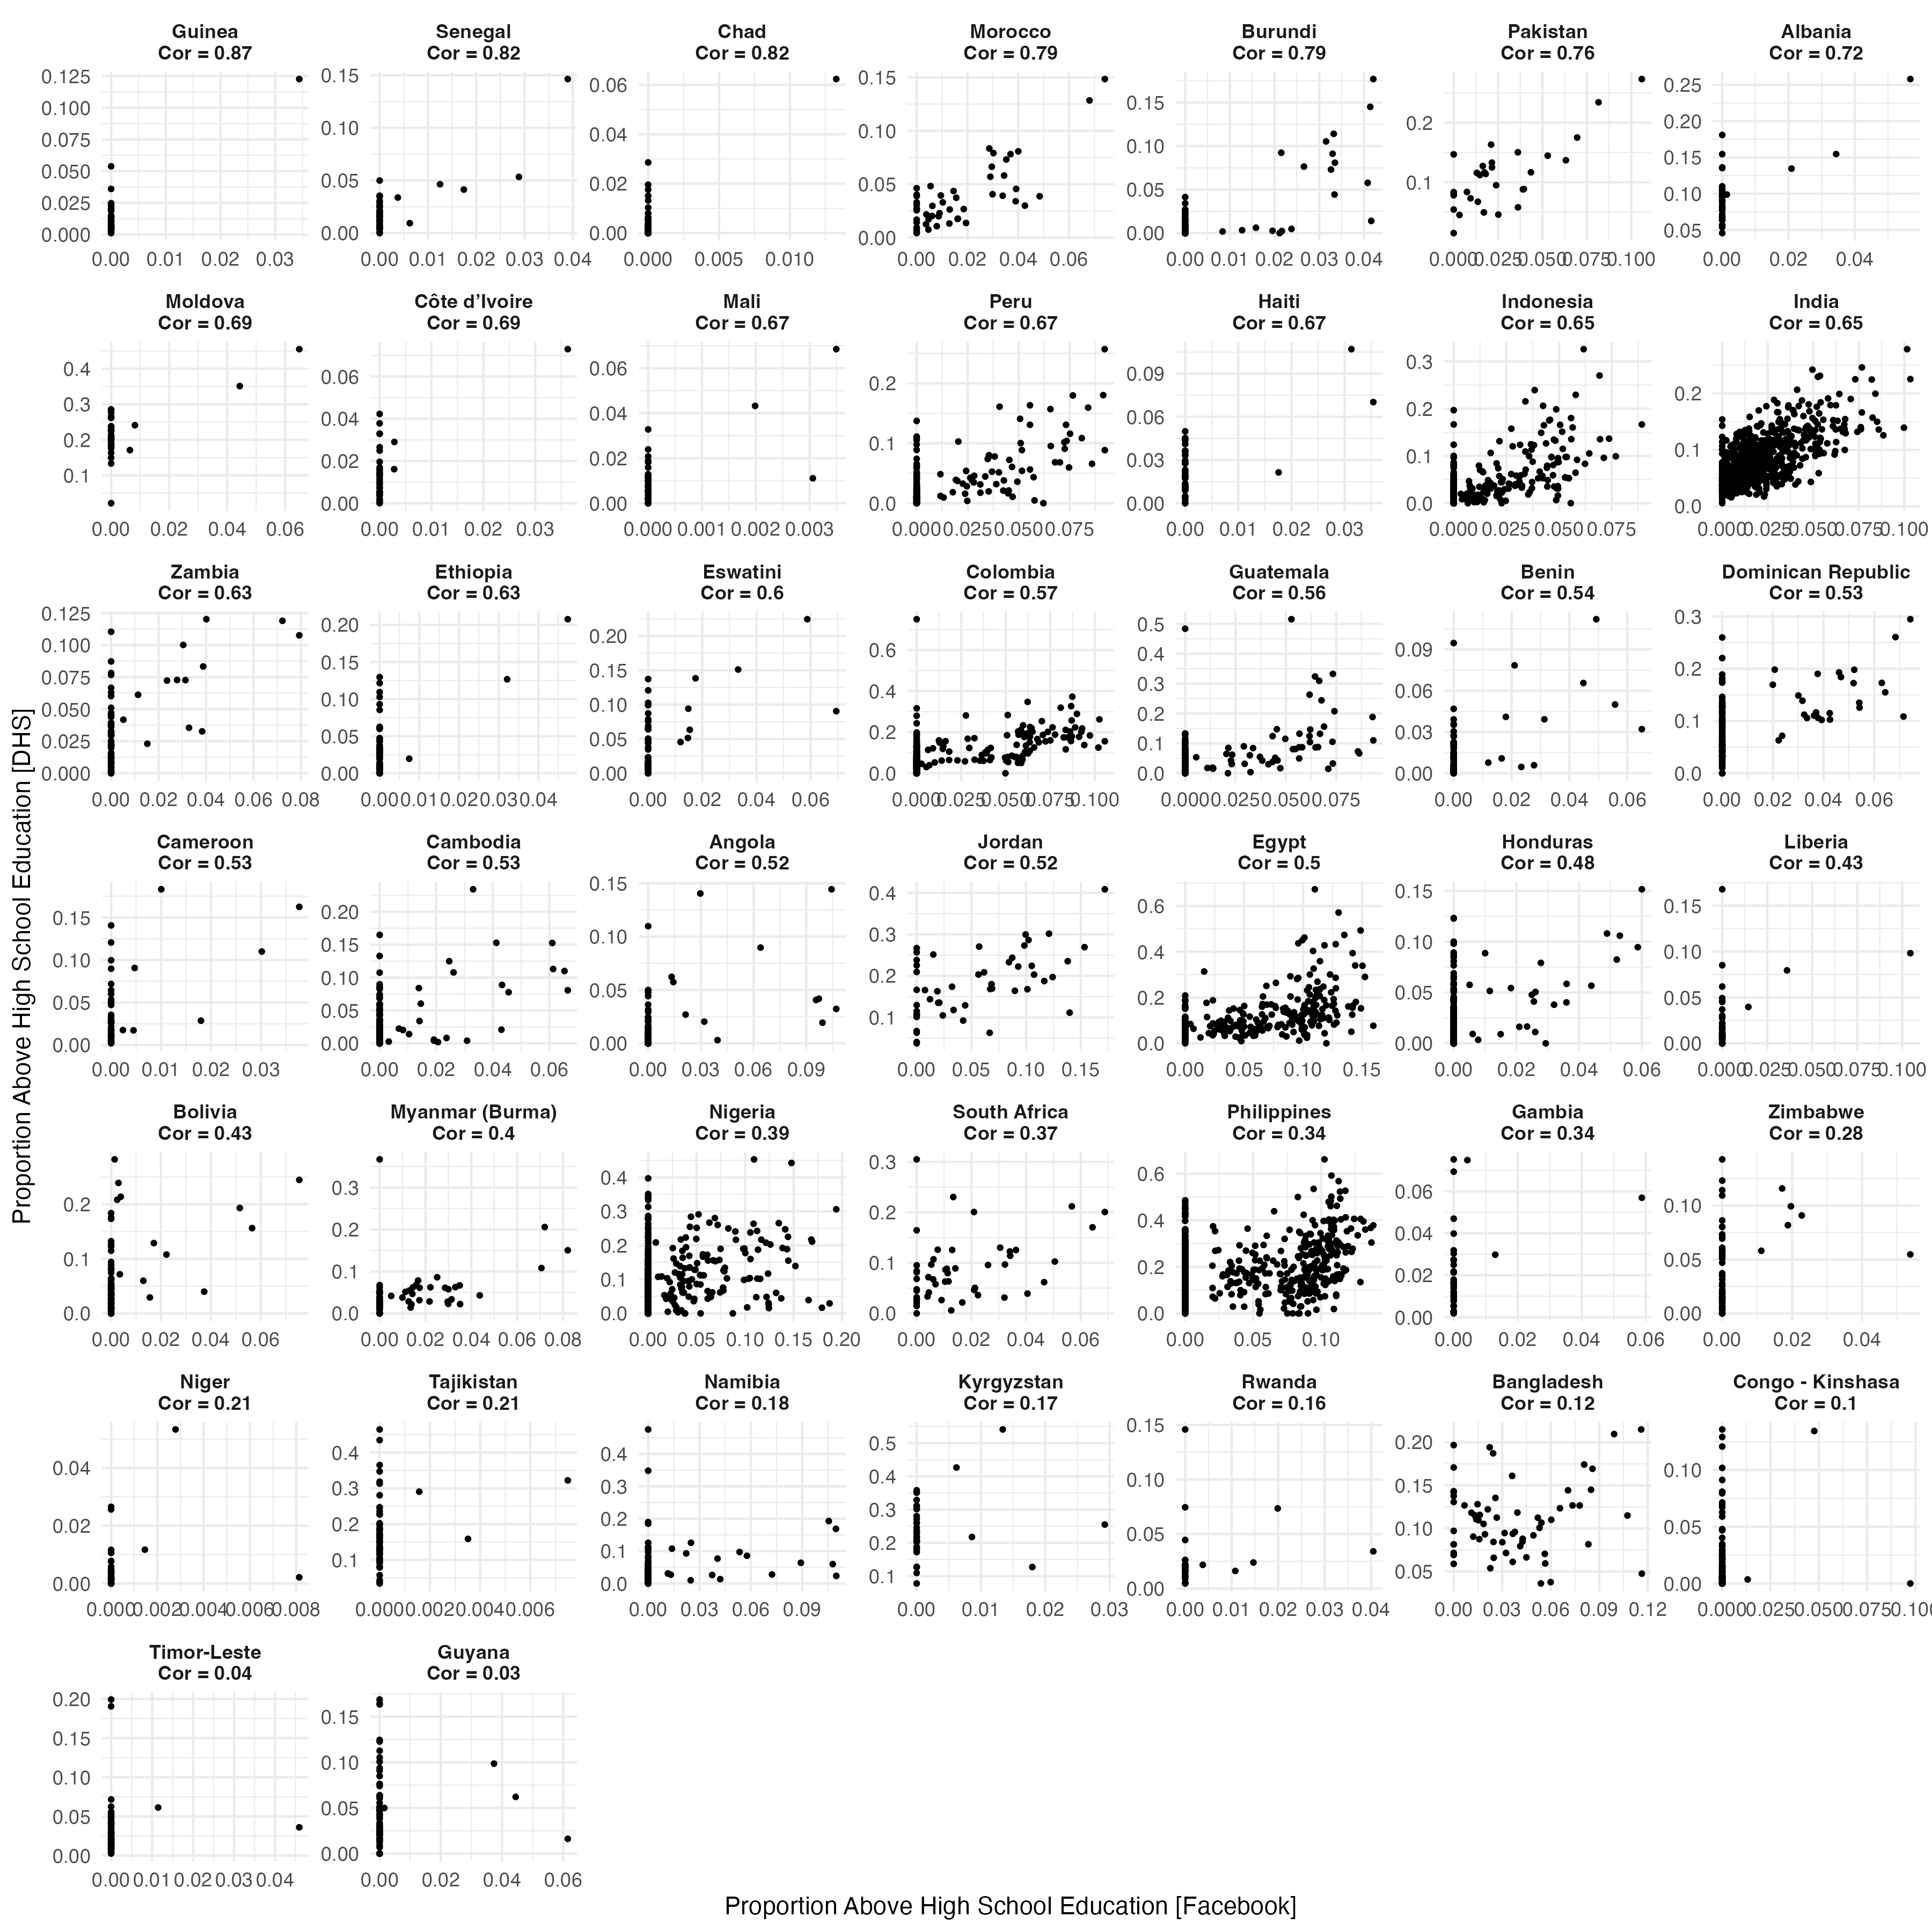
\includegraphics[width=1\textwidth]{figures/educ_fb_dhs_scatter_adm2.png}
    \caption{District-level scatterplot between proportion with above high school education as measured by Facebook and DHS}
     \label{fig:educ_fb_dhs_scatter_adm2}
\end{figure}

\begin{figure}[H]
    \centering
    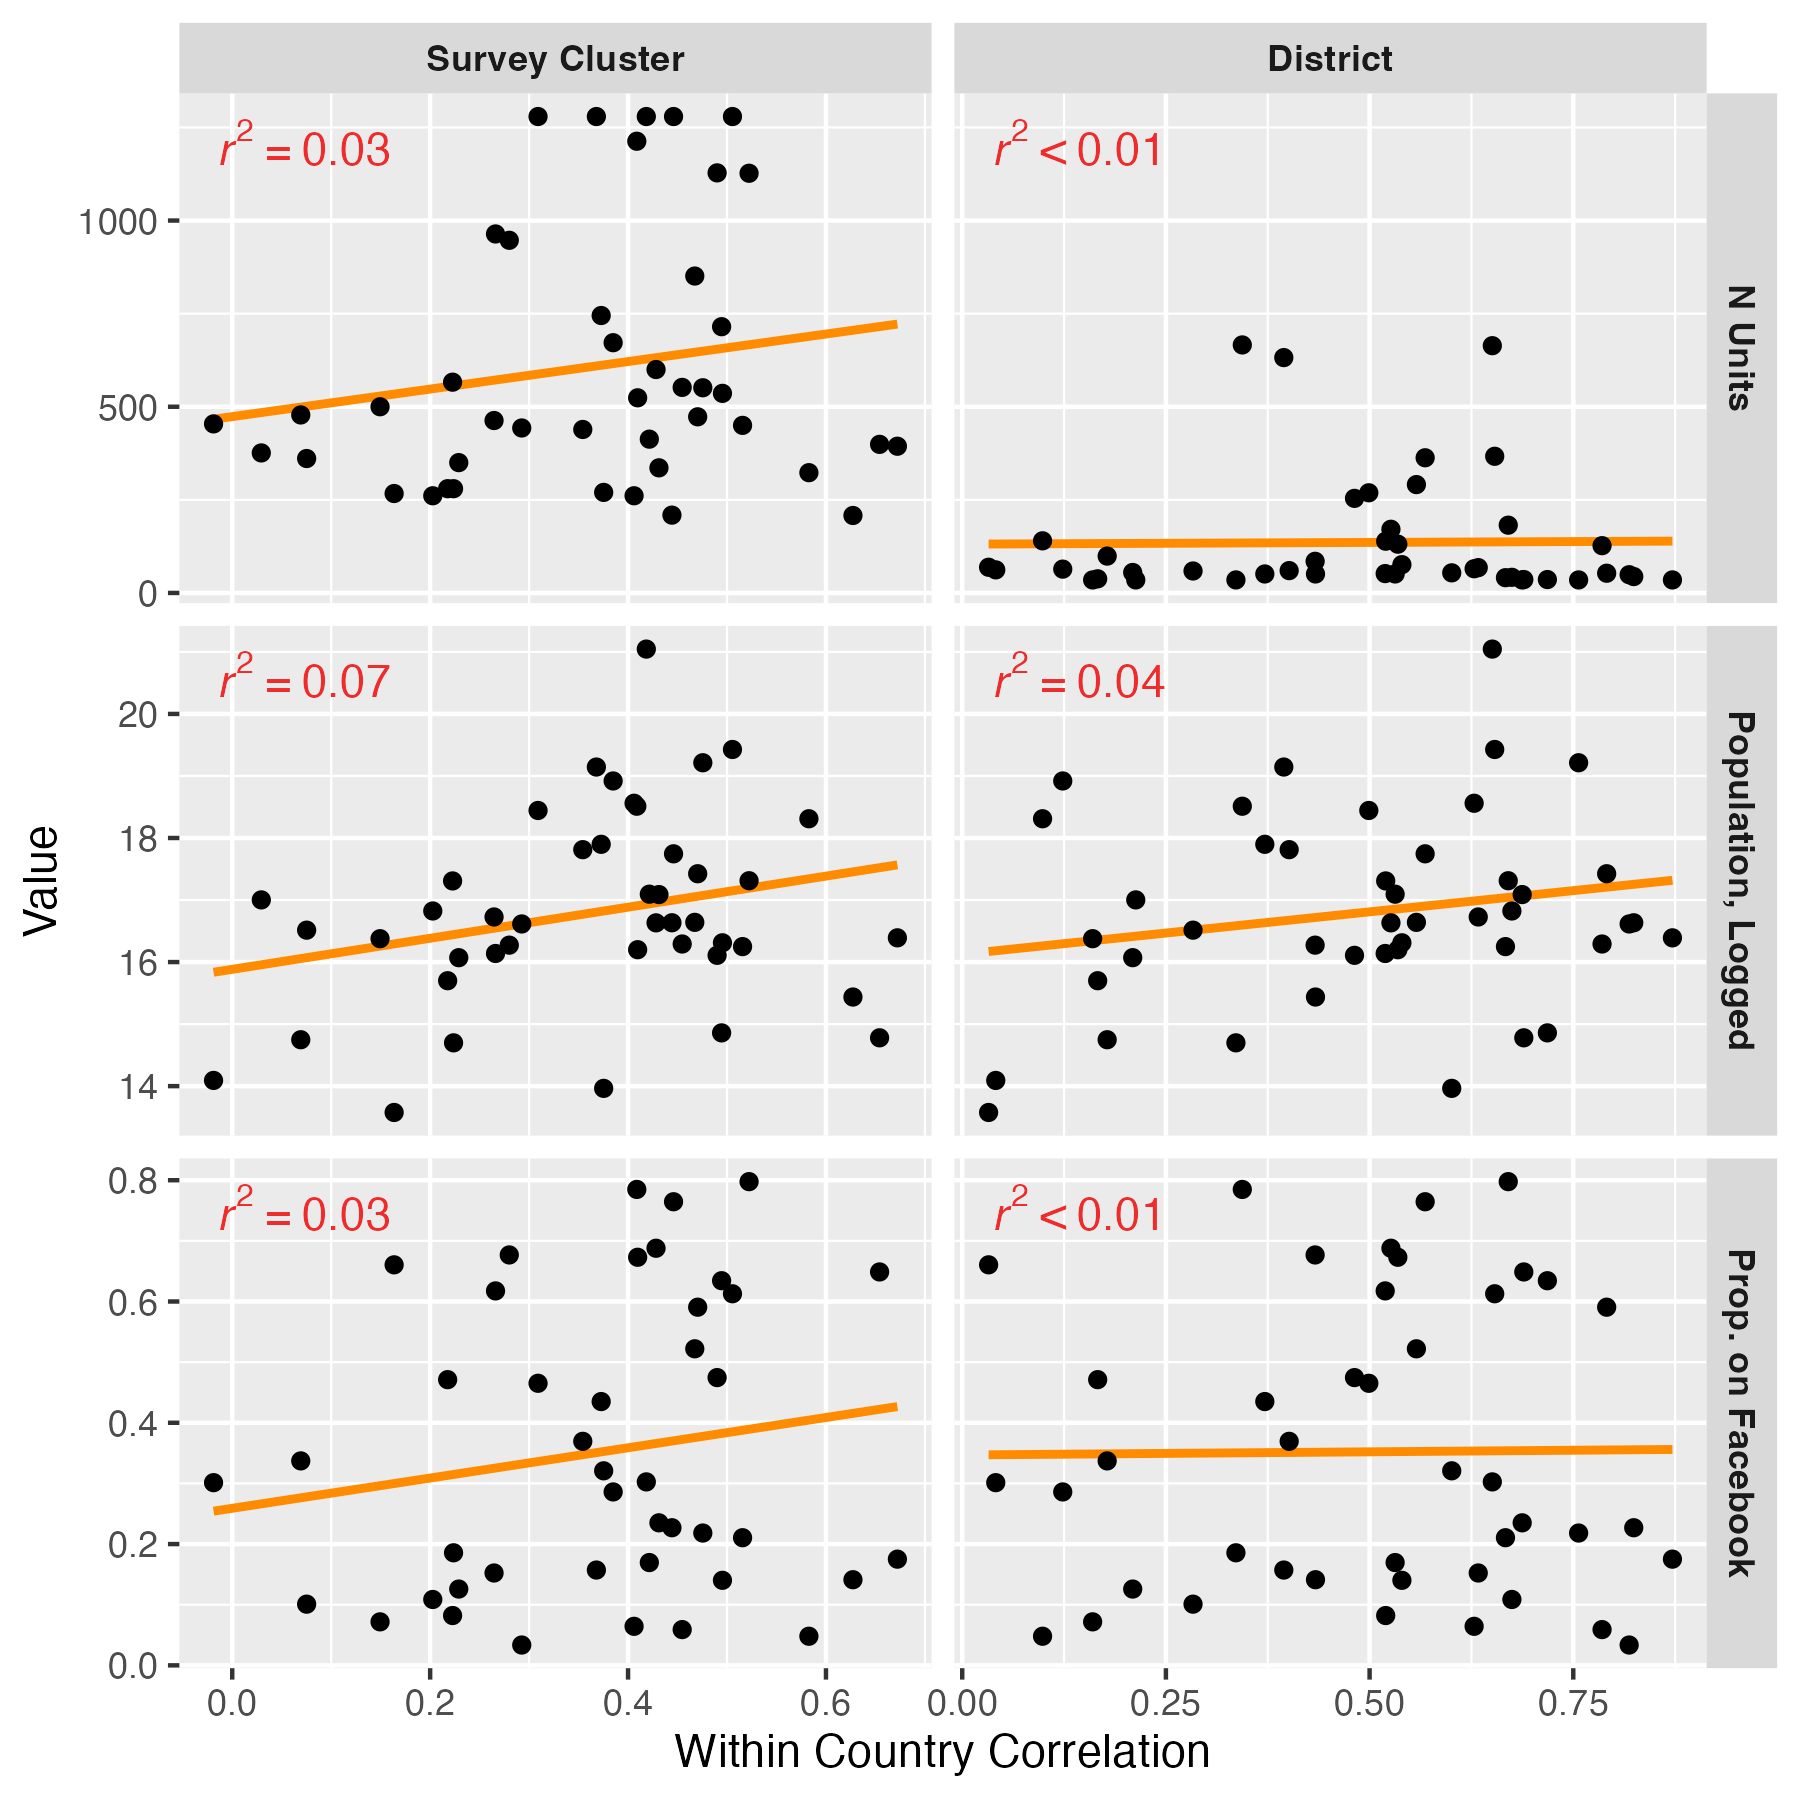
\includegraphics[width=0.8\textwidth]{figures/educ_fb_dhs_explain.png}
    \caption{Scatterplot between (1) within country correlation of the proportion with above high school education as measured by Facebook and DHS, and (2) country-level features}
     \label{fig:educ_fb_dhs_explain}
\end{figure}


\end{document}